%!Mode:: "TeX:System

%%%%%%%%%%%%%%%%%%%%%%%%%%%%%%%%%%%%%%%%%%%%%%%%%%%%%%%%%%%%%%%%%%%%%%%%%%%%%
%                                                                           %
%          LaTeX File for Doctor (Master) Thesis of ECNU                    %
%            华东师范大学博士(硕士)论文模板 ____lizb                      %
%                                                                           %
%%%%%%%%%%%%%%%%%%%%%%%%%%%%%%%%%%%%%%%%%%%%%%%%%%%%%%%%%%%%%%%%%%%%%%%%%%%%%




\documentclass[12pt,openany,a4paper,fancyhdr,twoside]{ctexbook}

%draft 选项可以使插入的图形只显示外框,以加快预览速度。
%\documentclass[11pt,a4paper,openany,draft]{book}
\usepackage{amsmath}
\usepackage{amssymb}               % AMSLaTeX宏包 用来排出更加漂亮的公式
%\usepackage[CJKbookmarks]{hyperref}
\usepackage{url}
\usepackage[hidelinks]{hyperref}
\usepackage{shortvrb,indentfirst,ulem,makeidx}
\usepackage{fancyhdr}
\usepackage{graphicx}

\usepackage{rotating}


\usepackage{indentfirst,latexsym,colortbl,subfigure,clrscode}

%\usepackage[ruled,vlined,linesnumbered,]{algorithm2e}

\usepackage[linesnumbered,ruled,vlined,resetcount,algochapter]{algorithm2e}%[ruled,vlined]{
\usepackage{algorithmicx}
\usepackage{listings}
\usepackage{algcompatible}
\usepackage{algpseudocode}


\renewcommand*{\algorithmcfname}{算法}

\newcommand{\clearPaperPage}{\clearpage}
%$\renewcommand{\clearPaperPage}{\cleardoublepage}




\SetKwInput{KwIn}{\textbf{输入}}
\SetKwInput{KwOut}{\textbf{输出}}
\SetKwInput{KwReturn}{\textbf{return}}


\usepackage{bibspacing}

\setlength{\bibitemsep}{2\baselineskip plus .05\baselineskip minus .05\baselineskip}


\usepackage{bm}                     % 处理数学公式中的黑斜体的宏包
\usepackage{amssymb}                % AMSLaTeX宏包 用来排出更加漂亮的公式
\usepackage{mathrsfs}
\usepackage[subnum]{cases}
%\usepackage[numbers,sort&compress]{natbib}
\usepackage[super,square,comma,sort&compress]{natbib}
\usepackage{hypernat}
\usepackage{geometry}
\usepackage{times}
\usepackage{fontspec}
%\usepackage{libertine}
\usepackage{libertineotf}
\usepackage{caption}
\usepackage{titletoc}
\usepackage{mathtools}

%\usepackage{chngcntr}
\counterwithout{footnote}{chapter}



%\usepackage{cite}
\usepackage{longtable,booktabs}
\usepackage{multirow}
\usepackage{subfigure}
\usepackage[subfigure]{tocloft}

\usepackage{float}
\usepackage{balance}
\usepackage {paralist}
\usepackage{bbding}
\usepackage{pgffor}

\usepackage{threeparttable}


%\usepackage{biblatex}
\makeindex
\pagestyle{fancy}

\newcommand{\eat}[1]{}

\renewcommand{\headrulewidth}{0.4pt}
\fancyfoot[CO,CE]{\thepage}

\renewcommand{\algorithmicrequire}{\textbf{Input:}}
\renewcommand{\algorithmicensure}{\textbf{Output:}}

\newtheorem{Def}{定义}


\newcommand{\yihao}{\fontsize{26pt}{36pt}\selectfont}           % 一号, 1.4 倍行距
\newcommand{\erhao}{\fontsize{22pt}{28pt}\selectfont}          % 二号, 1.25 倍行距
\newcommand{\xiaoer}{\fontsize{18pt}{18pt}\selectfont}          % 小二, 单倍行距
\newcommand{\sanhao}{\fontsize{16pt}{24pt}\selectfont}        % 三号, 1.5 倍行距
\newcommand{\xiaosan}{\fontsize{15pt}{22pt}\selectfont}        % 小三, 1.5 倍行距
\newcommand{\sihao}{\fontsize{14pt}{21pt}\selectfont}            % 四号, 1.5 倍行距
\newcommand{\banxiaosi}{\fontsize{13pt}{19.5pt}\selectfont}    % 半小四, 1.5 倍行距
\newcommand{\xiaosi}{\fontsize{12pt}{18pt}\selectfont}            % 小四, 1.5 倍行距
\newcommand{\dawuhao}{\fontsize{11pt}{11pt}\selectfont}       % 大五号, 单倍行距
\newcommand{\wuhao}{\fontsize{10.5pt}{15.75pt}\selectfont}    % 五号, 单倍行距

\newcommand{\tablewuhao}{\fontsize{10.5pt}{12.5pt}\selectfont}    % 五号, 单倍行距

\newcommand{\equwuhao}{\fontsize{11.5pt}{15pt}\selectfont}

\renewcommand*{\bibfont}{\normalfont\normalsize\linespread{1}\selectfont}
\setlength{\bibitemsep}{\baselineskip}



%============================ 可以自定义文字块 ================================%


%交叉引用格式
\renewcommand\figureautorefname{图}
\renewcommand\tableautorefname{表}
\renewcommand\equationautorefname{式子}
\renewcommand{\algorithmautorefname}{算法}





\renewcommand{\contentsname}{\hfill\bfseries\Large 目录\hfill}
\renewcommand{\cftaftertoctitle}{\hfill}

\renewcommand{\listtablename}{\hfill\bfseries\Large 表~~~~格\hfill}
\renewcommand{\listfigurename}{\hfill\bfseries\Large 插~~~~图\hfill}


\renewcommand{\listalgorithmcfname}{\centering\bfseries\Large 算~~~~法}
\newcommand*{\fullref}[1]{\textbf{\hyperref[{#1}]{第\ref*{#1}章~}}}


%=============================段前段后定义=============================%
\def  \cftbeforetitleskip {35pt}
\def \cftaftertitleskip {25pt}
%% 目录部分
\setlength{\cftbeforetoctitleskip}{\cftbeforetitleskip}
\setlength{\cftaftertoctitleskip}{\cftaftertitleskip}

%% 图目录

\setlength{\cftbeforeloftitleskip}{\cftbeforetitleskip}
\setlength{\cftafterloftitleskip}{\cftaftertitleskip}

%% 表目录
\setlength{\cftbeforelottitleskip}{\cftbeforetitleskip}
\setlength{\cftafterlottitleskip}{\cftaftertitleskip}
%% 算法目录
%\setlength{\cftbeforeloatitleskip}{30pt}
%\setlength{\cftafterloatitleskip}{20pt}




\CTEXsetup[format={\zihao{3}\heiti\centering}]{chapter}
\CTEXsetup[format={\raggedright\zihao{4}\heiti}]{section}
\CTEXsetup[format={\zihao{-4}\heiti}]{subsection}

\CTEXsetup[beforeskip=17pt]{chapter}
\CTEXsetup[afterskip=16.5 pt]{chapter}





\renewcommand{\baselinestretch}{1.5}

%\setlength{\baselineskip}{25pt}  %%正文设为25磅行间距


%\CTEXsetup[beforeskip=\cftbeforetitleskip]{chapter}
%\CTEXsetup[afterskip=\cftaftertitleskip]{chapter}





%===============================概念定义===============================%



\newcommand{\citeline}[1]{[\citenum{ #1 }]}



\newcommand{\important}[1]{\CJKunderdot{\textbf{#1}}}

\newcommand{\TheisName}[0]{面向工业界仿冒应用的大规模实证研究}
\newcommand{\ecg}{拓展函数调用图} % 袁宇杰的全局变量。最后可删。
\newcommand{\TheisNameEn}[0]{A Large-Scale Empirical Study on Industrial Fake Apps}

\newcommand{\code}[1]{\textit{ #1 }}
\newcommand{\codeInEqu}[1]{ {  \textit{\kaishu \textbf{#1 }}}}

%\renewcommand{\code}[1]{{ \lstinline{#1}}}

\def\yearOfGrduation{2020} % 毕业年份
\def\monthOfGraduationNum{5} % 毕业月份
\def\monthOfGraduationEng{May} % 毕业月份 (英文)
\def\articleCategory{华东师范大学硕士学位论文} % 论文类型

\def\schoolNameChn{计算机科学与技术学院}
\def\schoolNameEng{School of Computer Science and Technology}


\newcommand{\anonymous}[1]{\phantom{ #1 }} % 匿名开关
\ifdefined \anonymous
  \def\stuID{***********}
  \def\cmajor{*****}
  \def\cfield{*********}
  \def\cadvisor{***~**}
  \def\cname{***}

  \def\emajor{*****}
  \def\efield{*****}
  \def\eadvisor{***}
  \def\ename{***}
\else
  \def\stuID{51174506026}
  \def\cmajor{计算机科学与技术}
  \def\cfield{软件方法与程序语言}
  \def\cadvisor{贺樑~教授}
  \def\cname{唐~崇~斌}

  \def\emajor{\small{Computer Science and Technology}}
  \def\efield{\small{Software Method and Programming Language}}
  \def\eadvisor{\small{Prof.~Liang~He}}
  \def\ename{\small{Chongbin~Tang}}
\fi

\newcommand{\point}[1]{\subsubsection{\textbf{$\S$  #1 }}}
% \renewcommand{\point}[1]{\noindent{\textbf{$\S$  #1 }}}


\newcommand{\Line}[1]{ \textit{ Line .#1}}

\newcommand{\todo}[1]{\textcolor[rgb]{1,0,0}{\textbf{ #1 }}}
\newcommand{\question}[1]{\textcolor[rgb]{1,0,0}{\textbf{ #1 }?}}

\newcommand{\invoke}[2]{  $ (  #1 \to   #2)  $ }
\newcommand{\trigger}[2]{  $ (  #1 \hookrightarrow   #2)  $ }


\newcommand{\methodObjectRel}[3]{  $ (  #1 \stackrel{#2}{\longrightarrow}   #3)  $ }

\newcommand{\algrule}[1][.2pt]{\par\vskip.5\baselineskip\hrule height #1\par\vskip.5\baselineskip}



%%% ----------------------------------------------------------------------



%============================= 版芯控制 ================================%
\setlength{\oddsidemargin}{0.57cm}
\setlength{\evensidemargin}{\oddsidemargin}
\voffset-6mm \textwidth=150mm \textheight=230mm \headwidth=150mm
%\rightmargin=35mm
%                                                                       %


%============================= 页面设置 ================================%
%-------------------- 定义页眉和页脚 使用fancyhdr 宏包 -----------------%
% 定义页眉与正文间双隔线
\newcommand{\makeheadrule}{%
\makebox[0pt][l]{\rule[.7\baselineskip]{\headwidth}{0.4pt}}%
\rule[0.85\baselineskip]{\headwidth}{0.4pt} \vskip-.8\baselineskip}
\makeatletter
\renewcommand{\headrule}{%
{\if@fancyplain\let\headrulewidth\plainheadrulewidth\fi
\makeheadrule}} \makeatother

\newcommand{\adots}{\mathinner{\mkern 2mu%
\raisebox{0.1em}{.}\mkern 2mu\raisebox{0.4em}{.}%
\mkern2mu\raisebox{0.7em}{.}\mkern 1mu}}

\setmainfont{Times New Roman}
\dottedcontents{chapter}[1.5cm]{\xiaosi\heiti}{3.8em}{9.5pt}
\lhead{\articleCategory}

\dottedcontents{section}[1.5cm]{\xiaosi\heiti}{2.8em}{9.5pt}
\lhead{\articleCategory}

%=============================== 代码格式定义 ================================%


%% 辅助功能显示页边界
% \usepackage{showframe} % just for the example

\usepackage{etoolbox}




% thesis color scheme
\RequirePackage[table]{xcolor}
\definecolor{Strong Blue}{RGB}{6,64,194}
\definecolor{Dark Blue}{RGB}{6,46,139}
\definecolor{Night Blue}{RGB}{0,0,89}
\definecolor{Beige}{RGB}{219,212,192}
\definecolor{Dark Beige}{RGB}{185,170,129}
\definecolor{Night Beige}{RGB}{90,83,63}
\definecolor{Light Khaki}{RGB}{217,219,209}
\definecolor{Khaki}{RGB}{181,186,159}
\definecolor{Dark Khaki}{RGB}{113,117,99}
\definecolor{Light Red}{RGB}{214,124,118}
\definecolor{Red}{RGB}{212,24,14}
\definecolor{Night Red}{RGB}{105,18,12}
\definecolor{White}{RGB}{255,255,255}
\definecolor{Grey 1}{RGB}{238,238,238}
\definecolor{Grey 2}{RGB}{204,204,204}
\definecolor{Grey 3}{RGB}{170,170,170}
\definecolor{Grey 4}{RGB}{136,136,136}
\definecolor{Grey 5}{RGB}{102,102,102}
\definecolor{Grey 6}{RGB}{51,51,51}
\definecolor{Grey 7}{RGB}{33,33,33}
\definecolor{Black}{RGB}{0,0,0}
\definecolor{Frame Blue}{RGB}{0,85,128}
\definecolor{Frame Red}{RGB}{169,18,0}
\definecolor{Frame Green}{RGB}{55,143,23}
\definecolor{codegreen}{rgb}{0,0.6,0}
\definecolor{codegray}{rgb}{0.5,0.5,0.5}
\definecolor{codepurple}{rgb}{0.58,0,0.82}
\definecolor{backcolour}{rgb}{0.95,0.95,0.92}


\lstdefinestyle{mystyle}{
	frame=single,
	framexleftmargin=1.5em,
	commentstyle=\color{codegreen},
	keywordstyle=\color{magenta},
	numberstyle=\scriptsize ,
	stringstyle=\color{codepurple},
	basicstyle=\scriptsize,
	breakatwhitespace=false,         
	breaklines=true,                 
	captionpos=b,                    
	keepspaces=true,                 
	numbers=left,                    
	numbersep= 5pt,                  
	showspaces=false,                
	showstringspaces=false,
	showtabs=false,   
	xleftmargin=2em,       
	tabsize=2
}

% General style
\lstdefinestyle{normal}{
  aboveskip = 1.5em,
  backgroundcolor = \color{White},
   basicstyle = \ttfamily,
  belowskip = 1em,
   breakatwhitespace = false,
   breaklines = true,
   captionpos = b,
  commentstyle = \itshape\color{Dark Khaki},
  extendedchars = true,
  frame = lines,
  framerule = .6pt,
   framexleftmargin = 1em,
  framexrightmargin = 1em,
  gobble = 2,
  keywordstyle = \bfseries\color{Frame Blue},
  keywordstyle = [2]\bfseries\color{Frame Red},
  numbers = none,
  prebreak=\raisebox{0ex}[0ex][0ex]{\ensuremath{\hookleftarrow}},
  showspaces = false,
  showstringspaces = false,
  showtabs = false,
  stepnumber = 1,
  stringstyle = \color{Frame Green},
  tabsize = 2,
  upquote = true,
  xleftmargin = 1em,
  xrightmargin = 1em
}



% Cypher query language
\lstdefinelanguage{cypher} {
	keywords={start,create,set,delete,foreach,match,%
		where,with,return,skip,limit,order,by,asc,%
		ascending,desc,descending},
	morekeywords = {[2]type,id,length,nodes,rels,%
		relationships,abs,round,sqrt,sign,head,last,%
		tail,replace,left,right,substring,lower,upper,%
		ltrim,rtrim,trim,str,shortestpath,range,count,%
		sum,min,max,avg,collect,percentile\_cont,%
		percentile\_disc},
	sensitive = false,
	morecomment=[l]{//},
	morestring=[b]",
	morestring=[b]'
}


\lstset{style=mystyle}




%=============================== 正文部分 ================================%

\begin{document}
\pagestyle{empty}
\setlength{\baselineskip}{25pt}  %%正文设为25磅行间距
\vspace{-2.0cm}
\noindent{{\zihao{4} {\large \yearOfGrduation} 届研究生硕士学位论文}}\\
\vspace{-0.8cm}
\begin{flushleft}
\hspace{-0.5cm}
\renewcommand\arraystretch{1.5}
\begin{tabular}{l}
\noindent{{\zihao{4} 分类号:\underline{\qquad\qquad\qquad\qquad}}}  \\
\noindent{{\zihao{4} 密~~~~级:\underline{\qquad\qquad\qquad\qquad}}}\\
\end{tabular}
\hskip 2.2 cm
\renewcommand\arraystretch{1.5}
\begin{tabular}{lc}
\noindent{{\zihao{4} 学校代码: }} & \underline{\qquad10269\qquad }\\
\noindent{{\zihao{4} 学\qquad 号: }} & \underline{~~~\stuID~~}\\
%\noindent{{\zihao{4} 学\qquad 号:\underline{\anonymous{51174506026}{ *** }}}}\\
\end{tabular}
\end{flushleft}


\vskip 1.0cm
\begin{center}
\scalebox{1.0}{
\includegraphics[width=2.08cm]{fig/ecnulogo.png}}  %原来为width=2.7cm
\hskip 0.5cm
\scalebox{1.0}{
\includegraphics[width=10.5cm]{fig/ecnulabel.png}}	%原来为width=10.5cm

{\textbf{{\xiaoer East China Normal University}}}\\ \vskip 0.2cm
\vskip 0.5cm
{\textbf{\erhao 硕~士~学~位~论~文}}\\ \vskip 0.2cm
{\textbf{\xiaoer MASTER'S DISSERTATION}}\\
\end{center}
\vskip 0.7cm

\begin{center}

{\erhao \bf 论文题目:}
\vskip 0.3cm
{\erhao \bf \underline{~\TheisName}}
\end{center}

\vskip 0.7cm
\begin{center}

\renewcommand\arraystretch{1.5}
\begin{tabular}{l}
{\sihao \bf 院\qquad\ \ \ 系:}\\
{\sihao \bf 专~业~名~称:}\\
{\sihao \bf 研~究~方~向:}\\
{\sihao \bf 指~导~教~师:}\\
{\sihao \bf 学位申请人:}
\end{tabular}
\begin{tabular}c
{\sihao \bf   \schoolNameChn}                \\
\hline {\sihao \bf  \cmajor }                \\
\hline {\sihao \bf \cfield }                 \\
\hline {\sihao \bf \cadvisor}              \\
\hline {\sihao \bf \cname }                  \\
\hline
\end{tabular}


\end{center}

\vskip 1.5cm
\begin{center}
{\sihao \yearOfGrduation 年 \monthOfGraduationNum 月}
\end{center}

\clearPaperPage



\pagestyle{empty}

\begin{flushleft}
	\large
	\renewcommand\arraystretch{1.5}
	\begin{tabular}{l}
		\noindent{\large Dissertation for master degree in 2019}  \\ 
		\noindent{\large  (Professional)}\\ 
	\end{tabular}
\qquad
	%\renewcommand\arraystretch{1.5}
	\begin{tabular}{lc}
	 University Code:  &  10269  \\ 
 Student ID: &    *****  \\ 
		%\noindent{{\zihao{4} 学\qquad 号:\underline{\anonymous{51164500190}{ *** }}}}\\ 
	\end{tabular}
\end{flushleft}

\vskip 2cm

\begin{center}
{\Huge $\mathbf{EAST}\,\mathbf{CHINA}\,\mathbf{NORMAL}\,
\mathbf{UNIVERSITY}$}
\end{center}

\vskip 3cm

\begin{center}
\bfseries{\scshape{\huge \TheisNameEn
}}\\
\end{center}

\vskip 2cm {\large
\begin{center}
\begin{tabular}{l}
Department:\\
Major:\\ 
Research Direction:\\
Supervisor:\\
Candidate:
\end{tabular}
\begin{tabular}c
\small	{{School of Computer Science and Software Engineering}}\\
\hline ~~~{***}  \\
\hline ~~~{***}\\
\hline ~~~{***}\\
\hline ~~~ {***}\\
\hline
\end{tabular}
\end{center}}

\vskip 30mm

\begin{center}
{\Large Sept, 2018}
\end{center}

\clearPaperPage

\pagestyle{empty}
\centerline{\bf\Large 华东师范大学学位论文原创性声明}

\vskip 0.6cm

\normalsize \indent
郑重声明:本人呈交的学位论文《\TheisName》,是在华东师范大学攻读硕士/博士(请勾选)学位期间,在导师的指导下进行的研究工作及取得的研究成果。除文中已经注明引用的内容外,本论文不包含其他个人已经发表或撰写过的研究成果。对本文的研究做出重要贡献的个人和集体,均已在文中作了明确说明并表示谢意。

\vskip 0.6cm

\qquad\qquad{作者签名}:$\underline{\qquad\qquad\qquad }$
\qquad \qquad\qquad \mbox {日期}:\qquad 年 \qquad  月 \qquad  日


\vskip 0.8cm

\centerline{\bf\Large 华东师范大学学位论文著作权使用声明}

\vskip 0.6cm
《\TheisName》系本人在华东师范大学攻读学位期间在导师指导下完成的硕士/博士(请勾选)学位论文,著作权归本人所有。
本人同意华东师范大学根据相关规定保留和使用此学位论文,并向主管部门和学校指定的相关机构送交学位论文的印刷版和电子版;
允许学位论文进入华东师范大学图书馆及数据库被查阅、借阅;
同意学校将学位论文加入全国博士、硕士学位论文共建单位数据库进行检索,将学位论文的标题和摘要汇编出版,采用影印、缩印或者其它方式合理复制学位论文。


本学位论文属于(请勾选)

( ~)1.经华东师范大学相关部门审查核定的“内部”或“涉密”学位论文*,
于  ~~~~   年  ~~  月  ~~  日解密,解密后适用上述授权。

( ~ )2.不保密,适用上述授权。

\vskip 0.6cm

\qquad\qquad \mbox{导师签名}:$\underline{\qquad\qquad\qquad\qquad}$
\qquad\qquad \mbox {本人签名}:$\underline{\qquad\qquad\qquad\qquad }$

\vskip 0.3cm

$\rightline{ \qquad 年 \qquad  月 \qquad  日 \qquad\qquad}$

\vskip 0.6cm

\small{* “涉密”学位论文应是已经华东师范大学学位评定委员会办公室或保密委员会审定过的学位论文(需附获批的《华东师范大学研究生申请学位论文“涉密”审批表》方为有效),未经上述部门审定的学位论文均为公开学位论文。此声明栏不填写的,默认为公开学位论文,均适用上述授权)。}

\clearPaperPage

\pagestyle{empty}
$$\\ \\ \\ $$

\centerline{\bf\Large $\underline{\mbox{\cname}}$硕士学位论文答辩委员会成员名单}

\vskip 10mm

\ifdefined \anonymous
	\def\nameProfA{***}
	\def\titleProfA{***}
	\def\nameProfB{***}
	\def\titleProfB{***}
	\def\nameProfC{***}
	\def\titleProfC{***}
	\def\affiliationA{******}
	\def\affiliationB{******}
	\def\affiliationC{******}
\else
	\def\nameProfA{章炯民}
	\def\titleProfA{副教授}
	\def\nameProfB{窦亮}
	\def\titleProfB{副教授}
	\def\nameProfC{钱莹}
	\def\titleProfC{副教授}
	\def\affiliationA{华东师范大学计算机科学与技术学院}
	\def\affiliationB{华东师范大学计算机科学与技术学院}
	\def\affiliationC{华东师范大学计算机科学与技术学院}
\fi

\begin{center}\large
	\begin{tabular}{ |p{25mm} < {\centering}|p{30mm} < {\centering}|p{48mm} < {\centering}|p{25mm} < {\centering}| }
		\hline
		\heiti  姓名 &\heiti  职称&\heiti  单位&\heiti  备注 \\
		\hline
		\nameProfA & \titleProfA & \affiliationA &  主席 \\
		\hline
		\nameProfB & \titleProfB & \affiliationB & \\
		\hline
		\nameProfC & \titleProfC & \affiliationC & \\
		\hline
	\end{tabular}
\end{center}

\clearPaperPage

\pagenumbering{roman}
\pagestyle{plain}

% 前置\cleardoublepage\phantomsection 以确保目录超链接到正确页码
\cleardoublepage\phantomsection\addcontentsline{toc}{chapter}{摘要}

\chapter*{\zihao{2}\heiti{摘~~~~要}}
\vspace{-5mm}

\setlength{\baselineskip}{25pt} % 25磅行距

Android移动操作系统由于其开源、用户广泛等特点,拥有庞大的应用生态环境,其中包含各种良性应用,以及恶意应用、重打包应用和仿冒应用。
得益于广泛的前人研究,业界对各类恶意、重打包应用具备充分理解,衍生出了对应检测机制与防护措施;
然而,近年来Android安全相关研究多聚焦于恶意、重打包应用,学术界对仿冒应用进行的研究较为匮乏,Android移动应用安全仍有隐患。

目前,针对仿冒应用的研究面临如下三点问题与挑战:
(1)业界尚缺乏一个公开可用的大规模仿冒应用数据集供研究者使用。其难点在于:收集数据时需要同时考虑数据规模、来源多样性与代表性;
(2)业界对仿冒应用的概念较为模糊,仿冒应用的基本特征尚未明晰,进而阻碍后续的检测工作;
(3)仿冒应用作者的行为特征尚不明确,无法为业界预防或拦截仿冒应用提供有效指导。

为获得关于仿冒应用的原始资料,本文采取实证研究的方式,从以下四个方面对仿冒应用进行了深入的分析和研究:

\textbf{通过收集大规模仿冒应用样本集,改善仿冒应用数据稀缺问题。}
本研究从应用宝、豌豆荚等多个应用来源入手爬取数据,最终筛选出5万个余个仿冒应用,可为后续工作如应用特征提取、应用行为分析等提供数据支持。

\textbf{针对Android仿冒应用特征进行多方面分析研究。}
利用上述数据集,本文对仿冒应用进行了与原版应用的相似度比对、功能比对等多方面解析,提供了仿冒应用的基本特征解读结果,并提供案例分析。
分析结果可为普通用户与应用市场等群体抵御仿冒应用威胁提供指导。

\textbf{利用证书信息与应用发布时间提供应用开发者行为画像。}
结合仿冒样本发布时间和从仿冒样本中抽取出的应用证书信息,本文从活跃期、投放特征等角度对仿冒应用开发者开展了一系列行为画像,该画像反映的行为特征可为应用市场提供监管思路。

\textbf{提出了可用的仿冒应用排查框架。}
实证研究表明,国内应用市场尚未有应对仿冒应用的完善措施。
针对该现状,本文推出了检测框架\mytool ,帮助应用市场在大规模应用中实现对已知正版应用及其对应仿冒样本的快速鉴别。

综上,本研究收集了较大规模数据集,可为后续工作提供数据支持和探索方向。
同时,依托收集到的大量数据,本研究对仿冒应用进行了全面分析,对普通用户和应用市场均提出了对应的实用建议,并提出了可行的检测方案,有助于提升各方对仿冒应用的认识与重视。

\sihao{\heiti{ 关键词:}} \xiaosi{Android应用程序, 仿冒应用, 实证研究, 数据分析, 排名欺诈}

\clearPaperPage

\newpage

\addcontentsline{toc}{chapter}{ABSTRACT}
\vspace{-500pt}

\chapter*{\zihao{2}\heiti{ABSTRACT}}


%伴随着移动应用迅猛的发展,研究人员开始关注如何分析移动应用的业务逻辑,了解应用的运行行为。
%不同于传统应用程序,Android应用程序采用的是基于事件驱动的系统架构和面向组件的编程模式,业务逻辑对回调函数和多线程交互的依赖性高。
%上述特性使得程序的业务逻辑分散在不同的代码片段(例如方法、线程、组件等)中,阻碍了应用程序执行过程的建模,对了解Android应用程序执行细节造成了挑战。


With the rapid development of mobile apps, researchers have focused their attention on  mobile apps analysis.
They want to know the runtime behavior for the application via technical approaches.
Unlike traditional programs, Android apps, based on  event-driven architecture,  take the components like Activity as  essential building blocks and  rely on callback functions and multithreaded communication heavily.
These Android features split the business logic into diffrent segments, i.e., methods, threads, and components,  making trouble to the modeling for application execution , and  posing the challenge to understand the execution for Android apps.



%为此,本文提出并实现了一个可用于生成Android应用程序动态函数调用图的系统——RunDroid。
%RunDroid使用源程序代码插桩获取用户方法的执行信息,通过运行时方法拦截获取获取系统方法的执行信息,将这些信息以日志的形式保留下来。
%根据应用程序运行期间产生的日志信息,RunDroid能还原出应用的动态函数调用图。
%RunDroid构建的函数调用图不仅反映了函数间的调用关系,还能反映方法对象关系和方法间的触发关系,体现Android中Activity组件的生命周期,为程序分析工作提供必要的运行时信息。


This paper proposed  RunDroid, a system which can be used to build the dynamic function call graphs for Android apps.
RunDroid obtains  the execution information of user-level method via  the source-code level instrumentation,
gains the information of system-level method by runtime intercept.
Using the log information, generated while app running, RunDroid can recover the dynamic function call graph for the application.
The call graph, constructed by RunDroid, not only shows the calling relationship, but also reflects the method-object relationship, the trigger relationship between the methods, and the lifecycle of  Activity component, 
and provides the important runtime details for program analysis.





In this paper, we download 9 Android apps from the open source community F-Droid and use RunDroid to build dynamic function call graphs.
Results show that the trigger relationship is ubiquitous during app running and plays the major role in the Android.
Also, we compare the call graphs generated by RunDroid and FlowDroid.
Compared with the FlowDroid's static call graph, the dynamic call graph generated by RunDroid can accurately display the execution detail for the apps, express the calling relationship and trigger relationship between functions, and restore the lifecycle of the Android component Activity.
Finally, we apply RunDroid to fault localization for exploratory experiments.
The result shows that the call graph provided by RunDroid can  reflect the causal relationship of function execution comprehensively.
Compared with the previous technical, RunDroid makes the causal relationship model between methods more complete, and computes more program dependency information, which helps to improve the accuracy of fault location result.






{\sihao{\textbf{\newline Keywords:}}} \textit{Android, Call Graph, Dynamic Analysis, Lifecycle, Multi-Thread}



































\clearPaperPage

%\clearpage{\pagestyle{plain}\clearPaperPage}
%\textcolor[rgb]{1,1,1}{文本}

%%%%%%%%%%%%%%%%%%%%%%%%%%%%%%%%%%%%%%%%%%
%                                                             目录                                                         %
%%%%%%%%%%%%%%%%%%%%%%%%%%%%%%%%%%%%%%%%%%

\setcounter{tocdepth}{2}
\tableofcontents

\clearPaperPage


%%%%%%%%%%%%%%%%%%%%%%%%%%%%%%%%%%%%%%%%%%
%                  插图                  %
%%%%%%%%%%%%%%%%%%%%%%%%%%%%%%%%%%%%%%%%%%



\let\origaddvspace\addvspace
\renewcommand{\addvspace}[1]{}
%\setlength{\baselineskip}{30pt}  %%正文设为25磅行间距
\renewcommand{\cftfigpresnum}{图}
\setlength{\cftfignumwidth}{3em}

\listoffigures

\clearPaperPage

%%%%%%%%%%%%%%%%%%%%%%%%%%%%%%%%%%%%%%%%%%
%                                                             表格                                                         %
%%%%%%%%%%%%%%%%%%%%%%%%%%%%%%%%%%%%%%%%%%

\renewcommand{\cfttabpresnum}{表}
\setlength{\cfttabnumwidth}{3em}

\listoftables

\clearPaperPage
%%%%%%%%%%%%%%%%%%%%%%%%%%%%%%%%%%%%%%%%%%%
%                 算  法                  %
%%%%%%%%%%%%%%%%%%%%%%%%%%%%%%%%%%%%%%%%%%

\renewcommand{\cfttabpresnum}{算法}
\setlength{\cfttabnumwidth}{3em}

\listofalgorithms

%\clearPaperPage

\pagenumbering{arabic}
\pagestyle{fancy}
\fancyhead[LE,RO]{\small{\articleCategory}}
\fancyhead[RE,LO]{ \small\leftmark}

% 正文
% 在章首页添加页眉

\fancypagestyle{plain}{%
\fancyhead[LE,RO]{\small{\articleCategory}}
\fancyhead[RE,LO]{ \small\leftmark}
}

%\banxiaosi
\xiaosi

\clearPaperPage


\chapter {绪论}
\label{chp:intro}

\section{研究背景}

随着移动市场于近年逐渐兴起,Android系统作为一个主流的移动端操作系统也在蓬勃发展。
数据分析机构StatCounter资料显示,Android市场占有率自发布之日起就在逐年稳步增长。
截至2020年,Android系统已经占据全球移动端市场份额的74.3\%~\cite{MobileOSMktShare}。
与此同时,Android应用\footnote{应用、App在本文中均用以指代Android应用程序,不再区分}的数量也伴随着Android市场的蓬勃发展节节攀高。
仅Android官方的应用商店Google Play就在2017年中新上架了近一百万个可供下载的应用程序。
虽然因为各种原因,Google Play上的应用数量在2018年有所回落,但如\autoref{fig:app_number}所示,应用市场上目前仍有近三百万个可用的应用程序,Android应用市场依然充满活力~\cite{StatistaAppNumber}。

\begin{figure}[htbp]
	\centering
	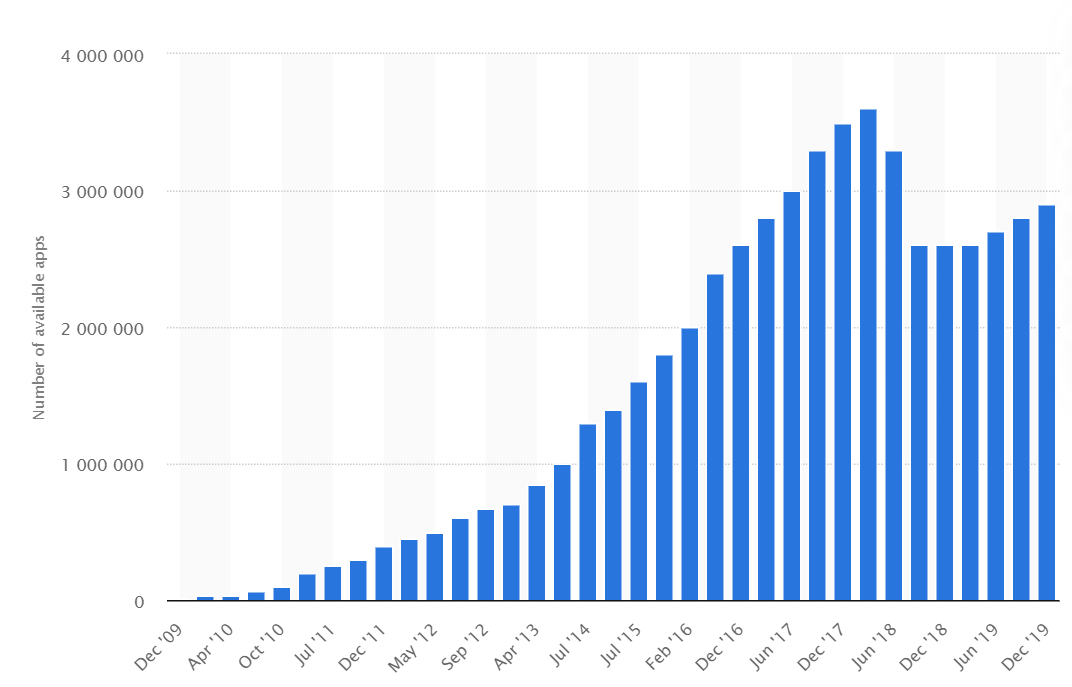
\includegraphics[width=0.9\textwidth]{./Figures/edwin-intro-app-number.png}
	\caption{Google Play 应用商店架上应用总数变化趋势}
	\label{fig:app_number}
\end{figure}

随着Android移动应用行业快速发展,移动黑灰产\footnote{即移动端黑色产业与灰色产业,下文同}也逐渐活跃。
黑灰产是以侵害用户、原应用作者或其他第三方利益为手段,凭此或通过其他可疑方式牟利的产业。
一方面,随着开发移动应用的门槛逐渐下降,开发一个移动应用的成本已经普遍低于开发一个类似的桌面级应用所需的成本~\cite{wasserman2010software};
另一方面,移动应用功能在实现上的灵活性~\cite{storydroid}增加了移动应用的复杂度,针对黑灰产的分析与拦截面临着多重新挑战。
两方面结合,为黑灰色应用进入移动端发展提供了良好的基础。

仿冒应用就是一类广泛存在的移动灰黑产产物。
本文研究的仿冒应用指代开发者根据市面上热门应用的外观仿制的Android应用。
据日常观察,仿冒应用中常有恶意广告弹窗、信息窃取、恶意扣费等行为,开发者可在用户使用仿冒应用时利用广告流量或非法获得的用户信息获利。
一方面,仿冒应用损害了原版应用开发者的知识产权,侵害了原开发者的利益;
另一方面,仿冒应用中的恶意行为也在威胁普通用户的信息安全。
可以联想如下场景:用户尝试通过应用市场搜索安装一个应用,应用市场返回了多个无论是名字或是图标都十分相像的结果,在未有明确指引的情况下,用户安装了仿冒应用。
前人针对Android恶意应用的研究~\cite{Zhou2012DissectingAM}显示,恶意行为可被自动触发,若用户下载的仿冒应用中包含此类恶意行为,用户数据安全将受到损害;
同时,由于用户不能分辨原版应用与仿冒应用,后者的不良用户体验会导致用户对前者乃至应用市场产生不良评价;
即使用户删除仿冒应用、装上原版应用,也浪费了时间和人力成本。

综上所述,仿冒应用影响用户搜索与下载应用时的安全和体验,最终使用户、原版应用开发者和应用市场三方利益均受到损害。
为了消除仿冒应用带来的隐患,无论是开发者、应用市场或是普通用户,都应对仿冒应用的特征与行为有所了解。

\section{研究现状}
尽管客观上存在对仿冒应用进行了解的需求,本研究对移动应用领域的前期调研显示,针对仿冒应用进行的实证研究尚缺乏,也未有公开可用的仿冒应用数据集。
因此,本节讨论与仿冒应用同属于移动灰黑产的重打包应用和恶意应用、以及其他移动应用领域相关方向的研究现状。

\subsection{重打包应用的研究现状}
\label{sec:repackaging}
重打包指恶意开发者对原应用解包、篡改内容之后再将应用重新打包的技术~\cite{khanmohammadi2019empirical}。
重打包应用侵害了应用原作者的知识产权,甚至可能具有恶意行为,因此也属于移动黑灰产范畴。
目前针对重打包应用的相关工作分为三类,分别为关于重打包的实证研究、针对重打包应用的检测和防止应用被重打包的研究。

相关实证研究方面,Khanmohammadi等人对重打包应用进行了一次详尽的实证研究~\cite{khanmohammadi2019empirical}。
该实证研究利用已有数据集AndroZoo~\cite{li2017androzoo++},得出了``重打包应用的主要目的为利用广告获得收入''的结论,并回答了包括``何种类型的应用会被重打包''、``重打包对原应用属性更改如何''在内的五个研究问题,增进了研究者对重打包应用的理解。


在重打包应用检测方面,早期工作通过比对两两应用之间的信息获得应用之间的相似度。
有研究者基于应用指令序列的方法使用模糊哈希的方法提取出应用的摘要信息,如DroidMOSS和DroidAnalytics~\cite{DroidMOSS, Zheng2013DroidAnalyticsA};
也有使用静态数据依赖构建程序依赖图(Program Dependency Graph, PDG)比对应用的方法,如DNADroid~\cite{DNADroid}和AnDarwin~\cite{AnDarwin},Centroid~\cite{Centroid}甚至为应用中的每个函数构建了三维控制流图(3-Dimensional Control Flow Graph, 3D-CFG),将三维控制流图聚合后,通过检测不同应用在控制图聚合后的质心位置判断应用间的相似程度;
还有算法通过比对抽象语义树检测重打包应用,如Hanna等人的Juxtapp~\cite{hanna2012juxtapp}利用K-gram模型对应用的二进制操作码序列进行比对,CLANdroid~\cite{CLANdroid}通过分析五种语义特征点(比如代码中的标识符和调用到的Android API等),以检测相似应用。
上述算法一来因为需要使用静态分析方法对代码进行解析,在遇到使用过代码混淆处理(如反射和代码加密)的应用时性能往往较差;二来需要基于两两比对进行检测,复杂度较高,在应用规模增大时会导致庞大的计算量。
为处理静态分析带来的问题,有学者提出了利用动态分析比对应用的方法,如Wu等人使用HTTP流量对应用行为进行建模~\cite{wu2015detect}。
亦有研究使用信息可视化方法检测重打包应用:ViewDroid~\cite{ViewDroid}通过重建和比对应用的视图筛出重打包应用,DroidEagle~\cite{sun2015droideagle}则利用UI布局相似性检测,Kywe等人比对应用中的文本与图像相似性以寻找相似应用~\cite{kywe2014detecting},Soh等人分析应用运行时收集的UI信息以检测重打包行为~\cite{soh2015detecting}。
而从避免两两比对、减小算法复杂度方面考虑,有学者提出利用第三方库进行检测的办法,如CodeMatch~\cite{CodeMatch}筛选出应用中使用的第三方库代码后,计算并比对剩余部分代码的哈希值,获取不同应用的相似程度;Wukong~\cite{Wukong}也分两步检测重打包应用,但与CodeMatch相比,其第二步使用了基于计数的代码克隆检测手段,而非基于哈希的技术。

防止应用被重打包的研究多基于检测原有代码是否被更改而开展。
Zhou等人提出了两个基于改版Dalvik虚拟机的对抗工具:其中,AppInk~\cite{zhou2013appink}利用一种``水印''技术(Watermarking)对抗重打包,但需要利用一个改版的Dalvik虚拟机进行文件检查;另一工具DIVILAR~\cite{zhou2014divilar}为应用的Dalvik代码提出了一种新编码形式,同时也需要修改用户设备Android系统中的Dalvik虚拟机以对新的编码进行解码。
Luo等人提出了在代码中注入大量检测节点的方法对抗重打包,并推荐开发者进行代码混淆,以避免令重打包开发者发现注入的检测节点~\cite{luo2016repackage}。
与之相似,Zeng等人也提出了在代码中注入逻辑炸弹的方法,并在研究中讨论了多种避免重打包开发者发现代码注入的策略~\cite{zeng2018resilient}。

\subsection{恶意应用的研究现状}
针对恶意应用的研究可分为两个方面,分别是面向恶意应用进行实证研究工作与面向恶意应用检测的研究。

面向恶意应用的实证研究众多,较有代表性的有以下两篇文献:
Felt等人的研究~\cite{Felt2011ASO}仔细剖析了来自多个不同平台的46个恶意程序样本以了解这些样本的激励机制,揭示了这些样本的运行机制和行为策略,为后人抵御此类恶意行为提供参考;
Zhou和Jiang~\cite{Zhou2012DissectingAM}搜集了来自多个主要恶意应用家族的、超过1,200个恶意应用样本,并系统性地描绘了这批样本的不同性质,包括其安装手段、激活机制和其如何执行有效负载(实现恶意行为)。
虽然恶意应用与仿冒应用有重合之处,但两者有一定区别,相关理论知识直接套用并不合适。

以上述实证研究与数据分析作为基础,研究者对恶意应用有了较好的了解,从而得以有针对性地进行恶意应用检测。
相关方法可大致分为静态分析、动态分析与机器学习三个方向。
早期研究通过静态分析手段对恶意应用进行检测,包括Enck等人提出的Kirin,在应用安装时检测应用权限,从而拦截恶意应用的安装~\cite{enck2009lightweight};
Felt等人提出的Stowaway~\cite{felt2011android}利用API调用分析和权限分析,寻找权限过大(Overprivileged)的应用;
RiskRanker~\cite{grace2012riskranker}则提出了一个两阶恶意应用检测手段,先筛选出具有root行为和可能导致隐私泄露的应用,再找出其中具有危险Dalvik代码加载行为的应用。
然而,受静态分析方法本身的限制,此类研究在遇到代码混淆时多被影响性能。
因此,有研究者利用动态分析技术对恶意应用进行检测。
TaintDroid~\cite{enck2014taintdroid}和DroidScope~\cite{yan2012droidscope}均在沙箱中对应用行为进行监视,TaintDroid利用污点分析技术寻找应用的信息泄露行为,DroidScope则从Android系统的不同层面分析应用的可疑行为。
Zhou等人\cite{zhou2012hey}提出了DroidRanger,利用应用行为比对与动态加载分析的方式,成功地从5个应用市场的204,040个应用中找出了211个恶意应用。
ParanoidAndroid~\cite{portokalidis2010paranoid}提出了将恶意检测方法迁移到云端的概念,将设备上的所有操作同步到云端服务器,从而在不影响设备本地功能的情况下进行恶意行为检测。
无论是静态分析方法或是动态分析方法,都需要人工对恶意行为的模式进行描绘,而用人工手段提取行为模式,不仅对领域知识有较高要求,还往往是费力费时的。
针对此问题,研究者开始利用机器学习技术检测恶意应用。
Chen等人从大规模数据集中总结出了恶意应用的两类特征,再将其用于分类器模型训练,提出了检测工具StormDroid~\cite{chen2016stormdroid},与之类似的方法还有CrowDroid~\cite{burguera2011crowdroid},DroidMat~\cite{wu2012droidmat},Adagio~\cite{gascon2013structural},MAST~\cite{chakradeo2013mast},DroidAPIMiner~\cite{aafer2013droidapiminer}与Drebin~\cite{arp2014drebin}。

\subsection{其他相关研究}
Andow等人针对灰色应用的研究~\cite{Andow2016ASO}从Google Play应用商店中采集了多个应用样本。
该研究将样本分类,定义了高仿应用(Imposter)、移动广告应用(Madware)等9种不同的灰色应用。
灰色应用指不具有明显恶意行为,但应用意图存疑、又或是会向系统申请过多权限的应用程序。
因此,这类应用不是恶意应用,但由于其盈利方式可疑,可将其归入移动黑灰产内。

另一方面,Hu等人针对市面上的欺诈约会应用进行了一次实证研究~\cite{hu2019dating}。
该研究中的欺诈约会应用声称自己为约会应用,实则诱导用户开通会员服务,也应归入黑灰产应用范畴。
分析发现,用户在此类应用中遇到的其他``用户''多数不由真人控制,而是具有预设对话模板的聊天机器人。
此外,研究还分析了该类应用的商业模式与分发渠道,评估了受害者的数量,对此类应用的生态进行了详尽解读。
该研究还通过直接检测相同评论和标记可疑用户的方式对此类应用进行排名欺诈检测。

Chen等人发布了漏洞检测工具Ausera~\cite{chen2018ausera},该工具通过静态分析技术与敏感词识别,对手机银行应用进行自动化三段式风险评估。
同期,他们在一个实证研究中利用Ausera从693个手机银行应用中检出超过两千个漏洞,向对应的60家银行发送了漏洞报告,并检查了新发行的手机银行应用以跟进漏洞修补进程~\cite{chen2018mobile}。
在被检出漏洞的60家银行中,21家确认了该研究反馈的漏洞,进行了对应修复,作者随后根据修复状况进行案例研究,分别面向银行、学者与政府,共给出了9条用于改善手机银行应用安全性与市场环境的实用建议。
与之类似,本研究也从多个方面出发,提出了防范仿冒应用、净化市场环境的实用建议。

% \subsection{针对应用评论的相关研究现状}
% 近年来,除了利用应用程序牟利以外,移动黑灰产业也开始进入应用市场评论的领域。
% 相关工作也可以分为检测与相关的实证研究两类。

% 检测方面,
% Zhu等人提出了一个利用评价历史记录检测应用是否具有排名欺诈行为的研究~\cite{zhu2014discovery}。
% 该研究提出,一般应用的排名在上升期(Raising phrase)和下降期(Recession phrase)之间会有一段维持期(Maintaining phrase),维持期过短且排名在短时间内剧烈波动的应用很可能具有排名欺诈行为。
% 然而,用该方法进行检测需要持续收集应用在市场上的评分数据,因此对数据采集有一定要求。
% Lim等人分析了差评水军(Review spammers)的特征并将其用于建模,以检测类似行为~\cite{lim2010detecting};
% Xie等人利用图论挖掘评论中开展共谋攻击(Collusion attack)的用户群组~\cite{xie2014grouptie},并在后续研究中将该方法拓展成一个检测系统~\cite{xie2016you}。
% 与之相似,Chen等人同样使用了基于图论的方法检测共谋攻击~\cite{chen2017toward},
% Hooi等人的FRAUDAR通过寻找二分图中的密集子图寻找关系特别密切的用户与应用,从而找出可能提供排名欺诈服务的可疑用户与使用了该服务的应用~\cite{hooi2016fraudar}。

% 实证研究方面,Rahman等人对Google Play中虚假评论行为的实证研究~\cite{rahman2019art}在公开确认该产业链存在的同时,也揭露了该产业的行为模式、生存情况甚至从业人员收入水平等方面的信息。

% 作为黑灰色产业链下游环节,虚假应用评论(即排名欺诈行为)已在前述研究中被证明与欺诈约会应用存在关联。
% 因此,排名欺诈也很可能与仿冒应用相结合,为移动黑灰产从业者牟取更多利益,有必要开展相关分析进行确认。

\subsection{研究现状小结}
综合上述分析,与仿冒应用同属黑灰产的重打包应用和恶意应用,甚至是日常生活中常用的手机银行类应用,均有对应研究可提供参考。
前人的实证研究收集了较为大量的重打包应用、恶意应用和手机银行应用数据,并提供了重打包应用与原版差异、恶意应用传播方式与负载执行方式、手机银行应用常见漏洞等指导性信息,帮助专业人员改善现有移动应用环境。
在丰富的前序研究提供的领域知识与数据支持下,各界才得以对重打包应用、恶意应用开展后续的检测研究。
相比之下,仿冒应用的相关数据和研究成果都乏善可陈。

换言之,在上述研究中,无论是对恶意应用还是重打包应用进行检测,都需要有一定领域知识或洞见(Insight)作为理论支撑。
对仿冒应用而言,学术界与工业界对其认知均较贫乏,``基于新见解进行技术拓展改良''式的研究手段尚未适用于仿冒应用。
因此,着眼于领域知识梳理的实证研究更适用于仿冒应用在当下的研究场景。
% \subsection{实证研究}
% 实证研究是一种基本研究技术,旨在针对特定方法在实际应用场景下的真实状况或对应产物进行数据收集、调查与分析,以让研究者了解事物的工作原理或使理论得以验证。
%
% 在软件工程领域,由于理论研究与工程实践结合较为紧密,学者采用需要检验理论在实践中的落地情况(如程序语言提供的特性是否被良好地理解与使用~\cite{bieman1995reuse}、是否在工程实践中体现优势等~\cite{harrison2000experimental}问题)或是调研现实应用场景中产生的现象(如恶意应用、重打包应用等在移动端市场出现的实际问题~\cite{Felt2011ASO, Zhou2012DissectingAM, Andow2016ASO, wang2018android}),实证研究技术是十分适合的方法。
% 因此,有越来越多的研究者使用实证研究技术对研究主体进行探索\cite{Felt2011ASO, Zhou2012DissectingAM, Andow2016ASO, wang2018android, chen2018ausera, chen2018mobile, bieman1995reuse, harrison2000experimental, dybaa2008empirical, manotas2016empirical, mcintosh2016empirical, mcilroy2016fresh, wu2016ji, yang2015xin, hu2019dating, khanmohammadi2019empirical}。
% 随着实证研究技术在软件工程领域中的认可度逐渐提高,软件工程顶级会议FSE与ICSE近年分别新设立了面向工业界的投稿分区,鼓励学者多基于应用场景进行实证研究,探明业界现状。
%
% 为向软件工程领域进行实证研究的学者提供方法论支持,Kitchenham等人基于自身在评阅软件工程项目的经验和一份针对医学研究者的研究指引,总结出了一份对于软件工程实证研究的初步准则(Preliminary guideline)~\cite{kitchenham2002preliminary},对实证研究的数据收集方法、实验设置方法等各个步骤都给出了严格指引,如在数据收集时需要确保数据的准确性与完整性,需要保证实验的可重复性等。
% 为保证数据的准确性与完整性,本研究利用\mytool 尽可能全面地收集多个来源的应用样本。
% Seaman则结合实例,提供定性分析的~\cite{seaman1999qualitative}。
% 在实证研究可采取的具体方式方面,Easterbrook等人于2008年提出了面向软件工程领域的实证研究方法建议~\cite{easterbrook2008selecting},为软工实证研究提供方法论参考,文中将实证研究方法论分为受控实验、案例分析、调查研究、社会学意义研究与混合方法途径等多类,以适用于不同场景。
% 本研究采取了其中的案例分析方法。
%
% 前期调研显示,针对仿冒应用进行的实证研究尚缺乏,也没有公开可用的仿冒应用数据集。

\section{拟采用的研究方法}
上述研究现状说明,实证研究在多个研究方向上提供了研究数据或领域知识,有一定实用价值。
当下的仿冒应用研究,既缺乏可用的数据集,也缺乏对应的基本特征知识。
作为基于数据采集和数据分析的技术,实证研究方法正好可缓解仿冒应用领域知识和数据集的缺失,是适用于本课题的技术手段。
本研究将采用实证研究方法,对仿冒应用进行研究。

实证研究是一种基本研究技术,旨在针对特定方法在实际应用场景下的真实状况或对应产物进行数据收集、调查与分析,以让研究者了解事物的工作原理或使理论得以验证,其中数据收集是十分重要的一部分。
前人总结~\cite{kitchenham2002preliminary}对实证研究的数据收集方法给出了严格指引,指出数据收集时需要确保数据的准确性与全面性。
因此,科学地进行数据收集是本研究面临的一个关键问题。

% \section{问题分析与研究难点}
% 前文的研究现状,反映出移动应用领域是目前的研究热点之一,也反映出移动黑灰产无孔不入的特点。
% 为了保障正当开发者的利益与消费者的权益,学术界和工业界都需要对移动黑灰产有更全面、更深入的理解,从而更好地预防未知的威胁。
% 上述研究现状表明,工业界与学术界的软件工程、安全领域在移动应用的研究上已经取得了丰富的成果。
% 然而,现有研究提供的知识仍有空缺部分,移动黑灰产的仿冒应用部分正是缺口之一。
% 在仿冒应用相关研究缺失的情况下,仿冒应用数据严重匮乏,造成了以下问题:
%
% 1)\	\emph{无法对仿冒应用进行定量分析} \quad
% 目前,学术界与工业界目前对恶意应用和排名欺诈行为均有良好理解,厂家得以在实践中抵御、规避此类移动黑灰产的侵袭,这得益于前人在实证调查研究~\cite{Felt2011ASO, Zhou2012DissectingAM, zhou2012hey, rahman2019art}中提供的数据与洞见(Insight)。
% 然而,在仿冒应用数据缺失的情况下,相关定量分析与定性分析无法进行,无法让学术界与工业界对仿冒应用有清楚了解。
% 针对仿冒应用进行实证研究可以有效解决这个问题。
% 具体而言,研究者可从工业界环境(即各应用市场)中获取大量应用,从所获应用中筛选出一定数量的仿冒应用,提取出其中可用于定量分析的数据,从而开展相关分析。
%
% 2)\	\emph{无法确定仿冒应用的性质} \quad
% 尽管仿冒应用在日常生活中随处可见,却少有研究者对其进行研究。
% 因而,仿冒应用的形态尚未明确,亦从未有前人评估仿冒应用的风险性;总结仿冒应用的发展趋势不明,无法确定这一移动黑灰产是否会更加壮大;仿冒应用的市场反馈无人探索,仿冒应用是否会与其他黑灰产业环节结合更是不得而知。
% 针对以上疑问,研究者可采用实证研究的混合方法途径方法论可以通过对数据定性分析,帮助理解仿冒应用具有的性质;而相对的案例分析(Case studies)方法论~\cite{easterbrook2008selecting}则可以在案例支持下更有力地确认定性分析的发现。
%
% 综上,现时仿冒应用数据匮乏、对仿冒应用了解缺失的问题,可通过实证研究缓解。
% 因此,本文与犇众信息的移动安全威胁数据平台Janus~\cite{janus}合作,搜集并分析了大量应用样本,从仿冒应用特征解读和仿冒应用评论分析两方面进行了大规模实证研究,对仿冒应用作出了较为全面的剖析,填补了本领域的研究空白。
% 仿冒应用特征解读利用数据挖掘分析技巧,利用本研究收集到的仿冒应用数据对仿冒应用进行画像,为多方受众提供可借鉴的结论;
% 仿冒应用评论分析则通过收集仿冒应用在市场上获得的反馈,验证仿冒应用和排名欺诈行为的关系,进一步地提供了关于仿冒应用生态的信息。
%
% 在实证研究中,研究者通常都会遇到几点挑战:如何确定研究主体、如何收集数据、如何对数据进行有效处理;
% 而在排名欺诈相关研究中,如何从评论数据中有效挖掘排名欺诈行为是研究者经常要思考的问题。
% 故本实证研究中的难点可概括如下:
%
% 1)\	\emph{如何确定仿冒应用} \quad
% 仿冒应用和正版应用是相对的概念。
% 本文选择了市面上最热门的50个应用,再搜集其对应的仿冒应用样本。
% 从应用中筛选出与热门应用外观相似或是相同的样本后,本文使用Android本身自带的证书机制,将获得样本的证书信息与原版应用的证书信息进行比对,从而鉴别出仿冒的样本。
%
% 2)\	\emph{如何获得针对仿冒应用的大量数据} \quad
% 数据搜集是科研工作中公认的难点。
% 本文想要提供一次全面的研究结果,除了搜集的目标应用需要有多样性之外,也必须获得不同应用市场上的数据,增加研究的代表性。
% 前文提及犇众信息的移动安全威胁数据平台Janus是一个数据整合平台。该平台每天从各大Android应用市场爬取应用样本入库,免去了要针对各个市场重新定制爬虫代码的麻烦。
% 通过设计和实现仿冒应用收集框架\mytool,本文顺利从Janus搜寻到了近14万条数据条目作为原始数据,其中每条数据条目代表Janus从应用市场上获得的一个应用样本。
%
% 3)\	\emph{如何对大量的数据进行有效处理} \quad
% 数据规模和处理效率一直是一对矛盾。
% 由于一条数据条目代表一个应用样本,要对所有应用样本进行详尽分析,明显太耗费时间成本与计算成本;然而,如果只对样本进行简单处理,获得的分析结果就不够全面和深入。
% 在尽量确保分析全面性的前提下,对于每个样本,本研究只抽取8个关键信息项进行分析,以节省时间与计算成本。
%
% 4)\ \emph{如何挖掘评论中的排名欺诈行为} \quad
% 现有的排名欺诈挖掘工作均具有其各自的局限性,或是对评分数据有连续收集要求,或是要求检测者有已知的排名欺诈群体,并不能直接应用到本研究收集的数据中。
% 为此,本研究先后设计了基于用户行为可信度和基于评论内容重复度的两个方法。
% 前者规避了现有方法的局限性,后者进一步解决了大数据量带来的大运算量问题。

\section{本文拟解决的关键问题}
上一节提及,科学地进行数据收集是本研究面临的一个关键问题。
此外,本研究还有两个关键问题,一并列举如下:

\begin{itemize}
	\setlength{\itemsep}{1pt}
	      \setlength{\parskip}{0pt}
	      \setlength{\parsep}{0pt}
	\item \emph{如何科学地获取针对仿冒应用的数据?} \quad
	      由于仿冒应用数据缺失,本文只能自行收集数据。
	      数据搜集是科研工作中公认的难点,为提供一次全面的研究结果,除了数据需要有一定规模以外,搜集的目标应用也需要具备多样性,此外还必须获得不同应用市场上的数据,增加研究的代表性。
	      为此,如何获得大量真实、有效、全面而有代表性的数据将是本文研究的一个关键点。

	\item \emph{如何对仿冒应用进行理解?} \quad
	      仿冒应用虽然普遍存在于各大应用市场中,但尚未有研究对其进行分析,无论是应用市场、研究者还是用户,都缺乏对仿冒应用的理解。
	      为能较全面地认识仿冒应用,需要从不同角度对其进行解读。
	      因此,从应用基本属性、应用作者行为等多角度对仿冒应用进行解析,是本文研究的重点之一。

	\item \emph{是否能有效地筛选仿冒应用} \quad
	      根据日常经验不难发现,在现阶段,用户在实际使用中经常能搜索到仿冒应用,应用市场对仿冒应用的筛选排除并未完善。
	      恶意应用、重打包应用的研究发展表明,充分认识移动黑灰产应用特征对后续的对应检测、发现有明显促进作用。
	      同理,作者希望可基于对仿冒应用进行的解读与画像,设计有效流程帮助各大市场梳理、排除仿冒应用。
	      这是本文研究的另一重点,也是本文的创新点。
\end{itemize}

\section{本文主要工作}
为解决上述三个关键问题,本研究完成了如下主要工作:

\begin{itemize}
	\setlength{\itemsep}{1pt}
	      \setlength{\parskip}{0pt}
	      \setlength{\parsep}{0pt}
	\item \emph{全面的数据集整理} \quad
	      借助自行实现的仿冒应用收集框架,本研究尽可能全面地收集了来自29个应用来源的约14万个应用样本,并从中筛选出5万个仿冒样本,整理成已知的首个仿冒应用数据集,以供其后的相关研究使用。

	\item \emph{仿冒应用数据画像与现实案例分析} \quad
	      本文从基本信息与开发者行为两个方向入手分别进行了实证研究,前者对仿冒引用进行了较为全面的数据画像,后者根据仿冒应用开发者行为推断出现有应用市场监管不足之处。
	      两组研究除了从较高维度进行数据分析外,还从数据集中挑选出应用和证书实例,分别展开案例讨论,以深化在数据画像和行为分析中得到的领域知识。

	\item \emph{提供实用建议} \quad
	      基于在实证研究中的发现,本文分析了仿冒应用特征的可能成因与现有应用市场的不足之处,由此分别面向普通用户、应用市场和相关从业者提供了实用建议。

	\item \emph{基于规则的仿冒应用检测框架} \quad
	      依靠前序研究中对仿冒应用的理解与解读,作者设计并实现了基于规则的仿冒应用检测框架\mytool 。

\end{itemize}

% 现有的排名欺诈挖掘工作均具有其各自的局限性,或是对评分数据有连续收集要求,或是要求检测者有已知的排名欺诈群体,并不能直接应用到本研究收集的数据中。
% 为此,本研究先后设计了基于用户行为可信度和基于评论内容重复度的两个方法。
% 前者规避了现有方法的局限性,后者进一步解决了大数据量带来的大运算量问题。

% \section{研究方法与工作概览}
%
% \subsection{研究方法}
% 前文已经提及,实证研究能够为研究主体提供画像与洞见,从而为对应方面的后续实践与研究提供建议与便利。
% 在软件工程领域与安全领域,已有多篇实证研究~\cite{Felt2011ASO, Zhou2012DissectingAM, Andow2016ASO, wang2018android, chen2018ausera, chen2018mobile, bieman1995reuse, harrison2000experimental, dybaa2008empirical, manotas2016empirical, mcintosh2016empirical, mcilroy2016fresh, wu2016ji, yang2015xin, hu2019dating, khanmohammadi2019empirical}为实践工作提供知识支持。
% 因此,本文亦将采用实证研究方式,对仿冒应用进行探索。
%
% 与相关文献~\cite{easterbrook2008selecting}提供的方法结合,本文研究中使用到的是案例分析方法。
% % 1)\ \emph{混合方法途径(Mixed-method approaches)} \quad
% % 混合方法途径指结合定量分析与定性分析,对研究对象进行系统数据解读的实证研究方法。
% % 按照实施的方式,混合方法途径可分为顺序解释策略(Sequential explanatory strategy)、顺序探索策略(Sequential exploratory strategy)与并发三角策略(Concurrent triangular strategy)三类。
% % 顺序解释策略先收集与分析定量数据,再收集和分析定性数据,以定性数据结果帮助解释定量结果;与之相反,顺序探索策略先收集与分析定性数据,再收集和分析定量数据,以定量数据结果帮助解释定性结果;并发三角策略则会同时采用不同方法,以试图确认、交叉验证或证实已有发现。
% % 本文的特征解读部分先采用定量分析方法分析数据,再采用案例分析方法给出定性结果,使用了顺序解释策略;而后续的仿冒应用与排名欺诈关联验证先给出定性结论,再提供定量数据支持,则使用了顺序探索策略。
% % \emph{案例分析(Case studies)} \quad
% 案例分析是软件工程领域最常用的实证研究方法,完整的案例分析通过确立研究问题、选择研究案例和收集数据三步研究真实场景中出现的现象,适用于真实环境为对研究主体产生影响的因素之一、又或是实验数据时间跨度较大的场景。
% 对于针对某些现象的初步调查,可使用探索性案例分析(Exploratory case studies)以提出新猜想和构建理论;而验证性案例分析(Confirmatory case studies)则用于验证现存理论。
% 本文的案例分析既包含用于提出新猜想的探索性案例分析,亦包含验证数据画像的验证性案例分析。
%
% \subsection{工作概览}
%
% \begin{figure}[htbp]
% 	\centering
% 	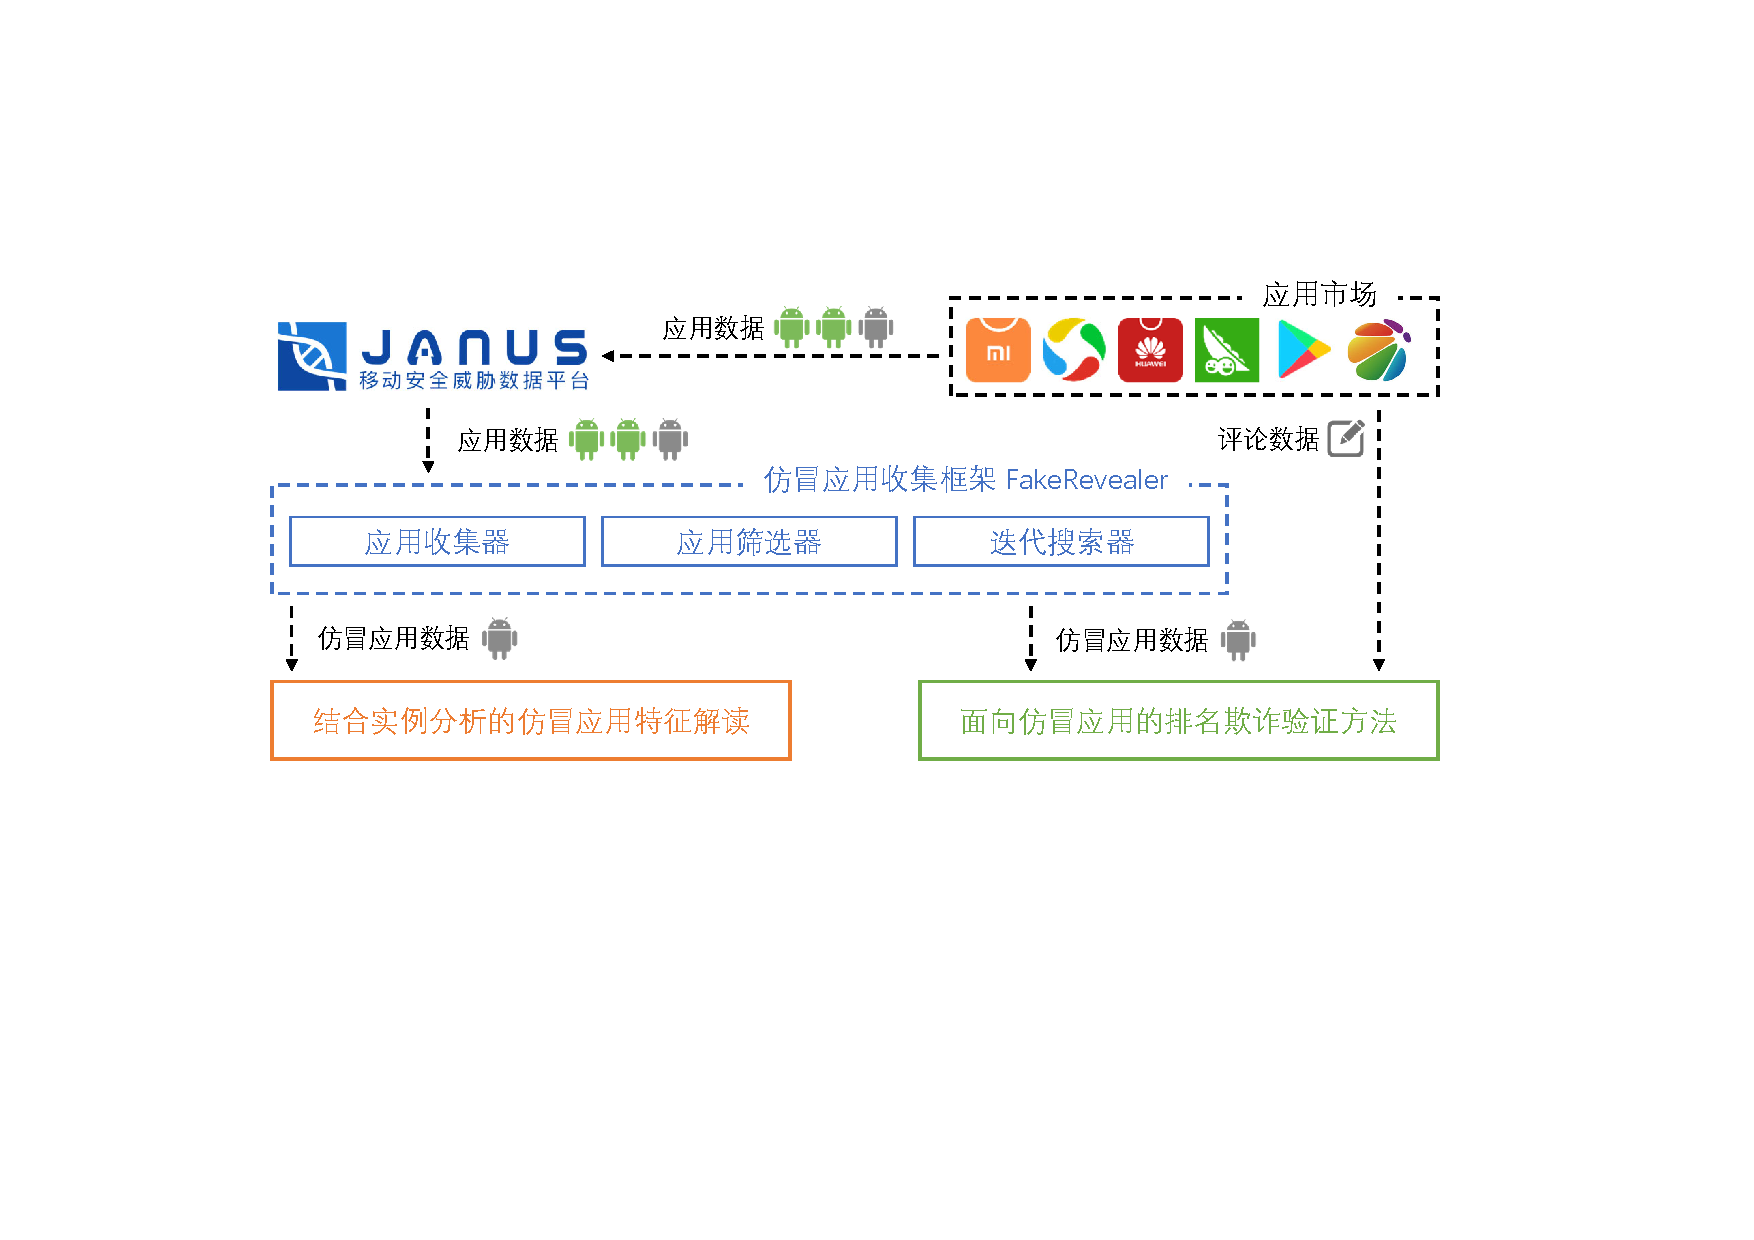
\includegraphics[width=\textwidth]{./Figures/edwin-overview}
% 	\caption{本文工作概览}
% 	\label{fig:Workflow}
% 	\vspace{-3mm}
% \end{figure}
%
% 本节为本文工作提供概览。如\autoref{fig:Workflow}所示,本工作通过三个主要部分,完成三部分工作:
%
% 1)\ \emph{利用面向仿冒应用的收集框架\mytool 收集大规模数据,解决仿冒应用数据稀缺的问题} \quad
% 针对实证研究中实验数据应尽可能具有完整性与代表性的要求,本研究设计并实现了仿冒应用收集框架\mytool,尽可能全面地进行仿冒应用的数据收集。
% 数据收集主要分为两个部分:正版应用信息的收集和仿冒应用的收集。
% 在正版应用信息收集的部分,本文选择了50个最热门的App作为目标应用,然后手动收集了跟这些App有关的信息;
% 基于该50款目标应用,本研究利用\mytool,收集了从29个应用来源获得的近14万个应用样本,并从中筛选出5万个仿冒应用,整理成集。
% 该数据集可为后续相关工作如代码分析、特征检测等提供数据支持。
%
% 2)\ \emph{首次针对仿冒应用的特性进行大规模的特征解读} \quad
% 针对移动黑灰产研究中关于仿冒应用的研究空白,本研究利用上述仿冒应用数据,结合案例分析,进行了首次基于Android系统仿冒应用的大规模特征解读。
% 特征解读从三个视角完成,这些视角分别是仿冒的基本应用特征、影响仿冒应用数量的因素和仿冒应用的发展轨迹,由浅入深揭示仿冒应用的生态。
% 对应的三个案例分析除了为特征解读提供案例支持之外,还揭示了更多仿冒应用开发者的行为特征,可为用户、应用市场和安全领域从业人员等多方受众提供一定见解。
%
% 3)\ \emph{面向仿冒应用的排名欺诈验证} \quad
% 该部分中,本文从第三方应用市场中随机选取一部分应用,爬取用户对它们的所有历史评价,以检测仿冒应用与排名欺诈行为的关联。
% 针对前人检测研究需要先验知识或特殊数据的问题,本研究从社交媒体研究引入了用户行为可信度进行排查,避开了现有方法的局限性。
% 进一步地,本研究从评论内容重复率方面提出了另一创新性排查方法,解决了数据量增大带来的大运算量问题。
% 人工复查结果显示,两种排查方法均取得了优于现有方法的结果。
\section{本文组织结构}
% todo: 7 chapters?
本文共分为七章,环绕着本研究的数据搜集和不同的分析方向展开,各章节内容如下:

\fullref{chp:intro} 主要提供了本文的研究背景、相关工作、本文拟采用的研究方法、拟解决的问题与本文的主要工作。

\fullref{chp:background} 介绍相关技术背景,从软件工程领域的实证研究出发,介绍实证研究的常用方法和数据收集、验证标准等理论背景,再着眼于本研究的主体——Android应用,介绍了Android安全证书机制和与仿冒应用相关的重打包技术。

\fullref{chp:research_settings} 介绍整个研究的设置,包括根据研究现状提出研究问题、确立研究对象,阐述数据收集的相关考量,并与其他研究收集的数据进行对比。

\fullref{chp:discoveries_basic} 从仿冒应用与原版应用相似度、影响应用被仿冒的严重程度的因素及仿冒应用行为三点入手,对与仿冒应用基本特征相关的三个方面进行实证研究,最后针对研究结果分别向用户、应用市场和应用开发者提供实用建议。

\fullref{chp:discoveries_behavior} 则结合应用证书视角与结合时间维度视角进行探索,分析现有应用市场监管策略存在的不足,针对性地提出改善措施。

\fullref{chp:framework_prototype} 提出了一个基于规则的仿冒应用检测框架,并将前两章实证研究所得的经验总结为规则,对框架进行了有效性检验。

% % 这些视角包括仿冒应用特征、影响仿冒应用数量的因素和仿冒应用的发展轨迹,每个视角都被进一步分解成多个不同的研究问题。
% % 说明仿冒应用的数据收集方式并详细介绍其中三个组件(\componentA、\componentB 和\componentC)的设计与实现,
% % 结束解读后,本文从数据中挑选三个具有代表性的案例进行分析,以案例进一步深化分析结果。

% \fullref{chp:feedback} 针对仿冒应用进行了排名欺诈检测。
% 针对现有检测方法的不足,本文先后提出两个具有创新性的方法对排名欺诈行为进行排查,并将排查结果与前一章的仿冒应用进行比对。
% % 结果显示,仿冒应用存在排名欺诈行为。仿冒应用与排名欺诈行为作为移动黑灰产的两个环节存在关联。

\fullref{chp:future} 对本文工作进行总结,并对下一步工作进行展望。

\clearPaperPage

\chapter{Android背景介绍}
\label{chp:background}

本章主要介绍Android系统、Android应用程序和应用市场相关的背景知识,包括现有的Google Play市场和多个第三方市场共存的局面介绍,同时也会介绍Android安全证书机制的相关背景。

\section{Android系统介绍}
Android系统是属于Google公司的开源操作系统,基于Linux内核研发。
其最早版本于2008年发布(Android 1.0),起先只针对手机端发布。
由于具有图形化操作界面,并且采用触屏作为交互方式,极其简单易用,Android系统自发布起就迅速在智能手机领域抢占大量市场份额,搭载Android系统的平板电脑也在我们的日常生活中渐渐变得随处可见。
近年来,随着IoT(Internet of Things,物联网)的发展,家用电器趋向智能化,不少电视厂商、机顶盒厂商、甚至可穿戴设备厂商也开始为产品内嵌深度定制的Android系统,为用户提供更好的体验。

\begin{figure}[htbp]
	\centering
	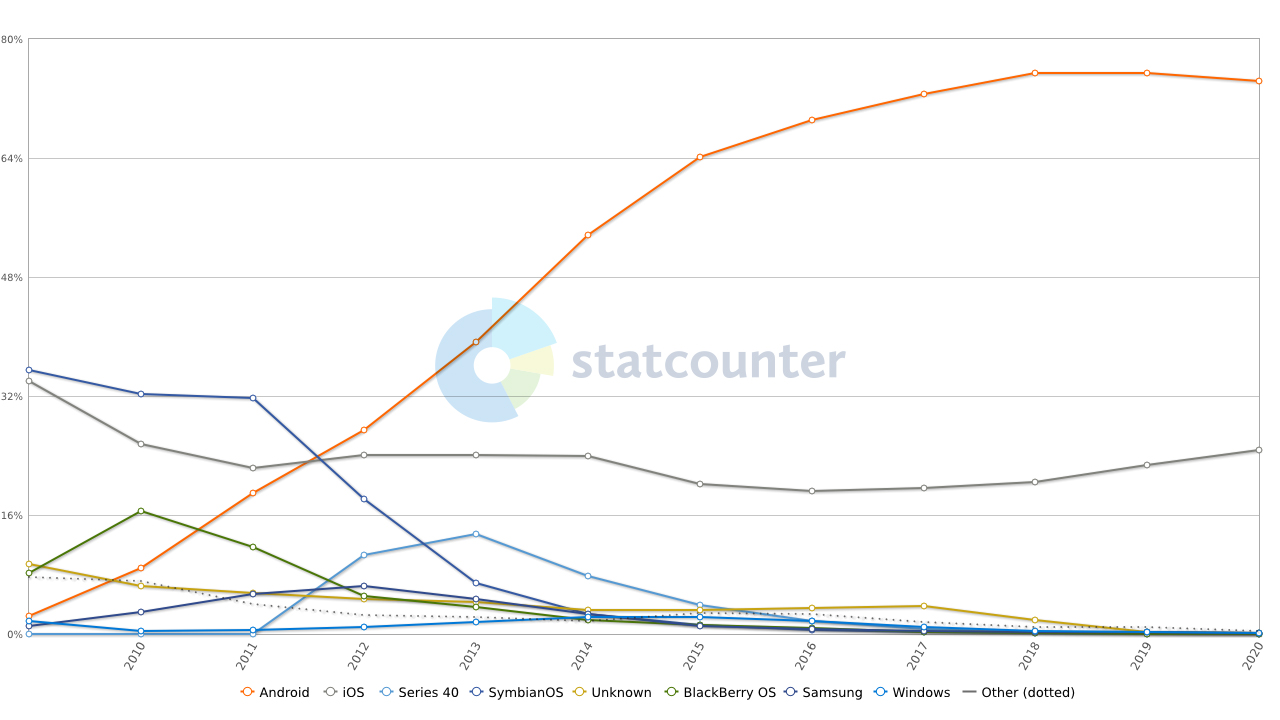
\includegraphics[width=0.95\textwidth]{./Figures/edwin-StatCounter-os-mkt-share-yearly-2009-2020.jpg}
	\caption{2009至2020年移动端操作系统市场份额变化图}
	\label{fig:Android-Mkt-Share}
	\vspace{-5mm}
\end{figure}

图~\ref{fig:Android-Mkt-Share}展现了2009年到2020年间不同移动端操作系统对市场占有率的变化曲线,图表来源于数据分析机构StatCounter~\cite{MobileOSMktShare},图表X轴为时间线,Y轴为市场份额占总量的百分比。
不同颜色的曲线代表不同操作系统,其中Android系统由橘红色曲线表示。
从图中数据可知,自发布以来,Android系统便一路高歌猛进,迅速占据移动端操作系统市场,从2012年起就获得了业界第一的市场份额占有率,直到2020年,其超过70\%的市场占有率依然遥遥领先于其他操作系统。
其中原因,除了对用户非常友好的操作方式以外,也在于其具有一个多元、开放又充满活力的应用程序生态环境。

\section{Android应用程序}

\subsection{应用程序简介}

Android应用程序(Android Application,简称App)是可以安装在Android系统上、拓展系统功能的软件,这些软件通常基于Java语言开发,其中可以包含用C语言或者C++编写的库以提高性能。
2014年起,Google宣布Android支持Kotlin编程语言,自此开发者也可以使用Kotlin语言进行Android App开发。

Android App的开发需要使用Google提供的软件开发工具包(Software Develop Kit,简称SDK)和Google支持的集成开发环境(Integrated Development Environment,简称IDE)。
SDK是包含了众多软件包的工具箱,其中有包括了Android系统应用程序接口(Application Programming Interface,简称API)的函数库和用以编译App的各种工具,在编译完成之后,开发者还可以利用SDK的相应工具为App签上自己的数字签名。
API函数库提供了Android系统的一系列接口,开发者需要在使用Android App框架的前提下,调用各种API实现自己设计的功能。

在发布每一版本Android系统的同时,Google公司也会发布一个新版本的Android SDK供开发者开发App。
每个人都可以从Android的官方网站上下载Android SDK和开发应用所需的IDE,这意味着,利用官方发布的工具,任何人都可以开发出属于自己的Android App。

\subsection{构建应用程序}

与大部分软件一样,开发者在发布自己的App之前,也先需要把代码编译打包成Android操作系统使用的一种应用程序包格式文件APK(Android application package)。
每个APK文件都会包含该款App的一系列基本信息,包括App的应用名、包名(Package name)、安全证书等。
其中,包名是Android系统识别App的依据,每款App在不同的版本可以有不同的应用名,但其包名必须是一致的。
图~\ref{fig:Android-Build-Process}展现了APK文件的构建流程。
一般来说,一个Android App的构建流程会分为以下四步,整个构建流程由Android SDK中的Android插件和Gradle构建工具管理。

\begin{figure}[htbp]
	\centering
	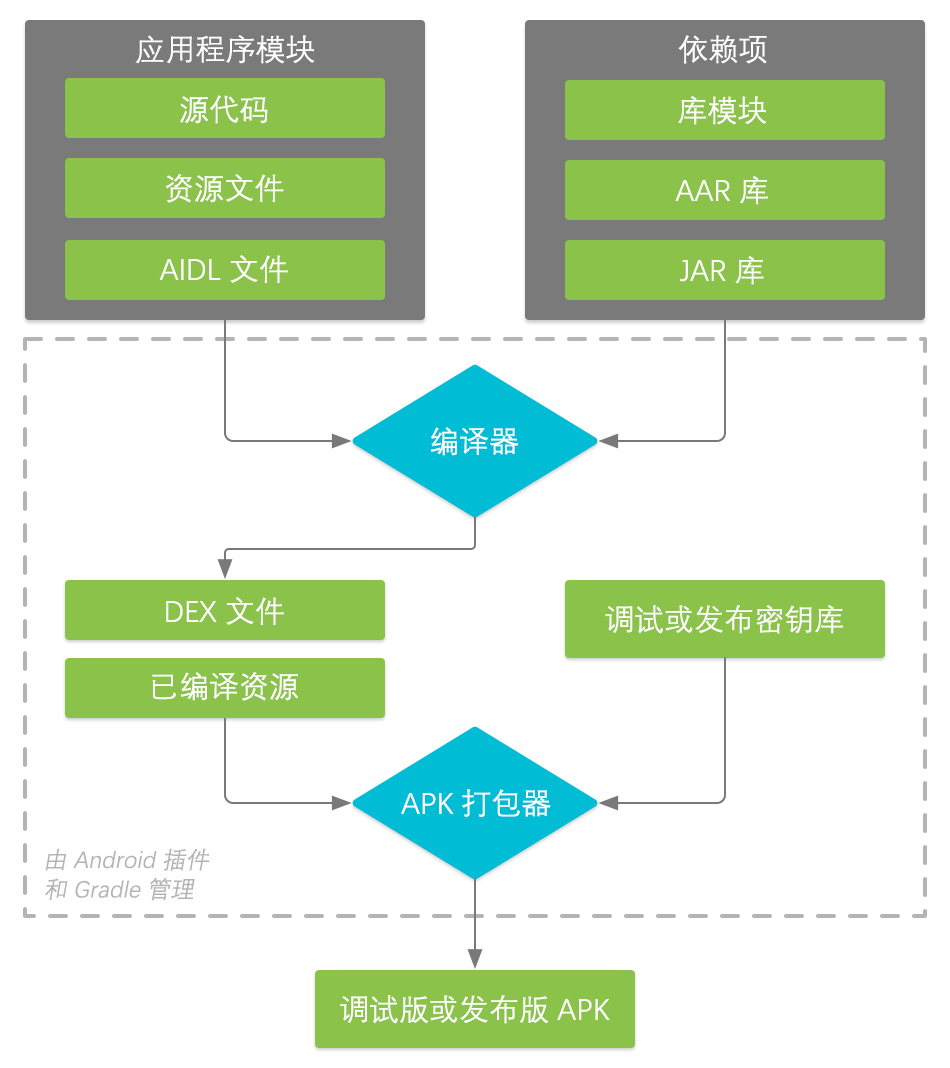
\includegraphics[width=0.6\textwidth]{./Figures/edwin-build-process-CHN.png}
	\caption{Android App构建流程}
	\label{fig:Android-Build-Process}
\end{figure}

首先,开发者需要编写App对应的源代码,然后连同一些源代码中使用到的依赖项一起输入到编译器中生成DEX文件。
源代码可以由Java语言或者Kotlin语言编写,而DEX文件则是一种可执行文件,可以运行于Dalvik虚拟机上。
Dalvik虚拟机则是Android系统的核心组成部分之一,用于运行被编译为DEX文件的程序。
此外,编译器还会将其他未被编译的资源文件转换为编译后的资源。

然后,SDK中的APK打包器会将DEX文件和已经编译好的资源文件一起打包。
APK文件的本质是压缩文件,其中包含了被编译的代码文件、App需要用到的资源文件(比如字符串、图片等资源)、assets资源、App的安全证书和Manifest配置文件,所以APK打包器的任务是将这些所有文件都压缩进一个APK文件里面。
不过,在这个步骤,APK打包器还未将所有文件压缩。
因为在压缩之前,还需要进行下一步的签名。

在第三步,APK打包器会使用密钥库文件对上一步中提及的资源文件和代码文件进行数字签名。
这个步骤是用作校验APK文件是否被篡改、保证APK文件完整性的一个重要步骤,在本章后续内容中会有相关机制的更多介绍。

最后,APK打包器会使用zipalign工具对应用进行优化,以减少App在设备上运行时所占用的内存。
这步结束之后,整个构建流程也随之结束。
开发者会获得一个编译好、签名完毕并且经过优化的APK压缩文件,然后就可以将这个APK文件安装到Android设备上运行使用。


\section{Android应用市场}
由于每个人都可以开发、构建自己的Android App,从网上发布的App数不胜数。这种开放性为Android应用生态带来开放性的同时,也会引入以下几个问题:

1)\ \emph{难以择优} \quad
开放的环境会导致App数量难以胜数。由于从互联网上找到的App质量良莠不齐,用户有时无法判断网上的应用是否符合自己的需求;

2)\ \emph{数据安全} \quad
智能手机与现代人的日常生活息息相关,其中也自然包含了各人的隐私数据甚至财产信息。确保用户下载、安装到的应用不会损害到他们的财产安全和数据安全至关重要;

3)\ \emph{宣传渠道} \quad
开发者希望自己的App尽可能地受欢迎,但中小开发者并没有足够的资源去宣传自己的应用,可能会导致原本质量优秀的App因为缺少宣传渠道而无人问津;

4)\ \emph{收入结算} \quad
开发者有从App中获得盈利的需求。即使是部分出于兴趣或其他非盈利目的开发手机应用的开发者,也需要从App中获取补贴以维持App的维护和正常运作。如何利用App变现、变现之后又要怎样将资金回流到开发者的问题有待解决;

5)\ \emph{应用更新} \quad
随着时间推进,用户的需求并非一成不变,开发者也需要针对App中以往出现的漏洞查漏补缺、或者更新软件功能,但要求用户定期/不定期地手动更新某个App甚至多个App并不现实。

Google发布的应用商店Google Play~\cite{GooglePlay}的存在缓解了以上的问题。它是Android操作系统的官方应用商店,可以让用户浏览和下载商店中的App。
一方面,普通用户可以经由Android系统中预装好的Google Play服务寻找、购买和下载心仪的App;另一方面,Google Play也允许开发者将App通过开发者账户上传到Google Play中,在经过一系列的审查之后上架到商场上供用户下载。与上述的五个问题对应,Google Play应用商店提供了以下几点服务:

1)\ \emph{一个由官方背书的下载渠道} \quad
这确保了用户下载的App得到官方认可。同时,Google Play也提供了一个关于App的社区条件,用户可以对App进行打分、评论,用户对App的评价经审核后可以由所有其他用户查看,直接影响其他用户对``是否要下载某款应用''的决定;

2)\ \emph{上架之前的应用审核} \quad
在开发者上传App时对App作出一定的审查,以排除部分恶意开发者在商场中上架病毒和恶意应用的可能性。Google Play也会根据用户反馈、应用本身运营数据等原因于每季度从商店中移除一部分App,以保证商店货架上App的质量;

3)\ \emph{作为激励机制的推荐榜单} \quad
在用户评价的基础上,Google Play筛选出一部分质量优异的App制订出一些推荐榜单。推荐榜单会在应用商店首页进行展示,榜单包括``编辑精选''、``热门应用''、``年度之选''等,其中既有大公司开发的App,也会有中小开发者独立开发的应用。此外,Google还会通过用户的使用习惯、所在地区等因素为用户提供个性化推荐(如图~\ref{fig:Google-Play-Main}所示),在不同的App类别下,也有不同榜单为用户推荐,加大了优秀App的曝光率;

\begin{figure}[htbp]
	\centering
	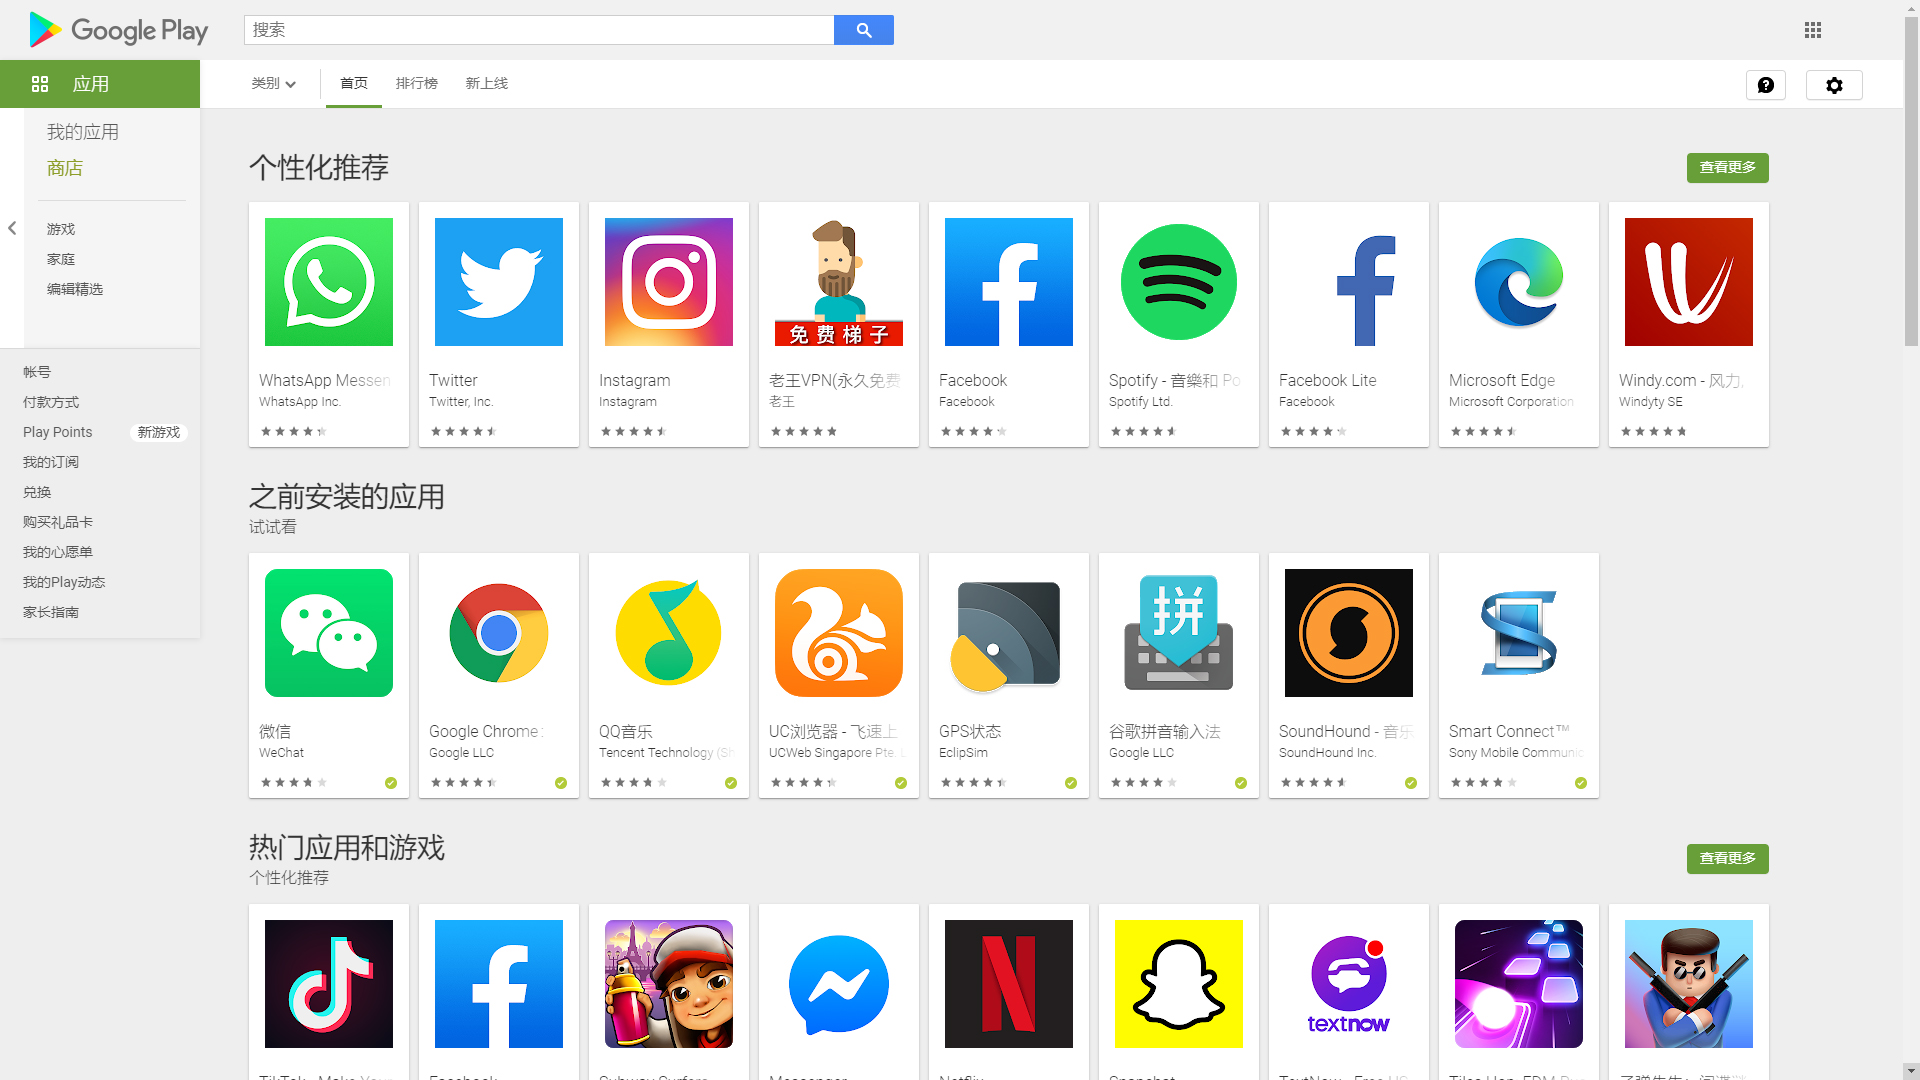
\includegraphics[width=\textwidth]{./Figures/edwin-google-play.jpg}
	\caption{Google Play应用商店首页(从桌面端浏览)}
	\label{fig:Google-Play-Main}
\end{figure}

4)\ \emph{集中的结算通道} \quad
Google Play应用商店为开发者提供了一个统一的结算渠道。应用开发者可以在App内销售商品,然后选择Google Play提供的集成结算服务。用户在购买服务时,直接向Google付款,Google再在每个结算周期将款项结算给开发者。这样一来,开发者尤其是独立开发者就可以更专注于App本身的开发,而不需要考虑如何利用应用变现、再将资金回收的复杂问题。Google Play也允许开发者将自己的App上架为付费应用,需要用户付款后才可下载;

5)\ \emph{方便快捷的更新推送} \quad
由于Google Play本身是个应用程序的集中平台,而且也预置到了大多搭载Android的设备中,所以开发者在更新应用时,只需将新版本上传到Google Play的后台,应用商店经过审核之后,就可以将新版本的应用推送到用户的设备中,让用户设备中的App实现自动更新,免去双方的麻烦。


\section{第三方应用市场}

Google Play应用商店无疑为用户和开发者都提供了一个优良的解决方案,每个应用底下由用户评论组成的社区也促成了用户和开发者之间的交流,用户反馈直接推动了开发者对应用的改良。

遗憾的是,由于种种原因,Google Play应用商店的服务并非对全球的所有地区和国家都开放。
Google从2008年开始退出中国大陆市场,因此Google的大部分服务,包括Google Play应用商店的下载服务在内,都不向中国大陆境内用户提供。
换句话说,国内的大部分普通用户并不能享受到Google Play应用商店的便利。

为此,国内有多家厂商都推出了自己开发的应用市场服务,试图填补这一片市场空白。
实际上,由于整合开发者、用户和App资源三者本身就有巨大的市场潜力,所以即使是在Google Play服务可用的其他国家和地区,也有厂商推出自己的应用市场(如三星推出的三星应用商店、Amazon推出的Amazon应用市场),试着在这个市场上分一杯羹。

纵观国内的应用市场,经过几年的竞争与整合,依然未有出现像Google Play应用商店一样具有垄断性地位的厂商。
多个厂商各据一方,主要可以分为两个类别。
一类是国内IT行业巨头旗下的应用市场,如腾讯旗下的应用宝~\cite{Myapp}和百度旗下的百度应用市场~\cite{Baiduappstore},其平台本身就具有大量基础用户,可以直接转化为应用市场中的活跃用户;另一类则是由各大手机厂商开发的应用市场,如华为的应用市场、小米的小米应用市场~\cite{Xiaomiappstore}等,这类的应用市场通常直接预装在手机出厂时自带的厂家定制Android系统中,凭借手机销量直接带动市场用户增长。

根据数据分析机构艾媒咨询于2018年12月发布的《2018-2019中国中国移动应用商店市场监测报告》~\cite{ChineseAppStoreReport}显示,使用第三方移动应用商店的用户在手机网民中占比为59.99\%。结合国内网民数目庞大的现状,这一数字表示第三方应用市场在国内已被广泛接受。而40.01\%未使用第三方移动应用商店的用户比例则表示这一市场还有广阔前景。该报告还提供了2018年国内第三方应用市场用户首选市场的分布图,如图~\ref{fig:CHN-Mkt-Dist}所示,用户对第三方移动应用市场的选择主要还是集中在国内IT巨头发布的应用市场上。约40\%的手机用户会使用360旗下的360手机助手作为首选应用市场,而首选使用豌豆荚、UC应用商店等阿里应用分发平台旗下应用商店的用户约占11\%。大部分市场份额都已被国内IT巨头旗下的应用市场占领。

\begin{figure}[htbp]
	\centering
	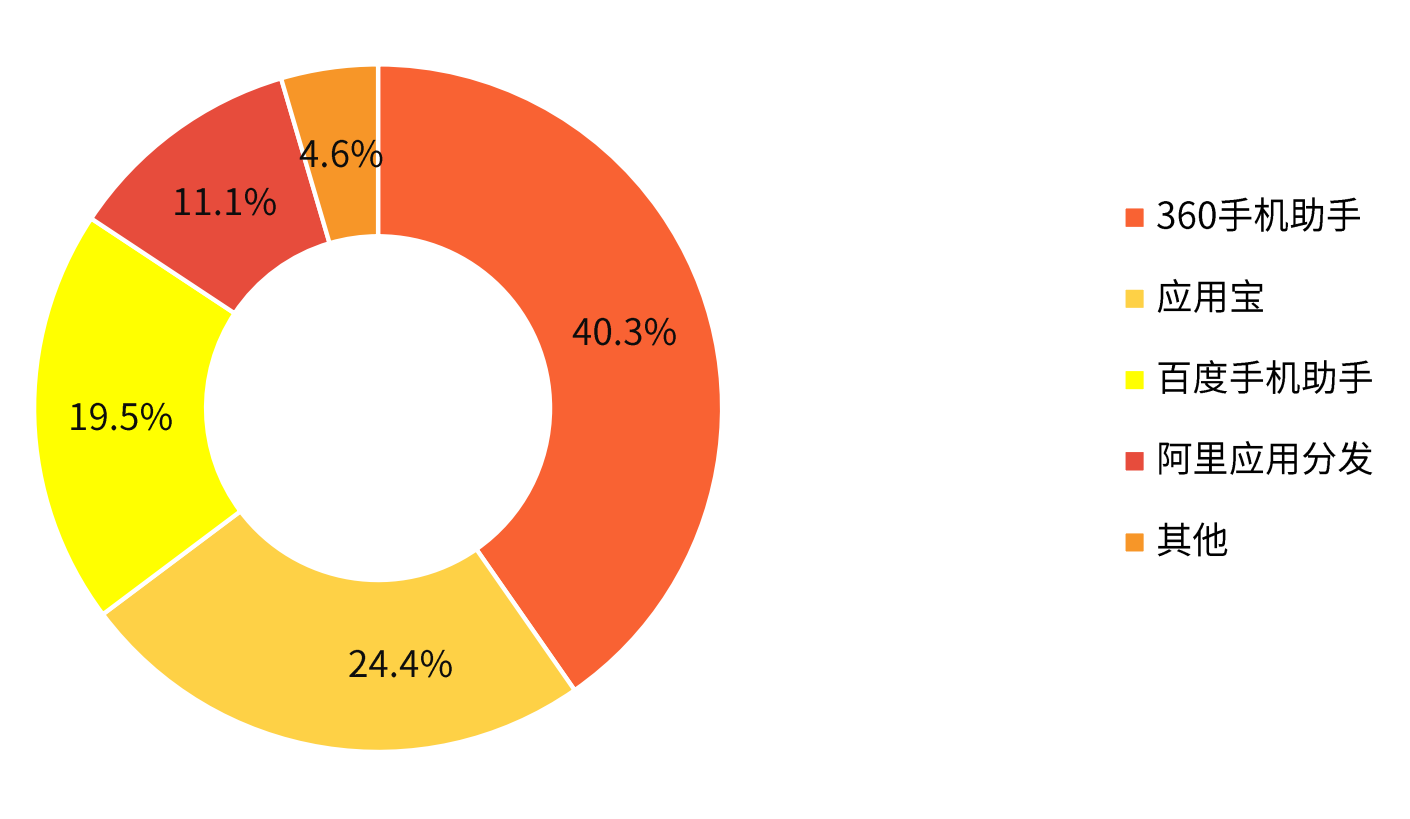
\includegraphics[width=0.5\textwidth]{./Figures/edwin-CHN-mkt-dist.png}
	\caption{2018中国第三方移动应用商店用户首选使用品牌分布}
	\label{fig:CHN-Mkt-Dist}
\end{figure}

与Google Play提供一个完整的Android生态环境相似,上述的各个厂商也致力于构建各自的Android应用生态链条:各大厂商本身就具有一定知名度,从其旗下的应用市场下载应用能让用户放心;开放开发者中心,让开发者注册账号后上传自己制作的App;为每一个App提供评分和评论功能,构建出开发者和用户的交流平台;在应用市场首页设置应用排行榜、推荐安装软件等榜单(如图~\ref{fig:mkt-yyb}),提高优秀App的曝光率;应用市场自带的应用版本管理开发者在市场后台更新应用之后,将更新推送到用户的手机上;各大应用市场也会整合支付平台(如支付宝和微信支付)来应对市场内的应用购买业务,华为应用市场甚至像Google Play一样,为市场上的应用提供了自家的支付渠道以支持应用内的付款项目购买功能。

\begin{figure}[htbp]
	\centering
	
\includegraphics[width=0.8\textwidth]{./Figures/edwin-yyb.jpg}
	\caption{腾讯应用宝应用市场首页(从桌面端浏览)}
	\label{fig:mkt-yyb}
	\vspace{-5mm}
\end{figure}

不同于在Android系统发布早期就存在的Google Play应用商店,国内的第三方应用商店是后期出现的产物,一出现就面临着激烈的市场竞争。
一方面,在国内各类第三方应用市场方兴未艾之时,国内的Android开发者社群尚未成熟,应用市场还未有大量开发者进驻;
另一方面,在成立初期,为了抢占市场份额,各个应用商店都想方设法将商店内App的种类和数量最大化,以迎合市场用户各种各样的需求。
作为结果,各类第三方应用市场都在各个渠道搜集App,而非通过开发者上传的方式获得货架上的应用程序。
由于在早期各种监管渠道尚未完善,各个市场在搜罗各类App的同时,难免会将大量的盗版应用也一并收录。

\section{Android App签名机制}

前文提到,开发者在使用Android SDK构建App时,其中十分重要的一步是对App进行数字签名。
实际上,Android的数字签名和安全证书机制基于RSA公共密钥系统,是Android安全机制中不可或缺的一个部分。
本章的余下内容将会对Android App的签名机制进行简单分析。

Android App的签名机制是用作校验APK文件是否被篡改、保证APK文件完整性的一个重要机制,所有的应用都必须要在经过签名才能安装进Android系统中。
在签名时,SDK会使用一种密钥库文件,如果开发者还没有这个文件的话,SDK会自动生成一个。
密钥库中包含了开发者的各种信息,包括一对公钥和私钥。
私钥用于数字签名,不可向外公布;公钥则是可以向外公布的一组密钥,用于数字前面的验证。
App中的签名也是系统用来识别开发者的重要依据,因为同一个密钥库文件会产生一致的签名,系统能根据签名中的公钥验证应用识别开发者。

签名的过程大致如下:
在前文流程的第二步结束后,编译器会输出DEX文件和编译好的资源文件,这时,SDK会对每个文件都扫描一次,然后对每个文件提取一次数字摘要,再把每个文件的文件名和其对应的数字摘要保存在一个名为\textit{MANIFEST.MF}的文件中。
之后,SDK会再扫描一次刚才生成的\textit{MANIFEST.MF}文件,再次提取一次数字摘要,把这个摘要连同刚才文件中的所有内容存入另一个新文件\textit{CERT.SF}里。
第三步,再计算一次\textit{CERT.SF}的数字摘要,然后用密钥库中的私钥对这个摘要进行加密。
加密后的结果就是数字签名。
最后,SDK将签名、公钥、计算数字摘要的哈希算法等信息写入\textit{CERT.RSA}文件中,再将这整个过程中生成的四个文件放进\textit{META-INF}文件夹,用APK打包器打包起来。
至此流程结束。

而Android系统验证签名的方式,则是先通过\textit{CERT.RSA}中的公钥验证签名是否无误,再根据文件中提供的哈希算法计算APK包中所有文件的数字摘要:先从\textit{CERT.SF}开始,然后是\textit{MANIFEST.MF},然后是APK中的其他所有文件...
一旦其中出现不相符的结果,就会导致验证失败。
在安装App的过程中,验证签名失败会使得系统终止App的安装。

换句话说,在一个APK被打包签名完毕之后,如果需要更改其中的内容,就只能在更改后将APK重新打包签名一次,即使是一个bit的修改也会破坏原有的签名。
这也是系统可以用数字签名识别开发者的原因:签名一致的App,最后一定都是由同一个开发者打包的。
所以,具有同样签名的App也可以在同一个Android设备上共享数据。
不过这超出了本文讨论的内容,故按下不表。

目前,签名的模式共有三代,其区别主要在于构建流程第三、第四步之间的一些操作上。
简单地说,越新的签名模式能越好地保障APK文件的完整性。
实际上,第一代签名模式V1具有较为致命的缺陷,所以Google官方也在呼吁开发者在编译时采用最新的签名模式。

要注意的是,签名机制只能保证APK文件在被篡改之后不能凭借原有的签名被安装进Android系统,但恶意开发者依然可以在篡改APK之后,用自己的密钥库对APK重新签名,构建出可安装的App。
这种App是盗版App的一种,被称为重打包App。

\section{本章小结}

本章主要介绍了Android系统、Android应用和Android应用市场的相关背景知识,同时也阐述了Android应用的构建流程和简要介绍了其中使用到的签名机制,为后文实证研究中使用到的采样来源和验证方法做铺垫。

\clearPaperPage

\chapter{相关概念介绍}
\label{chp:definition}


在本节,我们将给出拓展动态函数调用图构建过程中的基本术语,并基于这些概念定义Android系统中常见的触发关系,结合具体示例进行解释说明。

\section{概念说明}
方法执行是一个方法执行相关信息的描述,方法对象对应是和方法执行相关的对象\footnote{在Java语言中,函数称为方法。在本文中,两者可以相互替换,不做区分。};
调用关系和触发关系描述了方法执行之间的关系。
函数调用图为所有调用关系的集合,在函数调用图上添加和方法相关的对象信息,补全方法间触发关系得到拓展函数调用图。

\subsection{关于方法和对象的定义}

\begin{Def}
	方法对象%(Method Object,MO)
\end{Def}

和方法执行相关的对象称为方法对象,可以体现对象和执行方法的相互关系。
在本文中,方法对象通常用符号$o$表示。
	

	对于方法执行$m$,对象和方法执行的关系(简称为方法对象关系)如下所示:
	\begin{itemize}
%				\setlength{\itemsep}{-5pt}
				\setlength{\itemsep}{1pt}
				\setlength{\parskip}{0pt}
				\setlength{\parsep}{0pt}
		\item 参数关系:若对象$o_p$是这个方法$m$的参数,记为$m \joinrel\xrightarrow{parameter} o_p$;%,或者 $ rel(m,o_p) = parameter$;%,或者三元组$\left\langle m, o_p, parameter\right\rangle $;
		\item 返回值关系:若对象$o_r$是这个方法$m$的返回值,记为$m \joinrel\xrightarrow{return} o_r$;%,或者 $ rel(m,o_r) = return$;%,或者三元组$\left\langle m, o_p, return\right\rangle $;
		\item 实例关系:若方法$m$是非静态方法,则方法执行时我们可以获取到关联到的this指针对象$o_i$,记为$m \joinrel\xrightarrow{instance} o_i$;%,或者 $ rel(m,o_i) = instance$;%,或者三元组$\left\langle m, o_p, instance\right\rangle $;
	\end{itemize}

通常情况下,一个方法执行过程中,返回值对象和实例对象不允许超过一个,而方法参数可以有多个\footnote{返回值为void的方法无返回值对象,静态方法无实例对象。}。
一个对象可以同时是一个方法执行过程中的实例、参数或者返回值,具体情况由函数执行过程决定。



\begin{Def}方法执行\end{Def}

方法执行是对方法执行过程中的相关信息的描述,完整的信息包括对应方法的完整签名、执行时所处的线程以及相关的方法对象。
在本文中,方法执行通常用符号$m$表示。

\subsection{关于方法间关系的定义}
\begin{Def}
	调用关系%(Invoke)
\end{Def}

对于程序$P$的两个方法执行$m_1$和$m_2$,方法$m_1$调用了方法$m_2$,则记作$m_1 \to m_2$,称为方法$m_1$调用方法$m_2$。

\eat{
\begin{equation}
m_0 \to  m_1 \to  \dots \to m_n \to m   ( n \geqslant 0)  
\end{equation}
}


\begin{equation}
m_0 \to  m_1 , m_1 \to  m_2 , \dots , m_n \to m  ( n \geqslant 0)  
 \label{equ:extend_invoke}
\end{equation}

对于方法执行$m$,若存在方法执行$m_i$($i=0,\dots,n , n \geqslant 0$),使得\autoref{equ:extend_invoke}成立,则记作$m_0 \to  m_1 \to  \dots \to m_n \to m$,简写为$m_0 \stackrel{\ast}{\to} m$,称为方法$m_0$扩展调用方法$m_n$。
方法$m_0$扩展调用方法$m$的路径用$\left[ m_0 ,   \dots , m_n , m \right] $ 表示。
特殊的,当$n=0$时,对于方法$m_0$和方法$m$,$m_0 \to m$成立,则$m_0  \stackrel{\ast}{\to}  m$也成立。



\important{在系统源代码的层面上},对于方法$m$和$m'$,若方法$m$的执行过程总是会调用方法$m'$(即$m \to m'$\important{总是}成立),可以记为 $m \Rightarrow m'$;
类似的,若\eat{对于方法$m$和$m'$,}$m  \stackrel{\ast}{\to}  m'$总是成立,可以记为 $m  \stackrel{\ast}{ \Rightarrow } m'$。

\begin{Def}
	触发关系%(Trigger)
\end{Def}
	
	%如果对于动态函数调用图$DCG$中两个方法(不妨记为$m_a$和$m_b$,$m_a \in DCG$,$m_b \in DCG $),
	若方法$m_a$和方法$m_b$之间同时需要满足以下三个条件,
	则两个方法存在触发关系,记为$m_a \hookrightarrow m_b$ 或者$m_{a} \lhook\joinrel\xrightarrow{\text{因果关系}}  m_{b} $,称为$m_a$触发调用$m_b$:
	
	\begin{itemize}
		\setlength{\itemsep}{-5pt}
		\item  方法执行$m_a$的执行时间总是在方法执行$m_b$的执行时间之前;
		\item 方法$m_a$和$m_b$之间不存在一条调用路径,即$m_a \stackrel{\ast}{\to} m_b $不成立;
		\item $m_a$、$m_b$之间存在着因果关系,包括但不限于事件回调或多线程交互等。
	\end{itemize}


以多线程中的Thread为例,方法\code{Thread.start()}(记为$m_{start}$)的执行会使JVM/Dalvik虚拟机创建一个新的线程。
最终,虚拟机会在新的线程中回调该Thread对象的方法\code{Thread.run()}(记为$m_{run}$)。
上述描述可以表示成$m_{start} \hookrightarrow m_{run}$。由于这个触发关系和多线程相关,也可以记作$m_{start} \lhook\joinrel\xrightarrow{Thread}  m_{run} $。
同样的,触发关系也适用于UI事件注册与响应\eat{UI事件注册与响应指的是控件的点击事件,例如\code{View.setOnClickeListener(View\$OnClickListener)}和\code{View\$OnClickListener.onClick(View)}的关系} 、基于Handler的多线程交互。

\important{在系统源代码的层面上},对于方法$m_a$ ,$m_b$ ,$m_c$ ,
若$m_a  \stackrel{\ast}{ \Rightarrow } m_b$ 、 $m_b \hookrightarrow m_c$\important{同时}成立,则$m_a \hookrightarrow m_c$成立;
若$m_a  \hookrightarrow m_b$ 、 $m_b \stackrel{\ast}{ \Rightarrow }  m_c$\important{同时}成立,则$m_a \hookrightarrow m_c$成立。

\subsection{关于调用图的定义}

\begin{Def}
	函数调用图%(CallGraph,CG)
\end{Def}	


	函数调用图是对程序运行时行为的描述,用有向图$CG = ( V , E)$表示。 图中的点和\textbf{方法执行} $m$一一对应;
	如果方法$m_1$调用方法$m_2$(即$m_1 \to m_2$),则有向边 $e = \left\langle m_1  \to m_2 \right\rangle $属于有向边集合 $E$;
	如果方法$m_1$触发方法$m_2$(即$m_1 \hookrightarrow m_2$),则有向边 $e' = \left\langle m_1  \hookrightarrow m_2 \right\rangle $属于有向边集合 $E$。 


\textbf{注意:}
在应用执行过程中,方法A被调用了两次,方法A的每次执行都调用了方法B,则对应的函数调用图$CG$如\autoref{equ:dcg_sample}所示。
在调用图$CG$中,$m_a$ 和 $m_b$ 各有两个,分别对应的两次\textbf{方法执行}。
$\left\langle m_{a_{1}} \to m_{b_{1}}\right\rangle $对应的是第一次函数A调用函数B,
$\left\langle m_{a_{2}} \to m_{b_{2}} \right\rangle    $对应的是第二次函数A调用函数B,

\eat{
\begin{equation}
\begin{aligned}
CG = &(V,E) ,\\ 
V = & \{m_{a_{1}},m_{b_{1}},m_{a_{2}},m_{b_{2}}\}, \\ 
E = & \{  
\left\langle  m_{a_{1}} \to m_{b_{1}} \right\rangle  ,\left\langle  m_{a_{2}} \to m_{b_{2}}\right\rangle 
\} 
\end{aligned}
\end{equation}
}
{ 
\equwuhao


\begin{equation}  
\left\{  
\begin{array}{lll}
CG &= &(V,E) ,\\ 
  V &= & \{m_{a_{1}},m_{b_{1}},m_{a_{2}},m_{b_{2}}\}, \\ 
  E &= & \{  
\left\langle  m_{a_{1}} \to m_{b_{1}} \right\rangle  ,\left\langle  m_{a_{2}} \to m_{b_{2}}\right\rangle 
\}. 
\end{array}  
\right.  
\label{equ:dcg_sample} 
\end{equation} 

}


\begin{Def}
	拓展函数调用图%(Extended CallGraph,ECG)
\end{Def}


	在函数调用图的基础上,添加了方法对象和函数间的触发关系。
	拓展函数调用图中的节点包括方法执行节点和方法对象节点。图中的边包括描述方法间关系的边和描述方法和对象间的边:
	前者的方法间关系包括调用关系和触发关系;而后者的关系包括和方法对象相关的三个关系(即参数关系、返回值关系与实例关系)。
	
\eat{
	具体定义如\autoref{equ:def_edcg}所示:

\begin{equation}
\begin{aligned}
EDCG =              & (V_{EDCG},E_{EDCG}) ,\\ 
DCG =                & (V_{DCG},E_{DCG}) ,\\ 
V_{EDCG} =      & V_{method} \bigcup V_{object} ,\\
V_{method} =   & V_{DCG}, \\ 
G_{EDCG} =      & G_{method} \bigcup G_{object} , \\
G_{method} =  & E_{DCG} \bigcup \{ \left\langle m_1 , m_2 \right\rangle  \mid m_1 \hookrightarrow m_2 \}
\end{aligned}
\label{equ:def_edcg} 
\end{equation}
}
	
	
\section{Android系统中的触发关系}

触发关系描述的是方法执行间的关系。
触发定义通常由对象与方法的属性约束条件和对象与方法的关系约束条件两个部分组成。
前者描述的是对象和方法执行的属性约束条件,即对对象$o$本身的类型$o.class$、定义方法$m$的类$m.class$、方法执行$m$的方法签名$m.sign$和方法执行$m$的方法完整签名$m.methodSign$(即$m.class$和$m.sign$的组合)等属性的约束;
后者对应的则是对象和方法之间的关系,包括方法对象关系、方法间的调用关系。
本文中涉及的触发关系包括以下几种。



\subsection{基于事件响应的触发关系}


Andoid事件回调的触发关系描述的是控件点击事件的注册和响应之间的因果关系,即方法\code{View.setOnClickeListener(View\$OnClickListener)}(用$m_{register}$表示)和\code{View\$OnClickListener.onClick(View)}间的因果关系(用$m_{click}$表示)。
在上述方法中,方法$m_{register}$的实例对象$o_{view}$是方法$m_{click}$的参数对象,而方法$m_{register}$的参数对象$o_{listener}$是方法$m_{click}$的实例对象。
因此,当两个方法$m_{register}$ 、$m_{register}$及其方法对象$o_{view}$、$m_{register}$满足\autoref{equ:rule_ui}时,$m_{register} \lhook\joinrel\xrightarrow{UiEvent}  m_{register}  $ 成立。
%我们观察发现:
%因此,在构建Andoid事件回调的触发关系过程中,当方法$m_{register} $、$m_{click} $满足第19$\sim$22行的条件时,这两个方法之间存在触发关系,即$m_{register} \lhook\joinrel\xrightarrow{UiEvent}  m_{click}  $(第23行)。


{ 
	\equwuhao
\begin{equation}  
\left\{
\begin{array}{ll}
&o_{view}.class =\text{\codeInEqu{View}};\\
& o_{listener}.class  \in  \{ c \mid  c \text{为类\codeInEqu{View\$OnClickListener}  的子类}  \};\\
&m_{register}.methodSign =\text{\codeInEqu{View.setOnClickListener(View\$OnClickListener)}};\\
& m_{click}.class \in  \{ c \mid  c \text{为类\codeInEqu{View\$OnClickListener}  的子类}  \};\\
&m_{click}.sign =\text{\codeInEqu{onClick(View)}};\\
&m_{register}\joinrel\xrightarrow{instance} o_{view}   ,  m_{register} \joinrel\xrightarrow{parameter}   o_{listener};\\
&m_{click} \joinrel\xrightarrow{parameter}   o_{view} ,  m_{click} \joinrel\xrightarrow{instance}   o_{listener}.
%\left\langle m_{register}\joinrel\xrightarrow{instance} o_{view}\right\rangle,\left\langle m_{register} \joinrel\xrightarrow{parameter}   o_{listener}\right\rangle  \in ecg			 \\ 
%\left\langle m_{click} \joinrel\xrightarrow{parameter}   o_{view}\right\rangle,\left\langle m_{click} \joinrel\xrightarrow{instance}   o_{listener}\right\rangle  \in ecg
\end{array}  
\right.  
\label{equ:rule_ui} 
\end{equation}  
}

\subsection{基于Java 多线程交互的触发关系}


基于Java的多线程交互往往是以{Runnable}作为传递对象,通常通过调用方法\code{Thread.start()} (用$m_{start}$表示)和\code{Activity.runOnUiThread(Runnable)}(用$m_{runOnUiThread}$表示)等API,进而触发类{Thread}和{Runnable}的方法\code{run()}(用$m_{run}$表示)的执行。

通过方法$m_{start}$触发方法$m_{run}$的执行时,方法$m_{start}$和$m_{run}$的实例对象均为同一个{Thread}对象$o_{thread}$。
%因此,对于方法,如果存在一个\code{Runnable}类型的对象\code{r},它既是方法$m_{start}$的实例,又是方法$m_{run}$的实例,则两个方法间存在触发关系,即$m_{start} \hookrightarrow m_{run}$。
因此,当两个方法$m_{start}$ 、$m_{run}$及{Thread}对象$o_{thread}$满足\autoref{equ:rule_thread}时,$m_{start} \lhook\joinrel\xrightarrow{Thread}  m_{run}  $ 成立。
{ 
	\equwuhao
\begin{equation}
\left\{  
\begin{array}{ll}
&m_{start}.methodSign  = \text{\codeInEqu{Thread.start()}};\\
&m_{run}.class \in  \{ c \mid c \text{为类\codeInEqu{Thread}的子类} \} ;\\
&m_{run}.sign = \text{\codeInEqu{run()}};\\
&o_{thread} \in  \{  c \mid \text{c为类\codeInEqu{Thread}的子类}  \} ;\\
&m_{start}\joinrel\xrightarrow{instance} o_{thread} , m_{run} \joinrel\xrightarrow{instance}   o_{thread} .
\end{array}  
\right.  
\label{equ:rule_thread} 
\end{equation}
}

同样的,对于方法\code{Activity.runOnUiThread(Runnable)},也存在类似的关系:
在该触发关系中,{Runnable}类型的对象$o_r$,既是方法$m_{runOnUiThread}$的参数,又是方法$m_{run}$的实例。
因此,当两个方法$m_{runOnUiThread}$ 、$m_{run}$及其方法对象$o_{r}$满足\autoref{equ:rule_runOnUiThread}时,$m_{runOnUiThread} \lhook\joinrel\xrightarrow{runOnUiThread}  m_{run}  $ 成立。
{ 
	\equwuhao
\begin{equation}
\left\{  
\begin{array}{ll}
&m_{runOnUiThread}.methodSign = \text{\codeInEqu{Activity.runOnUiThread(Runnable)}};\\
&m_{run}.class \in  \{ c \mid c \text{为接口\codeInEqu{Runnable}的实现类} \} ;\\
& m_{run}.sign = \text{\codeInEqu{run()}};\\
&o_{r}.class\in  \{  c \mid  c \text{为接口\codeInEqu{Runnable}的实现类}  \} ;\\
& m_{runOnUiThread} \joinrel\xrightarrow{parameter}   o_r ,  m_{run} \joinrel\xrightarrow{instance}   o_r  .
\end{array}  
\right.  
\label{equ:rule_runOnUiThread} 
\end{equation}
}

\subsection{基于{Handler} 多线程消息调度的触发关系}

根据第\ref{chp:background}章中关于{Handler}的介绍,我们知道{Handler}通过{Message}进行多线程消息调度:
通过方法\code{enqueueMessage(Message)}(用$m_{enqueue}$表示)向消息队列从放入消息(用$o_m$表示);
通过方法\code{dispatchMessage(Message)}(用$m_{dispatch}$表示)从消息队列中取出消息$o_m$,进行对应业务逻辑处理。
%首先,我们利用类\code{Handler}的方法\code{enqueueMessage(Message)}(用$m_{enqueue}$表示)和\code{dispatchMessage(Message)}(用$m_{dispatch}$表示)公用同一个Message对象的特点,
因此,当两个方法$m_{enqueue}$ 、$m_{dispatch}$及其方法对象$o_{m}$满足\autoref{equ:rule_handler}时,$m_{enqueue} \lhook\joinrel\xrightarrow{Handler}  m_{dispatch}  $ 成立。
{ 
	\equwuhao
\begin{equation}
\left\{  
\begin{array}{ll}
&m_{enqueue}.methodSign = \text{\codeInEqu{Handler.enqueueMessage(Message)}};\\
&m_{dispatch}.methodSign = \text{\codeInEqu{Handler.dispatchMessage(Message)}};\\
& o_m.class =   \text{\codeInEqu{Message}}; \\
 &m_{enqueue}\joinrel\xrightarrow{parameter} o_m  , m_{dispatch}\joinrel\xrightarrow{parameter} o_m.
\end{array}  
\right.  
\label{equ:rule_handler} 
\end{equation}
}

\section{举例说明}



以第\ref{chp:background}章中的\autoref{fig:handler-code}为例,我们将简要阐述上述概念。
在线程WorkerThread中,方法\code{run()}\eat{$m_{run}$}依次调用了方法\code{Message.obtain()}(用$m_{obtain}$表示)和方法\code{Handler.sendMessage(Message)}(用$m_{send}$表示),则有$m_{run} \to m_{obtain} $和$m_{run} \to m_{send}$。
对于方法$m_{ontain}$,$o_{m} \joinrel\xrightarrow{return} m_{obtain} $成立。
对于方法$m_{send}$,$o_{m} \joinrel\xrightarrow{parameter} m_{send} $、$o_{handler} \joinrel\xrightarrow{instance} m_{send} $成立。
%在Handler的方法handleMessage(Message)中,则有$m_handle \to $
通过对Android Handler 运行机制的分析,我们知道$m_{enqueue} \hookrightarrow m_{dispatch}$。
从\autoref{fig:handler-apis}、\autoref{fig:handler-framework}中可知,所有的Handler API最后就会调用到\code{Handler.enqueueMessage( MessageQueue, Message, long)}方法,即$m_{send} \stackrel{\ast	}{\Rightarrow} m_{enqueue} $,以及$m_{dispatch} \stackrel{\ast}{\Rightarrow}  m_{handle}$,
因此,方法$m_{send}$ 触发调用了方法$m_{handle}$ ,即$m_{send} \hookrightarrow m_{handle}$或$m_{send} \lhook\joinrel\xrightarrow{Handler}  m_{handle} $。

\section{本章总结}

本章介绍了本文使用到的基本概念,从方法和对象的关系、方法间关系、调用图等几个方面对方法关系、方法执行、调用关系、触发关系、函数调用图、拓展调用图等概念做了符号化的定义。
在此基础上,本章从对象与方法的属性约束条件、对象与方法的关系约束条件两个方面对Android系统中的触发关系做了详细的定义。
同时,本章还结合第二章的Handler例子简单阐述了上述概念。

\clearPaperPage

\chapter{RunDroid的系统设计}
\label{chp:design}





本文提出了一个可用于还原Android应用程序运行时动态函数调用图的系统——RunDroid。
RunDroid利用源程序代码插桩和运行时方法拦截的相结合的方式,捕获应用程序在应用层面和系统层面的方法执行信息,还原方法间的调用关系。
在此基础上,RunDroid利用对象和方法的关系结合具体的触发规则,进而还原出方法间触发关系,在调用图中展现运行过程中的Android特性行为。
RunDroid提供的函数调用图从方法调用关系、方法间的触发关系以及方法执行的相关对象信息等多个方面较为全面地刻画了Android应用程序的执行过程。


\section{整体设计}



\begin{figure*}[!ht]
	\centering
	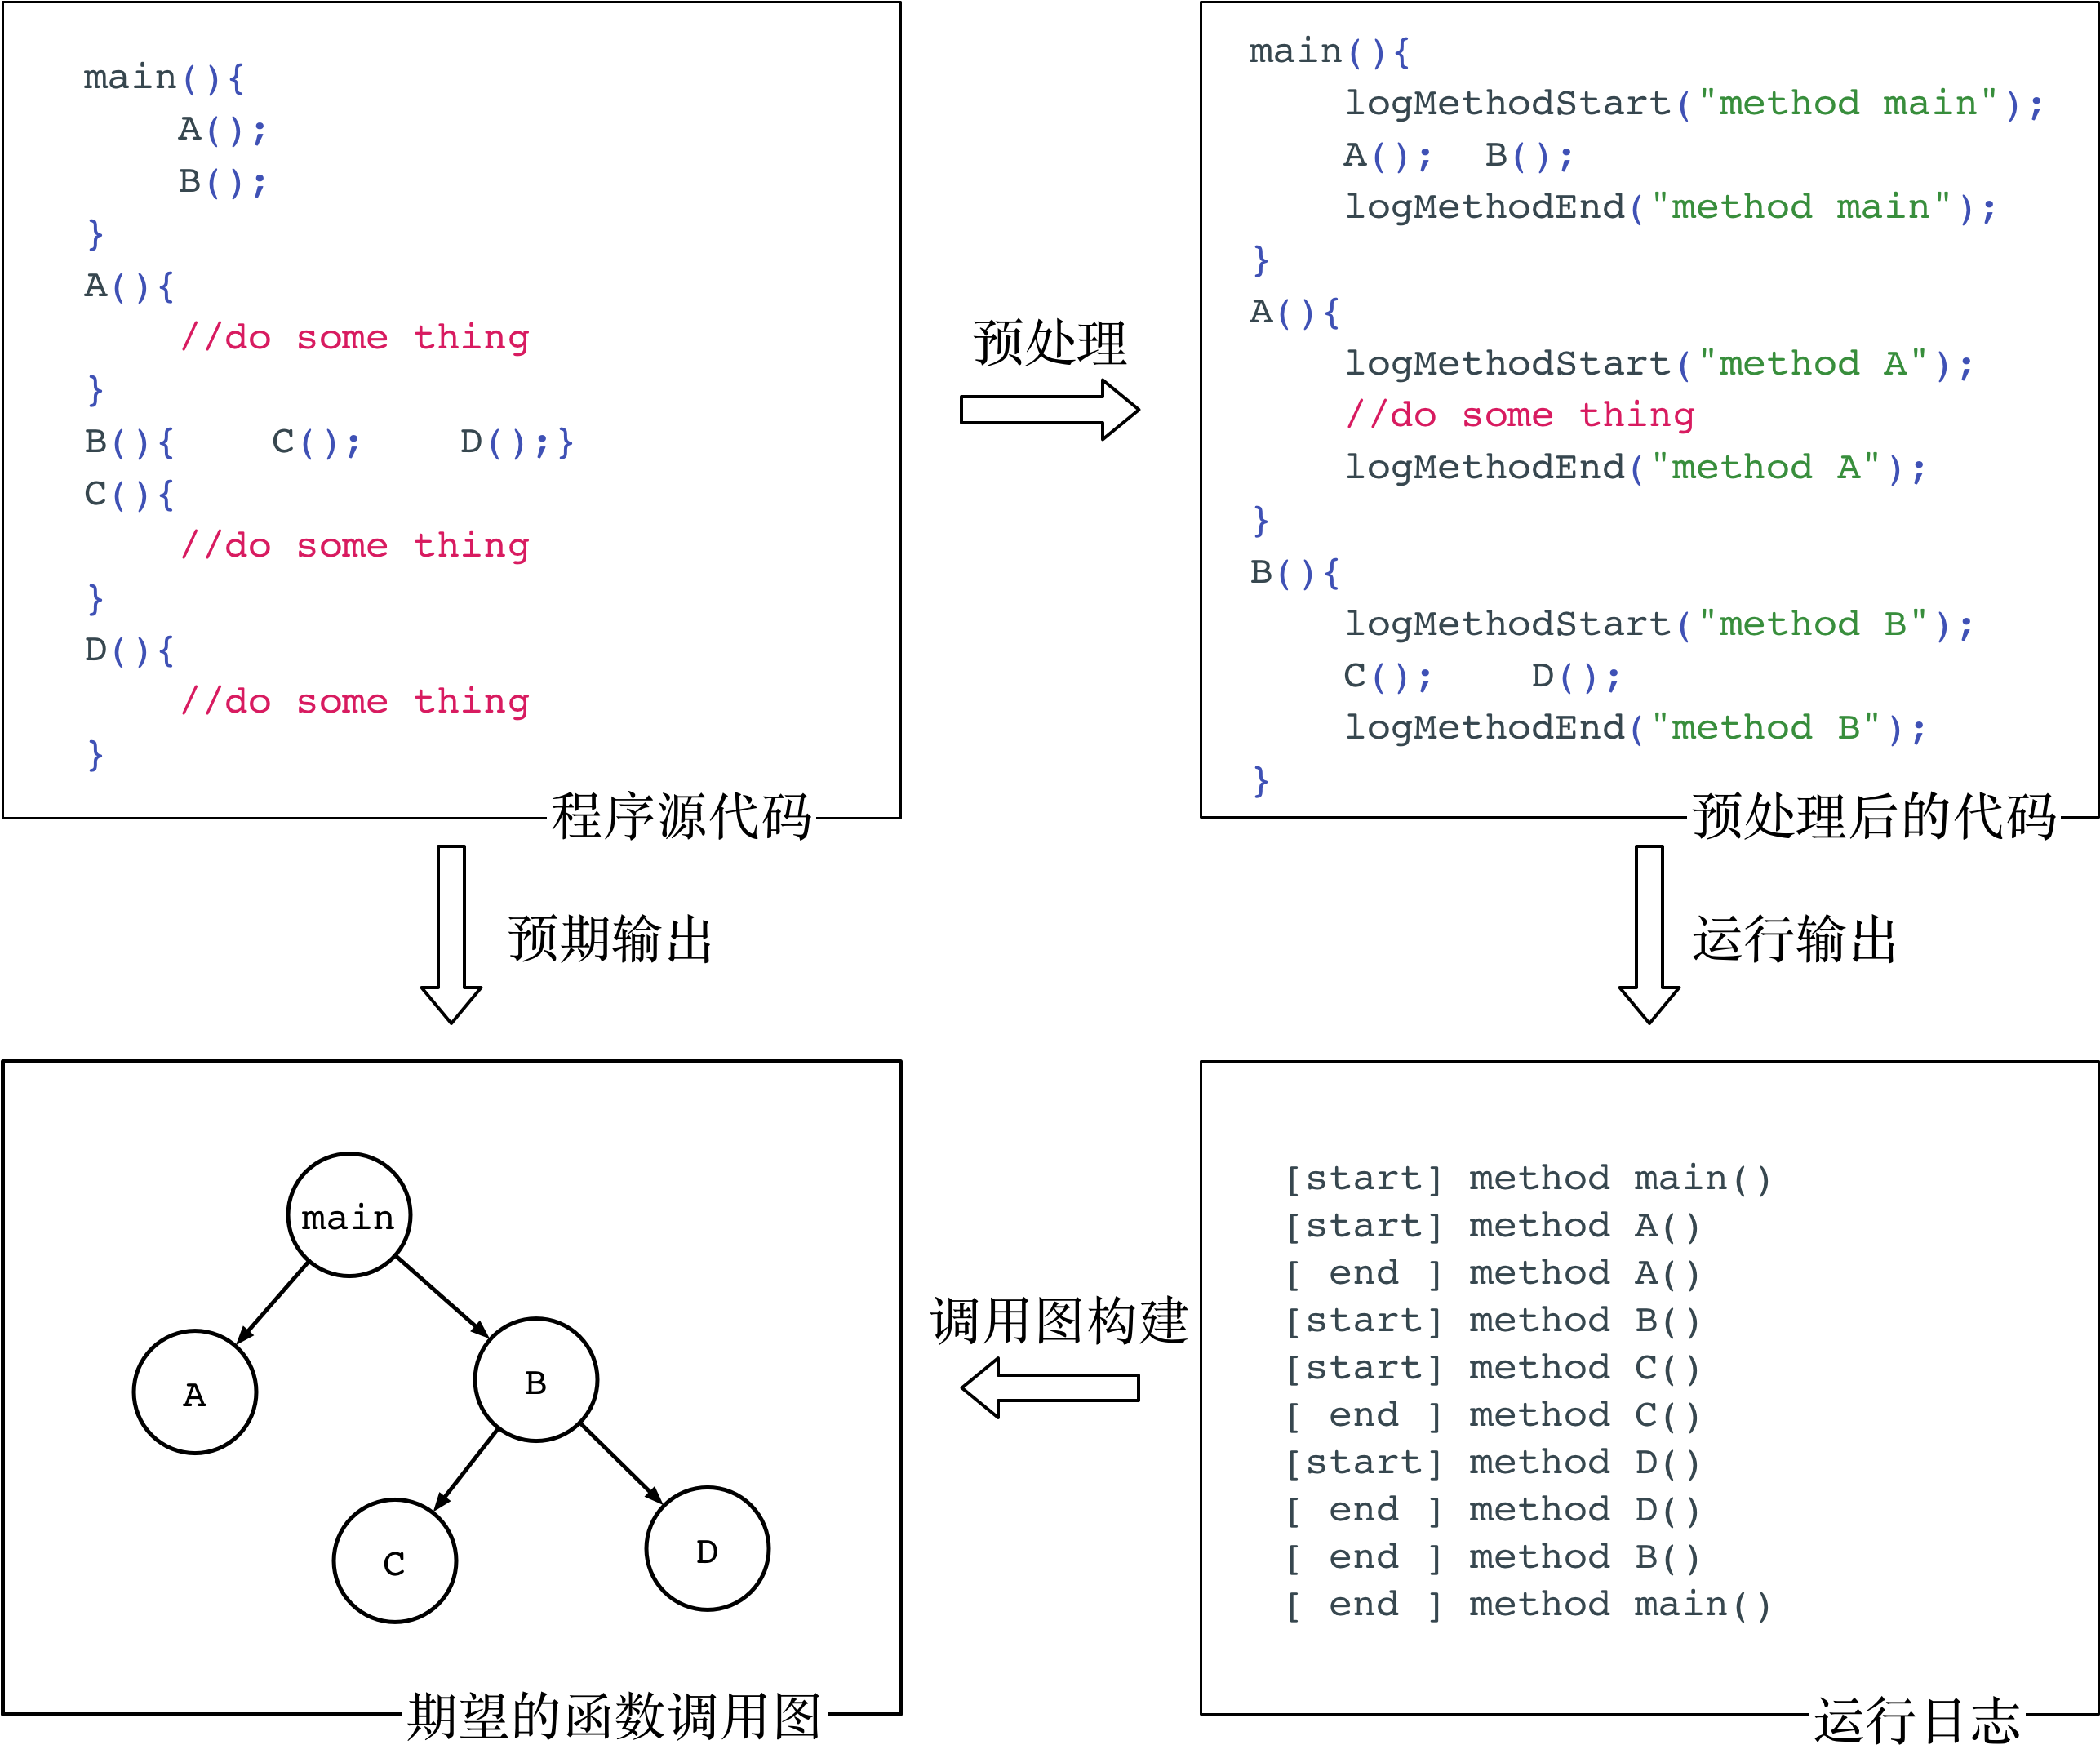
\includegraphics[width=0.8\textwidth]{./Figures/code-sample.png}
	\caption{RunDroid的处理流程}
	\label{fig:code_sample}
\end{figure*}


%在本节,
%以\autoref{fig:code_sample}为例,%简要介绍一下RunDroid还原Android应用程序的函数调用图的基本思路:
\autoref{fig:code_sample}-左上为一段示例代码:在main函数执行时,程序会依次调用A、B两个函数,而B函数则会调用了C、D两个函数。
\autoref{fig:code_sample}-左下则是程序的运行时函数调用图,即RunDroid实际的输出产物。
程序执行过程可以看做函数调用图的深度优先遍历过程。
还原函数调用图的关键点,在于如何在程序执行过程中输出树的遍历序列,并根据遍历序列进行还原函数调用图。
\eat{
通常的,树的遍历分为中序遍历、前序遍历以及后序遍历三种。
但是,两颗结构完全不同的树对应的遍历序列可能是一样的,
这也就意味着上述三种遍历方法均不能直接还原出函数调用图。
而且,函数执行过程中出现的错误异常可能使得序列输出中断,阻碍调用图的构建。
}
%本文采用的方案是利用在方法执行前后均记录执行日志(即一个方法的执行会输出两条日志:方法开始日志、方法结束日志),
%进行动态函数调用图的还原。

本文采用的技术方案:
RunDroid通过对源程序(\autoref{fig:code_sample}-左上)进行预处理,得到包含日志记录功能的运行代码(\autoref{fig:code_sample}-右上);
程序在函数执行前后可以输出和方法执行相关的日志信息,(\autoref{fig:code_sample}-右下);
最后,我们根据这些日志信息构建出函数调用图(\autoref{fig:code_sample}-左下)。
另外,在函数调用图的基础上,RunDroid利用日志中包括的方法对象信息,挖掘和方法对象相关联的方法,结合触发规则,进而建立方法触发关系,形成最终的\ecg。

% 从函数调用图的构建过程可以看出,程序的执行过程就是对函数调用图自上而下的深度优先遍历过程。由此可见,若要还原出图 6-右中的函数调用图,本文采用的基本思路是以日志方式输出对右图中的函数调用图的深度优先遍历序列,并基于得到的遍历序列还原出函数调用图。
% 由于Android是由面向对象编程语言Java开发的系统,系统还需要考虑面向对象编程的特性——多态性(即同一个行为在不同的对象下的表现可以不同)。为此,RunDroid还会在函数调用图将函数执行和对应的对象进行关联,更好地体现面向对象编程的函数调用关系。基于上述的函数调用关系的信息,RunDroid根据函数调用之间的关系进一步挖掘,进一步挖掘Android系统中的特性(例如组件Activity的生命周期、多线程的交互方式)。
%\section{总体框架}
\eat{


\begin{figure*}[!ht]
	\centering
	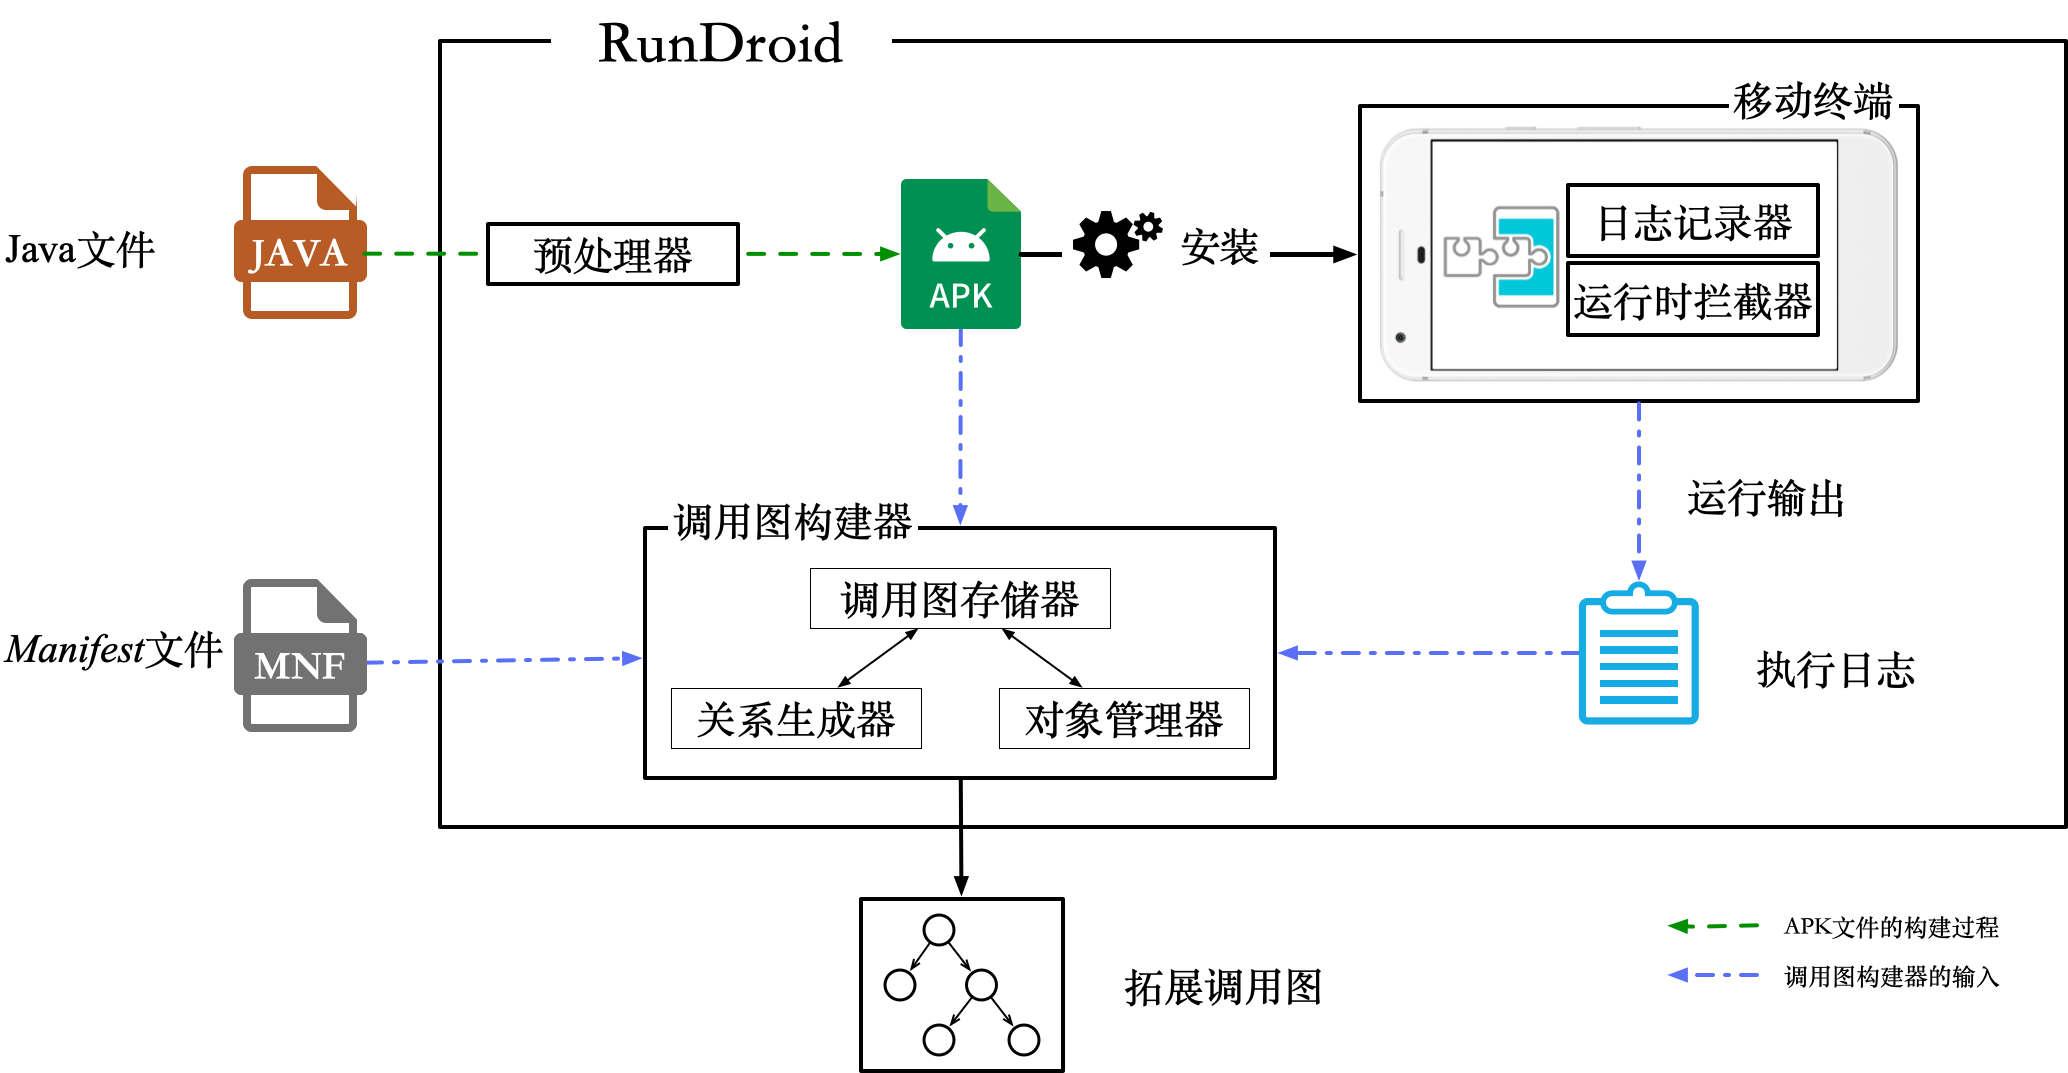
\includegraphics[width=0.8\textwidth]{./Figures/rundroid-overview.png}
	\caption{ RunDroid的工作流程}
%	\label{fig:rundroid_overview}
\end{figure*}

在技术实现上,RunDroid主要分为预处理器、运行时拦截器、日志记录器、调用图构建器等4个部分,对应的工作流程如\autoref{fig:rundroid_overview}所示。
从功能上,预处理器和运行时拦截器两者的作用是一致的:在程序运行过程中,当相关方法执行时,触发日志记录器记录相应的信息。
预处理器通过源代码插桩技术实现在用户方法运行时触发用户方法的信息记录,而运行时拦截器则是通过方法劫持技术实现对系统方法执行的拦截,进而触发日志记录。
%系统方法的执行。
%由于,用户方法层面的代码已修改,而系统方法的行为难以修改
%并非所有的方法都是进行日志代码织入的。RunDroid可以接触到用户方法(开发者在应用层面定义的方法)的源代码,而对于前者,
在应用运行时,日志记录器会以日志的形式将用户方法和系统方法对应的执行信息记录下来。
最后,调用图构建器会根据应用程序运行时输出的日志,构建拓展函数调用图。
}


%接下来,本章将从方法信息捕获和拓展调用图构建两个方面介绍RunDroid的设计。


% 本技术路线拟利用语法分析工具,对Android应用程序进行了应用源代码层面的执行日志插桩工作,利用非侵入式系统行为修改插件获取系统层面的函数执行信息。
% 结合以上日志信息,方案对日志进行初步处理,在图数据库上构建原始的Android应用程序的动态函数调用图。
% 通过阅读分析Android系统中多线程相关的源代码,制定具体的多线程分析插件,进而在函数调用图中标识出多线程相关的方法间触发关系,
%全面地展现Android应用的执行过程。


\section{方法信息的捕获}

在Android系统中,方法分为用户方法和系统方法两类。
用户方法是由用户定义的,直接修改的成本较低,易于修改其运行行为。
而系统方法在系统中定义,属于系统运行环境的一部份,行为修改成本较高。
虽然记录这两种方法的执行信息的方式是不一样的,但是两者最终的效果是一致的:当应用程序运行时,相关方法的执行信息均会以日志的形式记录下来,用于后续调用图的构建。


\subsection{用户方法执行信息的获取}%——基于源代码的日志代码插桩过程}

为了获取应用程序中用户方法的执行信息,RunDroid通过源代码插桩技术对应用做不影响业务逻辑的代码修改,产出包含日志代码的APK文件。
该APK在运行期间会以日志形式输出用户方法的执行信息。

%输出的APK文件在应用执行过程中将用户方法的执行信息输出出来。
RunDroid对用户方法进行源代码修改的处理过程如\autoref{alg:instrument}所示:
RunDroid会遍历项目源代码中的Java源文件,将源文件和对应的抽象语法树转化成XML格式的文件,并以DOM的形式加载到程序中(第3行)。
%  利用获取的语法结构,预处理器会提取出所有的方法体,
对于抽象语法树中的每一个类和每一个方法,RunDroid会计算出编译后所处的类的类名及方法签名(第4$\sim$\ref{alg:instrument:computeMethodId}行)。
全限类名和方法签名的组合<全限类名,方法签名>可以作为方法体的唯一标识,和抽象语法树中的方法体一一对应。
在每个方法内部,预处理器会插入用户方法日志记录的代码,实现日志代码编织,达到用户方法运行时信息记录的目的(第\ref{alg:instrument:addMethodExitLogCode}$\sim$\ref{alg:instrument:addMethodEnterLogCode}行)。
另外,预处理器还对每个方法体进行了异常捕获处理,防止方法体内部的异常导日志记录过程的中断,影响函数调用图的构建(第\ref{alg:instrument:addMethodCatchLogCode}行)。
上述操作都是对DOM对象\code{document}直接操作的。
当一个Java文件修改完毕后,预处理器会将DOM对象重新转换成Java源文件,并替换原来的文件(第\ref{alg:instrument:rewriteFile}行)。
最后,预处理器会利用编织后得到的源代码构建成APK文件(第\ref{alg:instrument:buildApk}行)。




\begin{algorithm}[!ht]
	\tablewuhao
	\caption{日志代码插桩过程} 
	\label{alg:instrument}
	\KwIn{ $javaFiles$,应用程序的源代码}
	\KwOut{ $apk$,包含插桩代码的APK文件}
	\SetKwProg{Fn}{Function}{:}{}
	
	\Fn{buildApk($log$)}{
		
		\For{$ javaFile \in javaFiles $}{
			

			将源文件 $javaFile $ 的抽象语法树转化成DOM对象 document;
						
			\For{ \emph { $ classEle \in document$}}{
				
				$className $ ~ $\gets  $ ~ computeClassName($classEle$,$xmlFile$); 	
				
				\For{\emph { $methodEle \in  classEle $}}{
					
					$methodId $ ~ $\gets $~ computeMethodId($methodEle$,$className$ ); 	 \label{alg:instrument:computeMethodId}
					
					addMethodExitLogCode($methodEle$,$methodId$);\label{alg:instrument:addMethodExitLogCode}
					
					addMethodCatchLogCode($methodEle$,$methodId$);  \label{alg:instrument:addMethodCatchLogCode}
					
					addMethodEnterLogCode($methodEle$,$methodId$);\label{alg:instrument:addMethodEnterLogCode}
				}
				
			}
		将  $document$ 转化成新的Java文件 $newJavaFile$; \label{alg:instrument:rewriteFile}
			
		}
		$	apk  \gets$ buildApk($newJavaFiles$)  \label{alg:instrument:buildApk}
		
		\KwRet{apk };
	}
	
\end{algorithm}
\subsection{系统方法执行信息的获取}%——基于动态拦截技术的方法信息捕获}


由于无法直接对系统方法进行源代码修改,RunDroid利用动态拦截技术对系统方法的执行进行拦截,达到获取系统方法的执行信息的目的。
RunDroid为待拦截的系统方法维护了一个系统方法列表,具体如\autoref{tbl:hookMethodList}所示。
列表中的方法通常和Android特性相关,涵盖Activity的生命周期方法、Java Thread API以及Handler机制等多个方面。


在目标应用程序开始运行前,RunDroid会为上述目标方法注册执行回调函数。
在目标方法执行前和执行后,对应的回调函数会被执行,进而通过日志记录器记录下这些方法执行的相关信息。
在RunDroid中,系统方法执行信息的获取,可以填补调用图缺失的系统方法执行,进而还原出应用层和系统层之间以及系统内部的方法调用,使得产生的调用图更加完整。

{
\begin{table*}[!ht]
	%	\centering
	\tablewuhao		
	
	\caption{待拦截的系统方法列表}
	
	\label{tbl:hookMethodList}
	
	
	\resizebox{\textwidth}{!}{
		\begin{threeparttable}[b]
			
			\begin{tabular}{|l|c|}
				\hline
				方法签名&说明\\
				\hline
				Activity.onCreate(Bundle)   &\multirow{6}{0.4\linewidth}{\centering 和Activity生命周期相关的方法}\\
				%	\cline{1-1}
				Activit.onStart()    &\\
				Activity.onResume()     &\\
				Activity.onPause()    &\\	
				Activity.onStop()     &\\
				Activity.onDestroy()    &\\
				\hline
				
				Thread.start()   & 和Java 线程启动相关的方法\\
				\hline
				Message.obtain() & \multirow{15}{0.4\linewidth}{\centering 和 Hanlder机制相关的方法}\\
				Handler.enqueueMessage(MessageQueue,Message,long)&\\
				Handler.dispatchMessage(Message)&\\
				Handler.post(Runnable)&\\
				Handler.postAtTime(Runnable,long)&\\
				Handler.postAtTime(Runnable,Object,long)&\\
				Handler.postDelayed(Runnable,long)&\\
				Handler.postAtFrontOfQueue(Runnable)&\\
				Handler.sendMessage(Message)&\\
				Handler.sendEmptyMessage(int)&\\
				Handler.sendEmptyMessageDelayed(int,long)&\\
				Handler.sendEmptyMessageAtTime(int,long)&\\
				Handler.sendMessageAtFrontOfQueue(Message)&\\
				Handler.sendMessageDelayed(Message,long)&\\
				Handler.sendMessageAtTime(Message,long)&\\
				
				\hline
				
				
				%		AsyncTask execute [Object& \multirow{3}{0.4\linewidth}{和 AsyncTask相关的方法}\\
				%		AsyncTask publishProgress [Object&\\
				%		AsyncTask executeOnExecutor Executor [Object &\\
				%		\hline
				
				
			\end{tabular}
			
			%		\begin{tablenote}
			%		\end{tablenote}
			
		\end{threeparttable}
	}
\end{table*}
}
\section{\ecg 的构建过程}

RunDroid构建拓展函数调用图的过程分为如下几个阶段:
根据程序运行时的日志提取函数间的调用关系,创建函数调用图;
根据AndroidManifest.xml的Activity组件声明,在函数调用图上标识出完整的Activity 生命周期流转序列;
利用方法执行与方法对象的关联关系,结合触发关系规则,补全方法间的触发关系,形成最终的拓展函数调用图。



\subsection{构建函数调用图}


\begin{algorithm}[!hb]
\tablewuhao
	\caption{函数调用图的构建过程} 
	\label{alg:buildCG}
	\KwIn{ $logs$,应用程序的运行时日志}
	\KwOut{ $ecg$, 拓展函数调用图}
	\SetKwProg{Fn}{Function}{:}{}
	
	\Fn{buildExtendedCallGraph($log$)}{
		
		$ecg$ $\gets$ new ExtendedCallGraph();
		
		\For{thread $\in$ $logs.threads$}{
			
			$stack$ $\gets$ new Stack();
			
			\For  {$log$ $\in$ $logs.get(thread)$}{
				
				$top$ = $stack$.peek() ;  
				
				\eIf{isMethodStartLog($log$)} {
					
					$m \gets $ generateMethodInfo($log$);
					
					$ecg$.addMethodNode($m$);
					%\Comment 在调用图中提交方法节点 
					
					$ecg$.addMethodObjectsIfNotExists($ o_p $,$o_i $) 	;							
					
					$ecg$.addMethodObjectRels($ \left\langle  o_p \joinrel\xrightarrow{parameter}   m \right\rangle   $,$ \left\langle  o_i \joinrel\xrightarrow{instance}   m \right\rangle  $) ;
					
					%	\Comment 在调用图中提交方法对象节点 (此处只涉及参数关系和实例关系)
					
					\If {  $top \neq null $ }{
						
						$ecg$.addInvokeRel($ \left\langle  top \to  m \right\rangle  $) ;
						
						$stack$.push($m$);
					}
					
				}{ 
					
					$ecg$.addMethodObjectIfNotExists($  o_r  $) ;
					
					$ecg$.addMethodObjectRel($ \left\langle   o_r \joinrel\xrightarrow{return}   m \right\rangle  $) ;
					
					%		  \Comment 在调用图中提交方法对象节点 (此处只涉及返回值关系)
					
					$stack$.pop() ;
					
				}
				
				
				
			}
		}
		\KwRet{ $ecg$};
	}
	
\end{algorithm}


%虽然所有线程的方法日志输入到同一个文件中,但是,从单个线程的视角看这些日志,日志在时间维度上的先后顺序就是对调用图的深度遍历。
%已检测的应用程序将日志输出到单个文件中。
%虽然所有线程的日志都输出到一个日志文件中,但在每个线程的视图中,日志条目的输出顺序遵循调用图的顺序遍历:调用方法在被调用方法之前输出。
%此外,每个方法执行对应于两个日志条目:方法入口和出口的日志条目。

由于在程序执行过程中,不存在一个调用关系跨越两个线程,因此,在整个构建过程中,RunDroid以产生日志的线程为基本构建单元,向调用图添加方法调用关系。
函数调用图的构建过程如\autoref{alg:buildCG}所示。

对于每个线程,RunDroid顺序遍历对应的日志,使用栈$stack$的入栈、出栈操作来模拟对应线程的函数执行的过程,还原调用关系(第2$\sim$ 20行):
当读取到方法执行的开始日志时,系统会在调用图创建一个节点表示该方法的执行(第7$\sim$8行),
同时也在调用图中添加方法参数、方法实例对应的对象节点$o_p$、$o_i$以及方法对象和方法的关系$ \left\langle  o_p \joinrel\xrightarrow{parameter}   m \right\rangle   $、$ \left\langle   o_i \joinrel\xrightarrow{instance}   m \right\rangle  $(第9$\sim$10行)。
如果此时当前线程栈$stack$的栈顶方法元素$top$存在,系统会创建从方法$top$到当前方法$m$的调用关系,$\left\langle top \to m \right \rangle  $,并将当前方法$m$压入栈$stack$中(第11$\sim$ 14行)。
当读取到方法执行的结束日志时,该日志对应的方法必然是栈顶方法$top$,若栈顶方法$top$存在返回对象$o_r$,则只需要将$o_r$和$top$的关系添加到调用图中即可,最后弹出栈顶的$top$即可(第 16$\sim$ 18行)。
在上述过程中,如果待添加的方法对象在调用图中已存在,该对象复用调用图原有的对象节点即可,无须重新添加,只需添加方法与对象间的关系即可。




% 当日志条目表示方法条目时,将根据日志条目和来自的4元组信息创建节点 日志存储在节点中(第6行)。
%然后,从堆栈顶部的方法到日志条目中的方法(第7-9行)构建调用关系。
%处理完调用关系后,该方法将被推入堆栈。当日志条目表示方法退出时,堆栈将弹出顶部的方法节点(第11-12行)。
%重复该过程,直到没有为一个线程留下日志条目,然后将为日志文件中的另一个线程启动相同的进程。

%构建扩展调用图。 
%DROIDSTITCHER通过添加表示已识别触发关系的边来扩展调用图。
%请注意,触发器关系中的目标方法通常是回调方法的调用图的入口点。
%因此,通过将触发关系添加为边,将所有调用图拼接成一个调用图作为输出。



\subsection{构建Activity的生命周期及事件回调的触发关系}

\point{构建Activity的生命周期}


Android 应用的Acticvity生命周期的构建就是将Activity生命周期方法按照时间顺序串联。%,利用的是\code{Activity}生命周期方法的签名的不变性。
生命周期的构建过程以AndroidManifest文件作为输入,在原有的函数调用图的基础上,添加Activity生命周期变化的有向边,具体过程如\autoref{alg:buildActivityLifecycle}所示:
对于AndroidManifest文件中声明的每一个Activity组件对象 $o_{activity}$,系统都会遍历以该对象为方法实例的方法$m$(即$m$、$o_{activity}$满足条件$o_{activity} \joinrel\xrightarrow{instance} m$);
若方法$m$同时满足三个条件,则将它添加到列表$lifecycleList$中(第7$\sim$11行)。
最后,将列表$lifecycleList$按照时间顺序进行排序,并依次连接起来,即可得到{Activity}的生命周期(第12$\sim$13行)。

这三个条件分别为:
(1)方法$m$的方法签名和\autoref{fig:Activity-lifecycle}中的任何一个生命周期方法的签名保持一致;
(2)方法$m$执行时所处的线程为主线程;
(3)方法$m$在调用图$cg$中不在调用者,即在调用图$cg$中不存在方法$m' \in cg$,使得$m' \to m $成立。

通常情况下,条件(1)$\sim$ (2)可以筛选出Activity组件相关的生命周期方法。
但是,当生命周期方法重写时,子类方法往往需要回调父类方法,执行系统在该状态下的业务逻辑。
例如,在重写方法\code{onCreate()}时,开发人员会调用\code{super.onCreate()}以完成Activity窗体的初始化。
若只考虑前面两个条件,两个方法均会被看作生命周期方法。
子类方法作为系统回调的一部分,应当保留在Activity的生命周期中,父类方法被子类方法调用,属于用户调用的范畴。
为了区分上述两类场景下的方法调用,我们需要在筛选生命周期方法时考虑条件(3)。



\begin{algorithm}[!hb]
\tablewuhao
	\caption{构建Activity的生命周期和事件回调} 
	\label{alg:buildActivityLifecycle}
	\KwIn{ $manifestFile$,AndroidManifest文件\\ \qquad  \quad $ecg$,函数调用图}	
	\KwOut{ $ecg$,包括Activity生命周期的函数调用图}
	
	
	
	\SetKwProg{Fn}{Function}{:}{}
	
		\Fn{patchActivityLifecycleAndUiEvent($ecg$)}{
		
		patchActivityLifecycle($ecg$,$manifestFile$);
		
		patchUiEvent($ecg$);

		\KwRet{$ecg$};
	}
	
	
	\Fn{patchActivityLifecycle($ecg$,$manifestFile$)}{
		
		
		$lifecycleList \gets$ new   $ List()$;
		
		
		\For{ \emph{ $o_{activity} \in \{ act \mid act $ 为文件 $manifestFile $中定义的Activity$ \} $ }}{
			
			
			
			\For{ \emph{ $m \in \{ m \mid  m$ 为调用图 $ ecg $中以$o_{activity}$为实例的方法节点$\}$}}{
				
				
				\If{ \emph{ $m$ 为Activity的生命周期方法  ~ \&\& ~   $m$ 的执行线程为主线程\\\qquad
						\&\&  $  \left\langle  m' \to m \right\rangle  \notin ecg$
				} }{
					
					$lifecycleList$.add($m$);
				}
				
				
			}
		}
		
		sortListByTime($lifecycleList$);
		
		linkItemsByTime($lifecycleList$,$ecg$);
		
	}
	% $o_p \stackrel{parameter}{\longrightarrow} m$
	\Fn{patchUiEvent($ecg$)} {
		\For{\emph{$o_{view} \in \{ o \mid o $ 为调用图 $ ecg $中{View}类型的对象节点  $ \}$} }{ 
			\For{\emph{$o_{listener} \in \{ o \mid o $  为调用图 $ ecg $  中{View.OnClickListener} 类型的对象节点 $ \}$} }{		
				\If {\emph{$o_{view}$,$o_{listener}$,$m_{register}$ 和 $m_{click}$  满足\autoref{equ:rule_ui}}
					}{
					$ecg$.addTriggerRel($m_{register} \lhook\joinrel\xrightarrow{UiEvent}  m_{click} $)	
				}
			}
		}
	}		
\end{algorithm}


\point{构建Andoid事件回调的触发关系}

在构建Andoid事件回调的触发关系时,我们会遍历拓展调用图中的所有{View}类型的对象节点$o_{view}$和{View.OnClickListener}类型的对象节点$o_{listener}$的组合。
对于组合$\left\langle o_{listener}  , o_{view}\right\rangle $,若调用图中存在方法节点$m_{register} $、$m_{click} $满足\autoref{equ:rule_ui},方法节点$m_{register} $、$m_{click} $之间添加从$m_{register} $指向$m_{click} $的有向边,即$m_{register} \lhook\joinrel\xrightarrow{UiEvent}  m_{click}  $(第15$\sim$18行)。


%Andoid事件回调的触发关系描述的是控件点击事件的注册和响应之间的因果关系,即方法\code{View.setOnClickeListener(View\$OnClickListener)}(用$m_{register}$表示)和\code{View\$OnClickListener.onClick(View)}间的因果关系(用$m_{click}$表示)。
%根据第\ref{chp:definition}章中方法触发关系的相关定义,$m_{register} \lhook\joinrel\xrightarrow{UiEvent}  m_{click}  $ 成立。
%我们观察发现:方法$m_{register}$的实例对象$o_{view}$是方法$m_{click}$的参数对象,而方法$m_{register}$的参数对象$o_{listener}$是方法$m_{click}$的实例对象。
%因此,在构建Andoid事件回调的触发关系过程中,当方法$m_{register} $、$m_{click} $满足第19$\sim$22行的条件时,这两个方法之间存在触发关系,即$m_{register} \lhook\joinrel\xrightarrow{UiEvent}  m_{click}  $(第23行)。


\eat{
基于Java的多线程交互往往是以\code{Runnable}作为传递对象,通常通过调用方法\code{Thread.start()} (用$m_{start}$表示)和\code{Activity.runOnUiThread(Runnable)}(用$m_{runOnUiThread}$表示)等API,进而触发方法\code{Runnable.run()}(用$m_{run}$表示)的执行。
因此,对于方法\code{Thread.start()},如果存在一个\code{Runnable}类型的对象\code{r},它既是方法$m_{start}$的实例,又是方法$m_{run}$的实例,则两个方法间存在触发关系,即$m_{start} \hookrightarrow m_{run}$(第8 $\sim$10行)。
同样的,对于方法\code{Activity.runOnUiThread(Runnable)},也存在类似的关系:
如果存在一个\code{Runnable}类型的对象\code{r},它既是方法$m_{runOnUiThread}$的参数,又是方法$m_{run}$的实例,则两个方法间存在触发关系,即$m_{runOnUiThread} \hookrightarrow m_{run}$(第11 $\sim$13行)。
}


 \subsection{构建多线程触发关系}
基于函数调用图构建多线程触发关系主要分为两个方面,基于Java 的多线程交互与基于{Handler} 的多线程消息调度,具体的过程如\autoref{alg:buildTrigger}所示。



\begin{algorithm}[!ht]
	\tablewuhao
	\caption{扩展函数调用图的构建过程}
	\label{alg:buildTrigger}
	\KwIn {	$ecg$, 拓展函数调用图} 
	\KwOut {	$ecg$,包含触发关系的拓展函数调用图}
	
	
	\SetKwProg{Fn}{Function}{:}{}
	\Fn{addTriggerRels($ecg$)}{
	
		{// 在调用图$ecg$中创建基于Java 多线程交互的触发关系}
		
		
		\For{\emph{$o_{thread} \in \{ o \mid o $  为调用图$ecg$中的 {Thread} 类型的对象节点 $ \}$} }{
			\If{ \emph{$o_{thread}$、$m_{start}$ 和 $m_{run}$  满足\autoref{equ:rule_thread}}}{
				$ecg$.addTriggerRel($m_{start} \lhook\joinrel\xrightarrow{Thread}  m_{run} $)	
			}}
		\For{\emph{$o_r \in \{ o \mid o $  为调用图$ecg$中的  {Runnable} 类型的对象节点$  \}$} }{
			\If{ \emph{$o_r$、$m_{runOnUiThread}$ 和 $m_{run}$  满足\autoref{equ:rule_runOnUiThread}}}{
				$ecg$.addTriggerRel($m_{runOnUiThread}  \lhook\joinrel\xrightarrow{runOnUiThread}  m_{run} $)	
			}	
		}
		{// 在调用图$ecg$中创建基于{Handler} 多线程消息调度的触发关系}
		
		
			\For{\emph{ $o_m \in  \{ o\mid  o $  为调用图$ecg$中的 {Message} 类型的对象节点$\}$} }{
			\If{ \emph{$o_m$、$m_{handle}$和 $m_{dispatch}$  满足\autoref{equ:rule_handler}}}{
		%		\tcp{Here means $m_{enqueue} \lhook\joinrel\xrightarrow{Handler} m_{dispatch} $.}
			
				$m_{send}  \gets $   calculateSendMethod($ecg$,$m_{enqueue}$);
				
				$m_{handle} \gets$  calculateHandleMethod($ecg$,$m_{dispatch}$);
				
				$ecg$.addTriggerRel($m_{send} \lhook\joinrel\xrightarrow{Handler} m_{handle} $ )	
			}	
		}
		\KwRet $ecg$;
	}
	
\end{algorithm}


\point{基于Java 的多线程交互}


基于Java的多线程交互往往是以{Runnable}作为传递对象,通常通过调用方法\code{Thread.start()} 和\code{Activity.runOnUiThread(Runnable)}等API,进而触发类{Thread}和{Runnable}的方法\code{run()}的执行。

对于方法\code{Thread.start()} 相关的触发关系,我们会遍历拓展调用图中的所有{Thread}类型的对象节点$o_{thread}$。
判断调用图中是否存在方法节点$m_{start} $、$m_{run} $以及对象节点$o_{thread}$满足\autoref{equ:rule_thread},方法节点$m_{start} $、$m_{run} $之间添加从$m_{start} $指向$m_{run} $的有向边,即$m_{start} \lhook\joinrel\xrightarrow{Thread}  m_{run}  $(第2$\sim$4行)。


对于方法\code{Activity.runOnUiThread(Runnable)}相关的触发关系,我们会遍历拓展调用图中的所有{Runnable}类型的对象节点$o_{r}$。
判断调用图中是否存在方法节点$m_{runOnUiThread} $、$m_{run} $以及对象节点$o_{r}$满足\autoref{equ:rule_runOnUiThread},方法节点$m_{runOnUiThread} $、$m_{run} $之间添加从$m_{runOnUiThread} $指向$m_{run} $的有向边,即$m_{runOnUiThread} \lhook\joinrel\xrightarrow{runOnUiThread}  m_{run}  $(第5$\sim$7行)。


%基于Java的多线程交互往往是以\code{Runnable}作为传递对象,通常通过调用方法\code{Thread.start()}和\code{Activity.runOnUiThread(Runnable)}等API,进而触发方法\code{Runnable.run()}(用$m_{run}$表示)的执行。
%因此,对于方法\code{Thread.start()},如果存在一个\code{Runnable}类型的对象\code{r},它既是方法$m_{start}$的实例,又是方法$m_{run}$的实例,则两个方法间存在触发关系,即$m_{start} \hookrightarrow m_{run}$(第8 $\sim$10行)。
%同样的,对于方法\code{Activity.runOnUiThread(Runnable)},也存在类似的关系:
%如果存在一个\code{Runnable}类型的对象\code{r},它既是方法$m_{runOnUiThread}$的参数,又是方法$m_{run}$的实例,则两个方法间存在触发关系,即$m_{runOnUiThread} \hookrightarrow m_{run}$(第11 $\sim$13行)。

%在构建基于Java 多线程交互的触发关系时,


%我们会遍历拓展调用图中的所有\code{View}类型的对象节点$o_{view}$和\code{View.OnClickListener}类型的对象节点$o_{listener}$的组合。
%对于组合$<o_{listener}$,$o_{view}>$,若调用图中存在方法节点$m_{register} $、$m_{click} $满足\autoref{equ:rule_ui},方法节点$m_{register} $、$m_{click} $之间添加从$m_{register} $指向$m_{click} $的有向边,即$m_{register} \lhook\joinrel\xrightarrow{UiEvent}  m_{click}  $(第16$\sim$19行)。




\eat{\begin{equation}
	\label{equ:rule_1}
	\left. \begin{gathered}
	o_r    \        is           \      Runnable  \      Class \\
	rel(m_{start}, o_r) = instance \\
	rel(m_{run}, o_r) = instance \\
	\end{gathered} \right\}
	\Rightarrow  m_{start} \hookrightarrow m_{run}. 
	\end{equation}
}



\eat{
\begin{equation}
\label{equ:rule_2}
\left. \begin{gathered}
o_r    \        is           \      Runnable  \      Class \\
rel(m_{runOnUiThread}, o_r) = parameter \\
rel(m_{run}, o_r) = instance \\
\end{gathered} \right\}
\Rightarrow  m_{runOnUiThread} \hookrightarrow m_{run}. 
\end{equation}
}








\point{基于{Handler} 的多线程消息调度}

根据第\ref{chp:background}、\ref{chp:definition}章的介绍可知,用户通过调用Handler提供的API,
将相关业务逻辑借助Message对象传递给目标线程的Handler对象,在目标线程执行相应的业务逻辑处理。
%在这个部分,我们需要找出用户调用的Handler API和对应目标线程的业务逻辑方法间的触发关系:
在构建{Handler} 触发关系过程中,首先,我们利用类{Handler}的方法\code{enqueueMessage(Message)}(用$m_{enqueue}$表示)和\code{dispatchMessage(Message)}(用$m_{dispatch}$表示)公用同一个Message对象的特点,
找到所有的Handler底层函数触发关系 ,$m_{enqueue}  \hookrightarrow  m_{dispatch}$ (第$8\sim$9 行);
对于每一个触发关系 $m_{enqueue}  \hookrightarrow  m_{dispatch}$,
从$m_{enqueue}$ 顺着调用关系往上找到最上层的Handler API方法(即用户调用的Handler API方法,$m_{send}$)(第10行),
从$m_{dispatch}$ 顺着调用关系往下找到用户定义的方法\code{Handler.handleMessage(Message)}$m_{handle}$(第11行),
最后在调用图中提交方法$m_{send}$和$m_{handle}$之间的触发关系 $m_{send} \lhook\joinrel\xrightarrow{Handler} m_{handle}$(第12行)。
%如果$m_{send}$和$m_{handle}$中有一个方法未找到,表示
最终,我们得到用户通过Handler进行多线程消息调度的用户层面方法的触发关系。


\eat{
MATCH (SEND:METHOD)-[:PARAM]->(MSG:OBJECT),

(SEND:METHOD)-[:INSTANCE]->(HANDLER:OBJECT),

(HANDLE:METHOD)-[:PARAM]->(MSG:OBJECT),

(HANDLE:METHOD)-[:INSTANCE]->(HANDLER:OBJECT)

WHERE SEND.methodSign ='boolean android.os.Handler.enqueueMessage(android.os.MessageQueue,android.os.Message,long)'

AND HANDLE.methodSign ='void android.os.Handler.dispatchMessage(android.os.Message)'

RETURN SEND,HANDLE
	
	
	
	
MATCH p=(method:METHOD)-[:INVOKE*0..]->(enqueue:METHOD),

(enqueue)-[:TRIGGER\_PREPARE\_HANDLER]->(dispatch:METHOD)

AND  NOT (enqueue)-[:INVOKE]->()

RETURN p,method,enqueue,dispatch;

	
	
MATCH p=(method:METHOD)-[:INVOKE*0..]->(enqueue:METHOD),

(enqueue)-[:TRIGGER\_PREPARE\_HANDLER]->(dispatch:METHOD)-[r:INVOKE]->(run:METHOD)

WHERE method.methodSign IN [

'boolean android.os.Handler.post(java.lang.Runnable)',

'boolean android.os.Handler.postAtTime(java.lang.Runnable,long)',

'boolean android.os.Handler.postAtTime(java.lang.Runnable,java.lang.Object,long)',

'boolean android.os.Handler.postDelayed(java.lang.Runnable,long)']

RETURN p,method,enqueue,dispatch, run

	
	
	
MATCH p=(method:METHOD)-[:INVOKE*0..]->(enqueue:METHOD),

(enqueue)-[:TRIGGER\_PREPARE\_HANDLER]->(dispatch:METHOD)

AND  NOT (enqueue)-[:INVOKE]->()

RETURN p,method,enqueue,dispatch

	

}

\eat{识别触发关系。
触发关系表示由于Android框架的生命周期事件,系统事件和多线程通信而导致的方法的隐式调用。
以Handler为例。 sendMessage方法隐式意味着稍后将执行相应的方法handlerMessage。
为了捕获这种关系,我们确定了一种模式:sendMessage方法通过传递消息对象来触发方法handlerMessage。
因此,如果我们可以找到用作方法sendMessage和方法handlerMessage的参数的消息对象,那么我们可以在这两个方法之间创建触发器关系。
在分析了Android框架的源代码之后,我们确定了线程,窗口小部件的侦听器注册和异步任务的类似模式。
因此,DROIDSTITCHER维护一个方法列表,这些方法是触发器关系的潜在目标,并比较这些方法中消息对象的内存地址以推断关系。
}



 \section{本章总结}

本章详细介绍了RunDroid的设计。
首先,本章简要说明了RunDroid实现的基本功能,然后具体解释说明RunDroid的整体运行流程。
在此基础上,本章介绍了RunDroid各个的流程的设计细节。
RunDroid利用源代码修改和运行时方法拦截相结合的方式,捕获用户方法和系统方法的执行信息,并以日志的形式保存方法执行信息。
RunDroid遍历各线程的方法执行日志结合栈的入栈、出栈操作,模拟各个线程的函数执行的过程,通过线程内部各个方法日志的嵌套关系还原出函数调用图,并在此基础上构建Activity的生命周期,补全方法间的触发关系,构建最终的拓展函数调用图。

\clearPaperPage



\chapter{RunDroid的系统实现 }

\label{chp:implement}

RunDroid使用Java作为开发语言,使用了srcML、Xposed、Neo4j等技术,由预处理器、运行时拦截器、日志记录器、调用图构建器等部分组成,整体架构图如\autoref{fig:rundroid_overview}所示。
%从功能上,预处理器和运行时拦截器两者的作用是一致的:在程序运行过程中,当相关方法执行时,触发日志记录器记录相应的信息。
预处理器通过源代码插桩技术实现在用户方法运行时触发用户方法的信息记录,而运行时拦截器则是通过方法劫持技术实现对系统方法执行的拦截,进而触发日志记录。
%系统方法的执行。
%由于,用户方法层面的代码已修改,而系统方法的行为难以修改
%并非所有的方法都是进行日志代码织入的。RunDroid可以接触到用户方法(开发者在应用层面定义的方法)的源代码,而对于前者,
在应用运行时,日志记录器会以日志的形式将用户方法和系统方法对应的执行信息记录下来。
最后,调用图构建器会根据应用程序运行时输出的日志,构建拓展函数调用图。

\begin{figure*}[!hb]
	\centering
	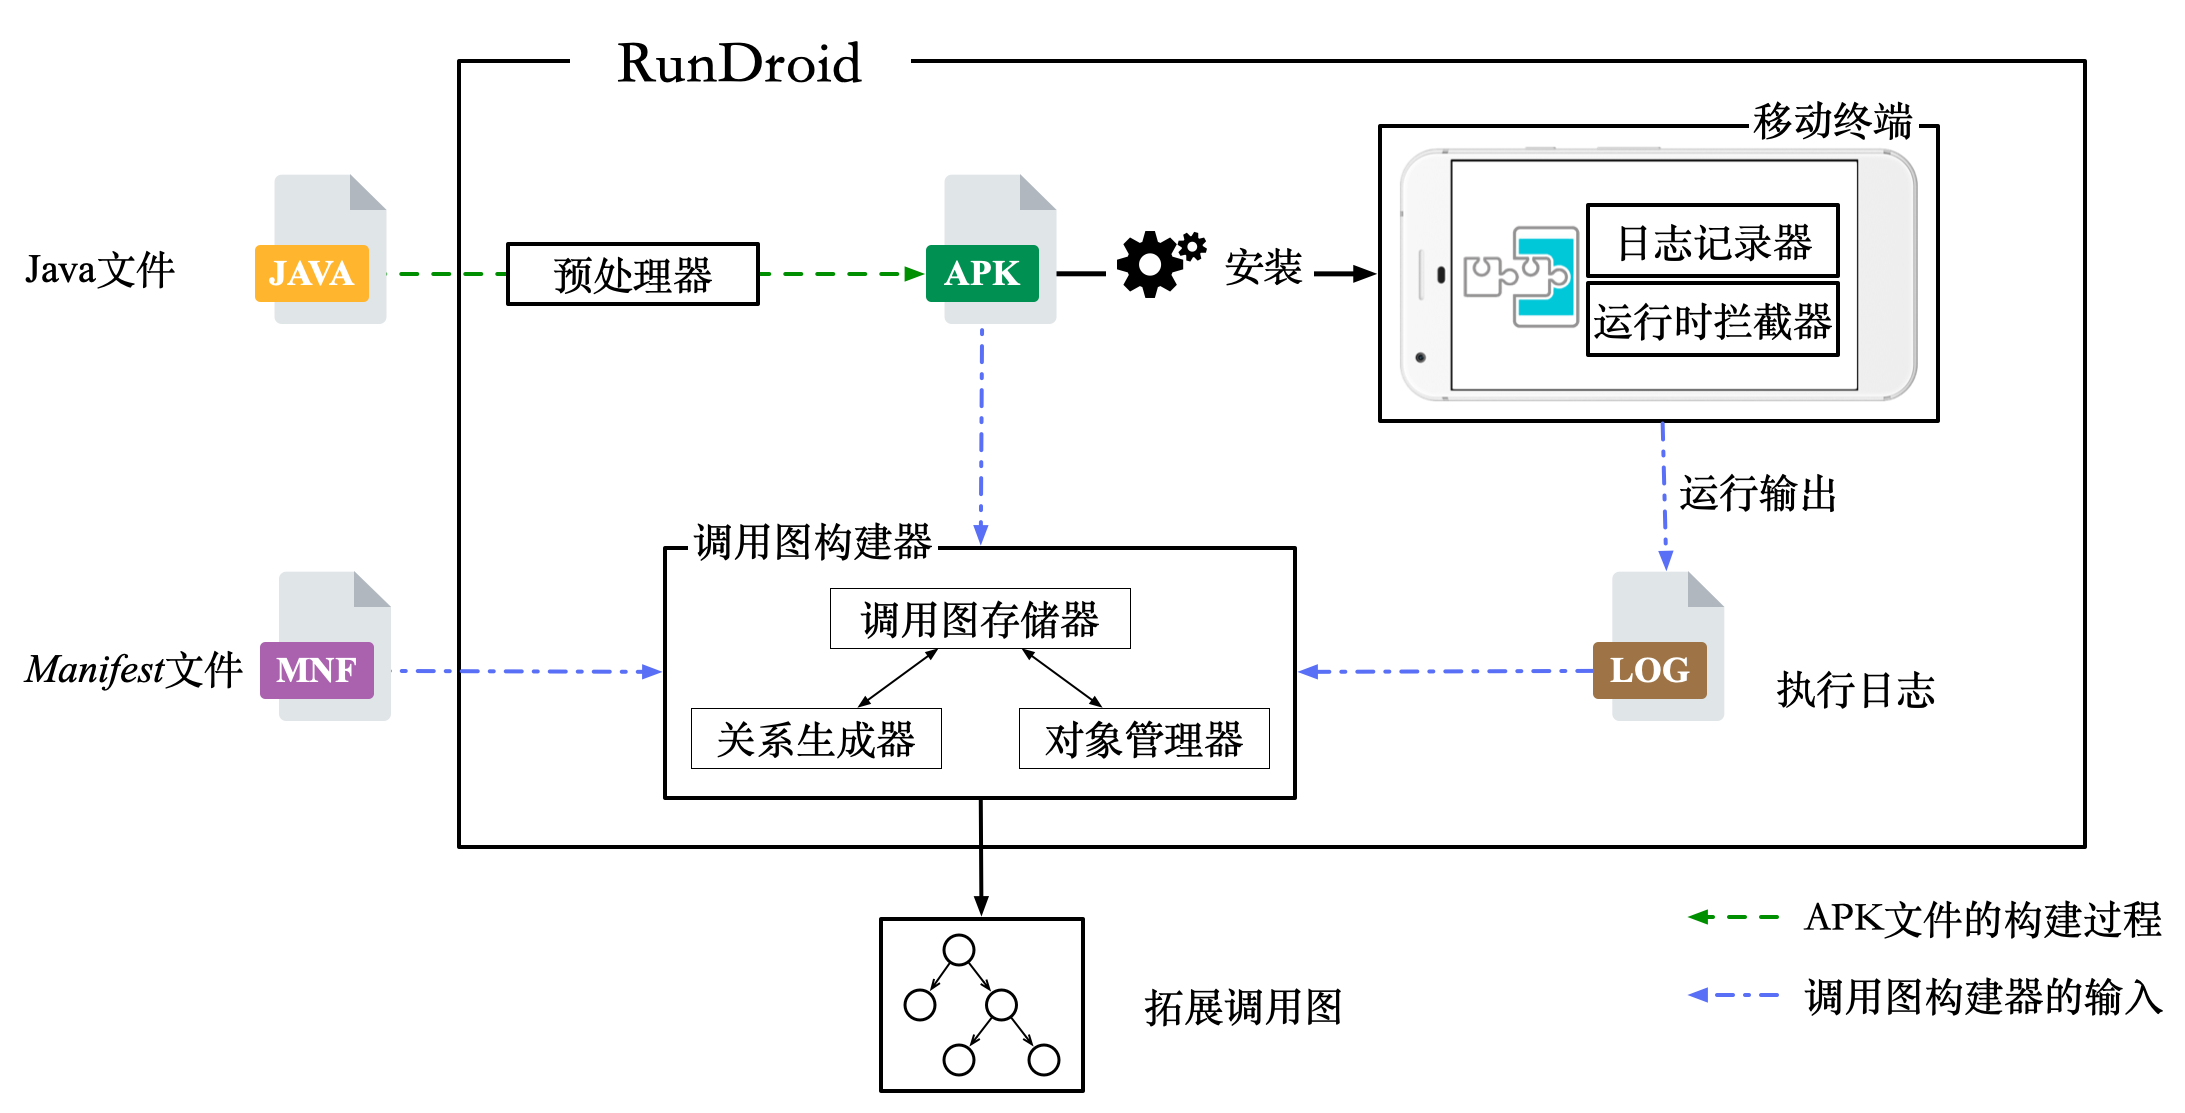
\includegraphics[width=0.8\textwidth]{./Figures/overview.png}
	\caption{ RunDroid的整体架构图}
	\label{fig:rundroid_overview}
\end{figure*}


\section{模块实现}



\subsection{预处理器}

预处理器在RunDroid中的作用主要是用户方法的日志代码编织。
在现有的技术上,代码编织主要分为两类:基于源代码的代码编织和基于字节码的代码编织。
字节码编织技术以技术成熟、应用广泛的AspectJ\cite{TheAspecJ} 为代表技术,。
但是,字节码插桩技术在运行过程中会生成过多的方法数,在Android应用构建过程中可能存在方法数65K限制问题。
为此,预处理器采用的方案是基于源代码的代码编织方案。

在实现上,预处理器利用轻量级源代码分析工具srcML\cite{collard2013srcml}对程序的源代码进行语法解析,将程序的抽象语法树转化成XML文件。
在XML文件的基础上,预处理器直接对每个方法体进行修改,实现日志代码的编织,最后重新转换成源代码,经过构建得到可以运行的APK文件。
该方案通过直接修改源程序,将日志记录代码写入在方法体内部,避免了新方法的引入,规避了方法数65K限制问题。

%它可以,支持C、C++、C\#以及Java等多个语言的语法解析。
%	同时,srcML还提供了一个强大工具集,支持对生成内容的查询、分析以及修改,可以用于架构设计、语言研究、软件重构等场景,应用于软件工程、编程语言、并行和分布式处理等多个领域。
%在RunDroid,srcML作为RunDroid预处理器中的重要组成部分,承担源代码语法解析的主要职责,辅助完成用户方法层面的日志代码的编织。
% 拦截器组件基于Xposed框架[5],它拦截在应用程序层和Android框架之间传递的消息。
% 拦截器记录在两个层之间进行的每个方法调用,并将它们与应用程序层中对应的方法调用相关联,以产生完整的方法调用跟踪。
% RunDroid维护感兴趣的方法列表,如生命周期方法和隐式回调,以便日志文件包含每次执行期间调用的方法调用

\subsection{运行时拦截器}%——系统方法的捕获}

%由于预处理器可以处理的方法需要
由于无法对系统方法的源代码进行直接修改,因此预处理器无法实现对系统方法的日志代码编织,无法达到系统方法信息记录的目的。
为了弥补预处理器的不足,RunDroid中的运行时拦截器需要在系统层面上实现对系统方法的拦截,实现后续方法信息的日志记录。


%Interceptor组件构建在Xposed框架[5]之上,它拦截在应用程序层和Android框架之间传递的消息。 
%Interceptor记录在两个层之间进行的每个方法调用,并将它们与应用程序层中的相应方法调用相关联,以生成完整的方法调用跟踪。
 %RunDroid维护一组感兴趣的方法,例如生命周期方法和隐式回调,以便日志文件包含每次执行期间调用的方法调用。

%xposed是一个模块框架,可以在不接触任何APKs的情况下改变系统和应用程序的行为。这很棒,因为这意味着模块可以在不做任何改变的情况下为不同版本甚至是rom工作(只要原始代码没有太多改变)。撤销也很容易。由于所有更改都在内存中完成,您只需关闭模块并重新启动即可恢复原始系统。还有许多其他优点,但这里还有一个:多个模块可以对系统或应用程序的同一部分进行更改。有了改进的APKs,你可以选择一个。除非作者用不同的组合构建多个APKs,否则无法将它们组合起来。


%posed是一个基于Android系统的运行时行为修改框架。
%在不修改程序源代码的情况下,基于Xposed开发的第三方插件通过将目标方法关联到函数执行回调上,进行方法参数和返回值的重写和额外方法逻辑的添加等操作,达到目标方法行为修改的目的。
%	Xposed的实现原理具体如下:由于Android系统的所有的应用程序进程都是由Zygote进程孵化而来,Xposed通过替换程序\code{/system/bin/app\_process},使得系统在启动程中加载Xposed的相关文件,将所有的目标方法指向Native方法xposedCallHandler,维护目标方法和对应的钩子方法(Hook Function)的映射关系,从而实现对Zygote进程及Dalvik虚拟机的劫持;
% 当程序执行到目标方法时,xposedCallHandler会完成目标方法的原有代码和对应钩子方法的调度,达到对目标方法劫持的目的。
%利用Xposed提供的类似面向切面编程的API接口,RunDroid中的运行时拦截器可以对任意方法(包括用户方法和系统方法)执行过程进行动态拦截,达到系统方法信息的日志记录的目的。


在实现上,运行时拦截器是基于Xposed\cite{Xposed}实现的插件,它维护的列表包括了所有需要拦截的系统方法。%,如\autoref{tbl:hookMethodList} 所示。
每当目标应用程序启动时,运行时拦截器通过Xposed提供的API\code{ XposedHelpers.findAndHookMethod()}将\autoref{tbl:hookMethodList}中的目标方法绑定到方法钩子(即\eat{Xposed提供的XC\_MethodHook的子类 ,}类HookCallBack)上。
在应用程序的运行过程中,HookCallBack对象的方法\code{beforeHookedMethod(MethodHookParam)}会在目标方法执行之前被调用,
方法\code{afterHookedMethod(MethodHookParam)}会在目标方法执行后调用。
上述两个方法的参数\code{MethodHookParam}中会包括该方法执行时的相关方法对象。
最终,HookCallBack对应会将方法执行的相关信息传递给日志记录器。



相比定制化Android系统,通过Xposed实现的运行时拦截器兼容性良好,适用于当前主流的Android系统版本,实现成本低。
同时,待拦截方法列表的编辑功能的引入,使得在不修改插件代码的情况下,支持动态添加删除待拦截的方法,避免了Xposed插件修改后的系统重启操作,提高了RunDroid整体的执行效率。
 

\subsection{日志记录器}

日志记录器的职责是将方法执行的消息以日志文件的形式进行持久化存储。
针对不同的方法类型(静态方法与非静态方法、用户方法与系统方法等),日志记录器提供了不同的API,帮助我们记录相应方法执行的日志信息。
在日志内容上,日志记录器还会记录每个方法执行的时间戳、所处线程、方法签名标识、所处阶段(方法开始执行阶段/方法执行完毕阶段)以及相关的方法对象信息。
方法对象信息主要包括对象的类型、属性和全局ID(通过Java API  \code{System.identityHashCode(Object)}获取)等。
同时,日志记录器还支持对象信息的自定义:开发人员可以根据自身的需要为不同类型的对象输出不同对象数据信息。
% 在底层实现上,考虑日志读入文件对程序执行效率的影响,我们评估了多种日志写入方式,最终我们发现基于mmap的日志记录方式效率最高,对程序运行的影响最小。




\subsection{调用图构建器}

% 调用图构建器的功能是拓展函数调用图的构建、存储和展现。
调用图构建器由调用图存储器、对象管理器和关系生成器组成,如\autoref{fig:rundroid_overview}所示。

调用图存储器将Neo4j\cite{Neo4jthe19}作为调用图的存储引擎,承担着拓展函数调用图的存储、查询、展示的职责。
Neo4j的数据分为节点和关系两种类型,支持自定义键值属性。
同时,Neo4j可为节点指定标签,为关系指定类型,用于区分不同含义的节点和关系。
拓展函数调用图中的数据在Neo4j中的表现形式如下:
调用图中的方法和对象会以节点的形式出现在调用图中, 方法节点的标签分为\code{METHOD}和\code{FRAMEWORK},对象节点的标签为\code{OBJECT};
方法间关系分为调用关系和触发关系,分别用关系\code{INVOKE}和\code{TRIGGER}表示;
方法和对象之间的关系分为参数关系、返回值关系和实例关系,分别用关系\code{PARAMETER}、\code{RETURN}、\code{INSTANCE}表示。




\eat{
	Neo4j是基于Java语言开发的图数据库,可以用于存储图结构相关的数据结构。
	%与传统的基于关系模型的存储结构不同,Neo4j的存储模型是基于图论开发的,遵循属性图数据模型。


	在数据操作接口方面,Neo4j支持Cypher、Java API和RESTful API等方式,提供友好的数据浏览界面用于数据的展示与修改。
	\eat{由于基于属性图数据模型,Neo4j通常适用于和图关系有着密切关系的应用场景:例如社交网络分析,公共交通网络研究以及地图网络拓扑等场景。}
	在RunDroid,Neo4j是调用图构建器的主要组成部分,承担着拓展函数调用图的存储、查询、展示的职责。
}


对象管理器负责将日志中的对象信息映射成调用图中的节点。
通常情况下,我们认为对象和全局ID一一对应,所以,我们将全局ID相同的对象信息映射成调用图中的一个节点。
但考虑到有些类型(例如Handler机制中的Message)使用对象池技术,我们还在全局ID的基础上引入对象版本号,避免对象在不同生命周期的串用。
以Message为例,调用图构建过程中,如果对象管理器发现待提交的Message对象$m$是方法\code{Message.obtain()}的返回值,处理逻辑如下:
如果调用图中不存在一个全局ID和$m$一致的节点,则对象管理器会创建一个全新的节点来表示$m$,设置其对象版本号为1;
而调用图已经存在一个全局ID和$m$一致,版本号为$version$的节点$m'$,则对象管理器会创建一个全新的节点来表示$m$,并将$version + 1$作为节点$m$的版本号,而不是复用原有节点象$m'$。
因此,在对象管理器的角度看来,两个Message对象只有当全局ID和对象版本号都一致时,才是同一个对象。



关系生成器是\autoref{alg:buildCG} $\sim$\autoref{alg:buildTrigger}的具体实现,基于Cypher脚本和Soot等技术共同实现。
当我们需要找到使用$o_{m}$作为参数的方法$m_{enqueue}$、$m_{dispatch}$(\autoref{alg:buildTrigger}第11行)时,可以直接使用脚本\autoref{fig:cypher_code}
直接在调用图中找到所有符合条件的节点。
相比传统的编程语言,Cypher在实现相同逻辑时具有表达形式简介、代表阅读性好、开发效率好的特点。
Soot的工作主要是提供应用程序相关的类继承检索服务。
例如,\autoref{alg:buildTrigger}第7行中,我们需要知道所有的Runnable对象,此处便需要通过Soot查询所有的Runnable子类。
在算法\ref{alg:buildActivityLifecycle}中,我们也会将Soot和Cypher相结合用于查找所有Activity的生命周期方法。


\begin{figure}[!h]
	\centering
	%normal
	\begin{lstlisting}[style=normal,language=cypher]
	MATCH (m_enqueue:METHOD)-[:PARAM]->(o_m:OBJECT),
					(m_dispatch:METHOD)-[:PARAM]->(o_m:OBJECT)
	return o_m, m_enqueue, m_dispatch\end{lstlisting}
	\caption{使用Cypher查找共用对象$o_m$的方法$m_{enqueue}$、$m_{dispatch}$}
	\label{fig:cypher_code}
\end{figure}


 \section{本章总结}

本章侧重介绍RunDroid的系统实现。
在整体上,RunDroid由预处理器、运行时拦截器、日志记录器、调用图构建器等部分组成。
预处理器和运行时拦截器分别对应应用程序在执行过程中用户方法和系统方法的执行拦截,以触发日志记录器记录方法执行信息。
预处理器是通过源代码编织实现的,避免了新方法的引入,规避了方法数65K限制问题。
运行时拦截器借助Xposed框架提供的方法执行劫持技术实现对系统方法的执行拦截,在实现上规避了Xposed插件修改后的重启系统操作。
调用图构建器将运行过程中方法执行的日志信息作为输入,在Neo4j图数据库上构建函数调用图,利用图中方法和对象之间的关系,利用Soot和Cypher语句实现Activity生命周期的构建、方法触发关系的生成,形成最终的扩展函数调用图。

\clearPaperPage


\chapter{RunDroid的系统实验}  
\label{chp:testing}


实验相关配置的环境如下:
实验平台是ThinkPad E430,CPU为Intel 酷睿i5 3210M,内存为12GB。
手机型号为小米 MI 5,处理器型号为骁龙820,RAM为3GB,系统为Android 6.0,内置Xposed运行环境。




\section{实验验证——函数触发关系的普遍性}

相比其它分析技术,RunDroid最为重要的创新点为在函数调用图中展示函数触发关系(例如多线程相关的触发关系)。
为了验证函数触发关系在Android程序运行过程中的普遍性,我们从开源社区F-Droid\cite{FDroidFr21:online}中随机抽取了9个应用,
利用RunDroid获取各个应用的运行时日志信息,构建对应的动态函数调用图。
最终,我们对调用图中的用户方法节点数、系统方法节点数、方法间调用关系及函数触发关系等数据进行了统计,各项数据如\autoref{table:app_results}所示。
%表中第一行的数据为\autoref{fig:code_demo}对应的统计数据。

观察用户方法、系统方法、函数调用关系三列,我们发现等式“$\text{用户方法}+\text{系统方法}-\text{函数调用关系}=1$”并不成立。
函数调用图的构建过程保证了函数调用图本身是一个有向无环图。
因此,从图论的角度看,函数调用图不是图论中的树,而是有若干个树组成的森林。
这也反映Android基于事件驱动的的系统架构:
在Android应用程序中,逻辑代码分散在不同片段中,通过系统调度在时间维度上串联起来,进而实现完整的业务逻辑。


从\autoref{table:app_results}中看,应用程序在执行过程中,被RunDroid捕获到的函数触发关系大都集中在10$\sim$39之间。
而在这个数值上,应用osmtracker-android和	archwiki-viewer属于两个不同的极端。
osmtracker-android中的触发关系只有0个。
经过分析,我们发现osmtracker中,用户操作大多与菜单、对话框与ListView产生交互操作,多线程相关操作是通过AsyncTask进行的,而不是通过Handler进行。
而archwiki-viewer捕获到的触发关系多达102个,是所有应用中函数触发关系最多的。
分析发现,archwiki-viewer是一个基于浏览器的应用程序。
RunDroid捕获到的102个触发关系中并不属于事件回调相关的触发关系,都是基于Handler的触发关系,大部分对应的Handler是\code{org.chromium.base.SystemMessageHandler},属于浏览器内部业务逻辑。
archwiki-viewer中的浏览器需要根据网页的加载情况,定时地更新浏览器界面,因此产生大量和Handler相关的触发关系。

%我们对表格中的数据逐个进行人工确认,发现实验数据不存在错误。
%{从\autoref{table:app_results}中,我们发现对大部分使用场景,应用程序执行过程对应的函数调用图均存在函数触发关系,只是在数量上存在差异。}
由此,我们可以看出函数触发关系在Android应用中的普遍性:Android应用中的逻辑实现依赖于回调函数和多线程通信等函数触发关系。

\begin{table*}[!ht]
	\centering
	{
		\tablewuhao
		\caption{各应用运行过程的统计数据}
		\label{table:app_results}
		\begin{tabular}{ |c |c|c|c|c|c|}
			\hline
			应用 &用户方法&系统方法&函数调用关系&函数触发关系\\ 
			%	\cline{5-7}	
			%	~ & ~ & ~  & ~ &\multirow{2}*{ UI事件}& \multirow{2}*{Thread相关}& Handler           \\ 				
			%	 ~ & ~&~ & ~ & ~         & ~                   & 过滤后/过滤前\\ 				
			%	\hline
			%	1 &   & 19 & 27(118)& 21 & 3& 1& 1/114& ~ \\ 	
			%	本章示例             & 19     & 27(700)     & 21                &5(119) \\ 				
			\hline			
			AnyMemo & 1021 & 322 & 1105& 38 \\ 				
			\hline	
			Microphone & 31 & 230 & 161&31 \\ 				
			\hline	
			Quran For My Android & 156 & 204 & 225&  35 \\ 				
			\hline	
			ReGeX & 1415 &95  & 1323& 39\\ 				
			\hline	
			upm-android & 118& 337& 355&  25 \\ 		
			\hline		
			screenrecorder& 1301 & 320 &879 & 10\\ 				
			\hline	
			chanu & 1086& 353 & 397& 34 \\ 	
			\hline	
			osmtracker-android & 997& 328 & 1162& 0 \\ 	
			\hline	
			archwiki-viewer & 195 & 360 & 310& 102 \\ 				
			\hline	
		\end{tabular}
	}
\end{table*}


\eat{
	
	\begin{table*}[!ht]
		\centering
		{
			\scriptsize
			\caption{各应用运行过程中的涉及函数触发关系数量}
			
			\begin{tabular}{ |c |c|c|c|c|c|c|c|}
				\hline
				\multirow{3}*{应用 }& \multirow{3}*{用户方法 }  & \multirow{3}*{系统方法} &\multirow{3}{2cm}{\centering 函数调用关系}& \multicolumn{3}{c|}{函数触发关系} \\ 
				\cline{5-7}	
				~ & ~ & ~  & ~ &\multirow{2}*{ UI事件}& \multirow{2}*{Thread相关}& Handler           \\ 				
				~ & ~&~ & ~ & ~         & ~                   & 过滤后/过滤前\\ 				
				\hline
				%	1 &   & 19 & 27(118)& 21 & 3& 1& 1/114& ~ \\ 	
				本章示例             & 19     & 27(700)     & 21                & 3&1&1(114) \\ 				
				\hline			
				AnyMemo & 1021 & 322(2731) & 1105(3487)& 3& 0& 35(425) \\ 				
				\hline	
				archwiki-viewer & 3699 & 3504 & 310(3342)& 0& 0& 680(21332) \\ 				
				\hline	
				chanu & 1086& 353(3917) & 397(4817)& 0& 1& 33(43439) \\ 				
				\hline	
				Microphone & 31 & 230(1531) & 161(1334)&4& 6&21 (261)\\ 				
				\hline	
				osmtracker-android & 997& 328(2483) & 1162(2453)& 0& 0& 3(368) \\ 				
				\hline	
				Quran For My Android & 156 & 204(3930) & (3831)& 5& 2+2& 26(655) \\ 				
				\hline	
				ReGeX & 1415 &95 (987) & 1323(2311)& 0& 4& 35(166)\\ 				
				\hline	
				screenrecorder& 1301 & 320(3278) &879 (4539)& 1& 2& 4(24863)\\ 				
				\hline	
				upm-android & 118& 337( 3097)& 355(2918)& 2& 0+4& 19(489) \\ 		
				\hline
			\end{tabular}
		}
	\end{table*}
}





\section{应用结果展示}  
%\label{chp:display}
在本节中,我们会对RunDroid运行结果做出相应的展示,并将展现结果和静态分析工具FlowDroid的输出结果进行对比,分析各自的优劣。

我们研究的APK的主体代码如\autoref{fig:code_demo}所示。
在\autoref{fig:code_demo}中,我们声明了Activity组件 {MainActivity},他是应用层的主Activity,该Activity界面主要有3个按钮组成,
方便对应的是斐波拉契数量的计算、启动一个Activity(生命周期相关)以及基于Handler的异步事件。



\begin{figure}[!h]
%	\vspace{0.3in}
	\centering
	\begin{lstlisting}[language=Java]
package cn.mijack.rundroidtest;

public class MainActivity extends Activity implements View.OnClickListener {
	Button button1,button2,button3;
	Handler handler = new Handler() {
		public void handleMessage(Message msg) {
			if (msg.what == 1)   
			      Toast.makeText(MainActivity.this, "handle", Toast.LENGTH_SHORT).show();
		}
	};
	protected void onCreate(Bundle savedInstanceState) {
		super.onCreate(savedInstanceState);
		setContentView(R.layout.activity_main);
		button1 = findViewById(R.id.button1);
		button1.setOnClickListener(this);   	
		// button2、button3进行相同的操作,此处省略
	}
	public void onClick(View view) {
		switch (view.getId()) {
			case R.id.button1:		
			     doHandleButton1();		
			     return;				 	
				// button2、button3进行相同的操作,此处省略
		}
	}
	public void doHandleButton1() {
		int fibonacci = doFibonacci(5);
		Toast.makeText(this, "fibonacci: " + fibonacci, Toast.LENGTH_SHORT).show();
	}
	private int doFibonacci(int i) {
		if (i < 1)			return -1;
		if (i == 1 || i == 2) 		return 1;
		return doFibonacci(i - 1) + doFibonacci(i - 2);
	}
	public void doHandleButton2() {
		Intent intent = new Intent(this, NewActivity.class);
		startActivity(intent);
	}
	public void doHandleButton3() {
		Thread workerThread =new WorkerThread(handler);
		workerThread.start();
	}
}\end{lstlisting}
	\caption{MainActvitiy的代码}
	\label{fig:code_demo}
\end{figure}



\subsection{函数调用图的构建结果展示}

在应用程序运行时,点击按钮button1,应用会计算斐波拉契数列中的第5项,并将这个数以Toast的形式展示给用户。
上述过程中,方法调用同时涉及到普通方法调用、递归函数调用。
RunDroid的动态分析结果如\autoref{fig:rundroid-result-Fibonacci}所示:
每一个蓝色节点对应的是方法执行,\eat{每一个蓝色节点对应的是系统方法执行,}每一个粉色节点对应是一个对象;
如果对象是方法执行的方法对象,则在图中会有一条边从方法指向该对象,并在边上标识两种之间的关系(蓝色有向边表示参数关系、黄色有向边表示返回值关系等);
如果两个方法执行之间存在调用关系,则他们之间会通过从调用发起方指向被调用方的绿色有向边进行连接\footnote{由于所有方法的实例对象都是{MainActivity},所以实例关系在图中不做展示;图中未标出方法名的方法节点均为方法\code{doFibonacci()}。}。


\begin{figure*}[!hb]
	\centering
	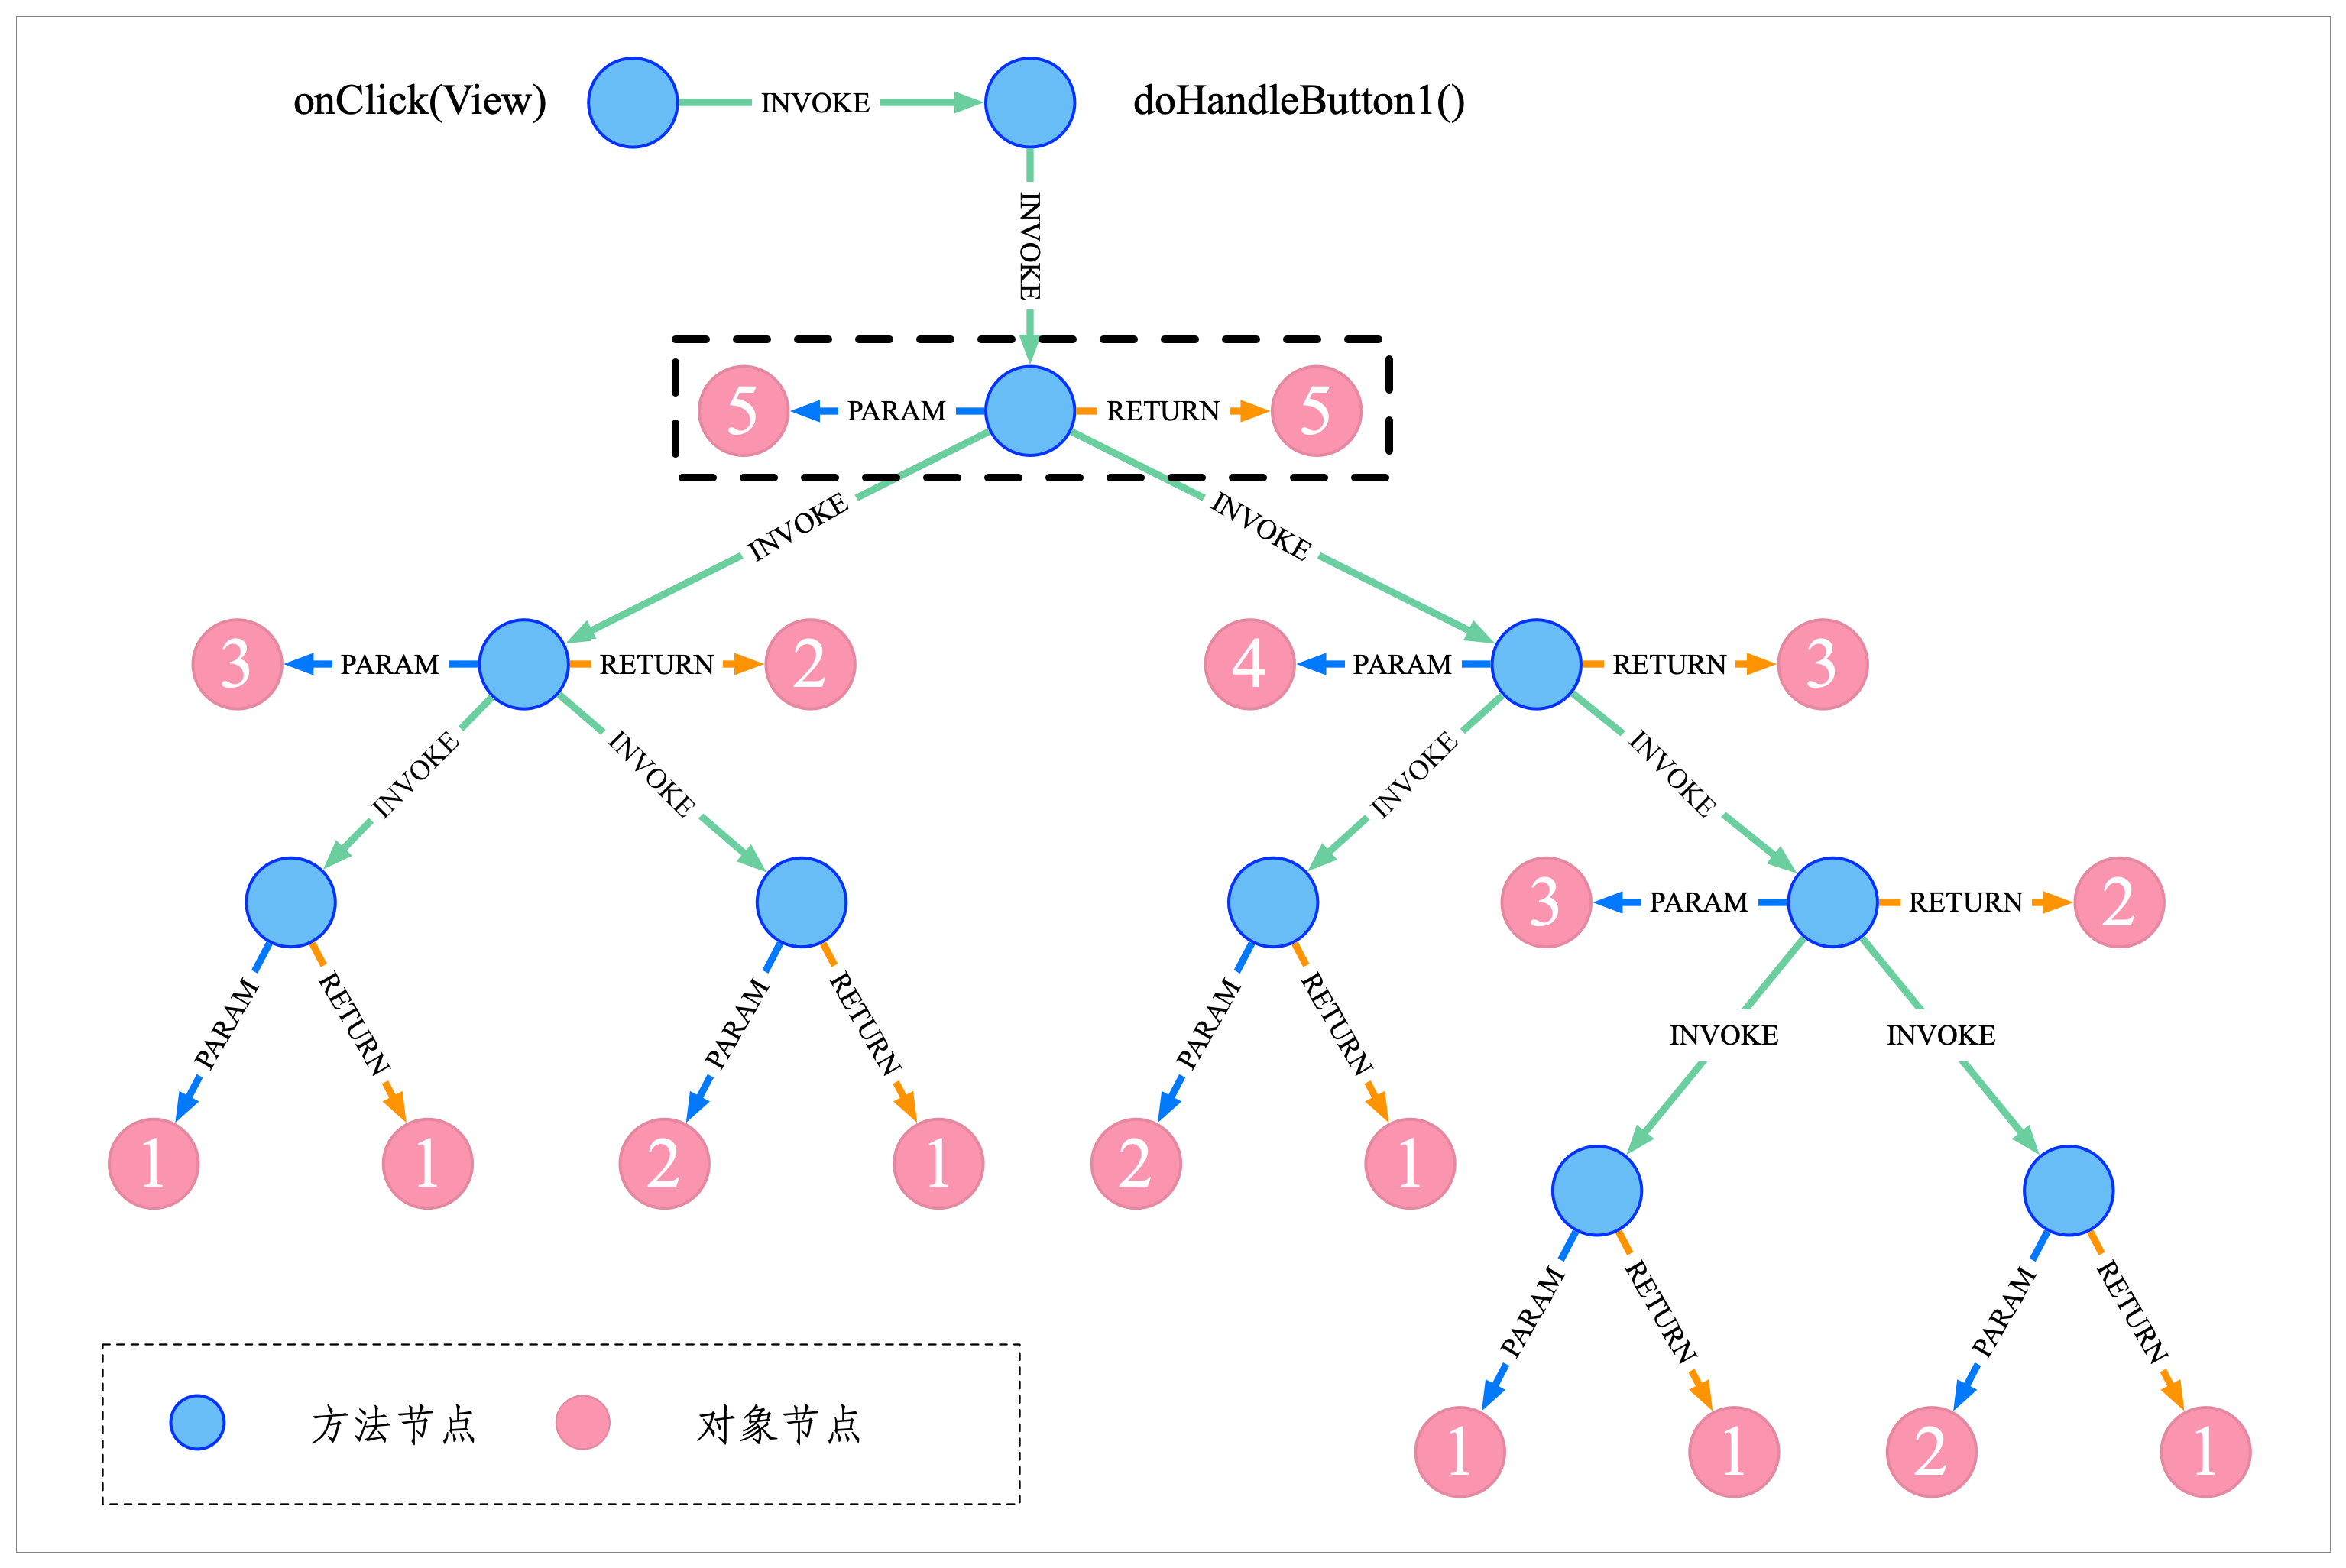
\includegraphics[width=\textwidth]{./Figures/doFibonacci-rundroid.png}
	\caption{斐波拉契数列相关的RunDroid调用图(局部)}
	\label{fig:rundroid-result-Fibonacci}
\end{figure*}
在本案例中,\code{doHandleButton1()}调用了方法\code{doFibonacci()},因此前者有条有向边指向后者;
通过观察虚线框中各节点的关系,我们知道,对于方法\code{doFibonacci()},当参数为5时,对应的结果为5。
FlowDroid的静态分析结果如\autoref{fig:flowdroid-result-Fibonacci}所示。
通过比较\autoref{fig:rundroid-result-Fibonacci}和\autoref{fig:flowdroid-result-Fibonacci},我们可以发现以下有趣的现象:


首先,两者在方法\code{doFibonacci()}数量上不同的:RunDroid得到的结果中,方法节点\code{doFibonacci()}共有9个,即在运行过程中,\code{doFibonacci()}被调用了9次。
由于在一个应用中,每个方法的方法签名是唯一的,所以FlowDroid给出的结果中\code{doFibonacci()}只有一个节点。该节点上存在一个指向自己的环,表示这个方法在执行过程中可能出现递归调用的情况。
%另外,静态分析方法(FlowDroid)在分析\code{doFibonacci()}这类方法时,对函数的执行上下文做出准确的判断,进而给出程序准确的运行时行为。
FlowDroid得到的函数调用图往往以方法体本身作为研究的基本单元,因此只能表示方法之间的可能存在调用关系,不能刻画具体的执行过程,而RunDroid的函数调用图可以细化方法执行之间的关系,详细地反映了程序执行的具体过程。




\begin{figure*}[!hb]
	\centering
	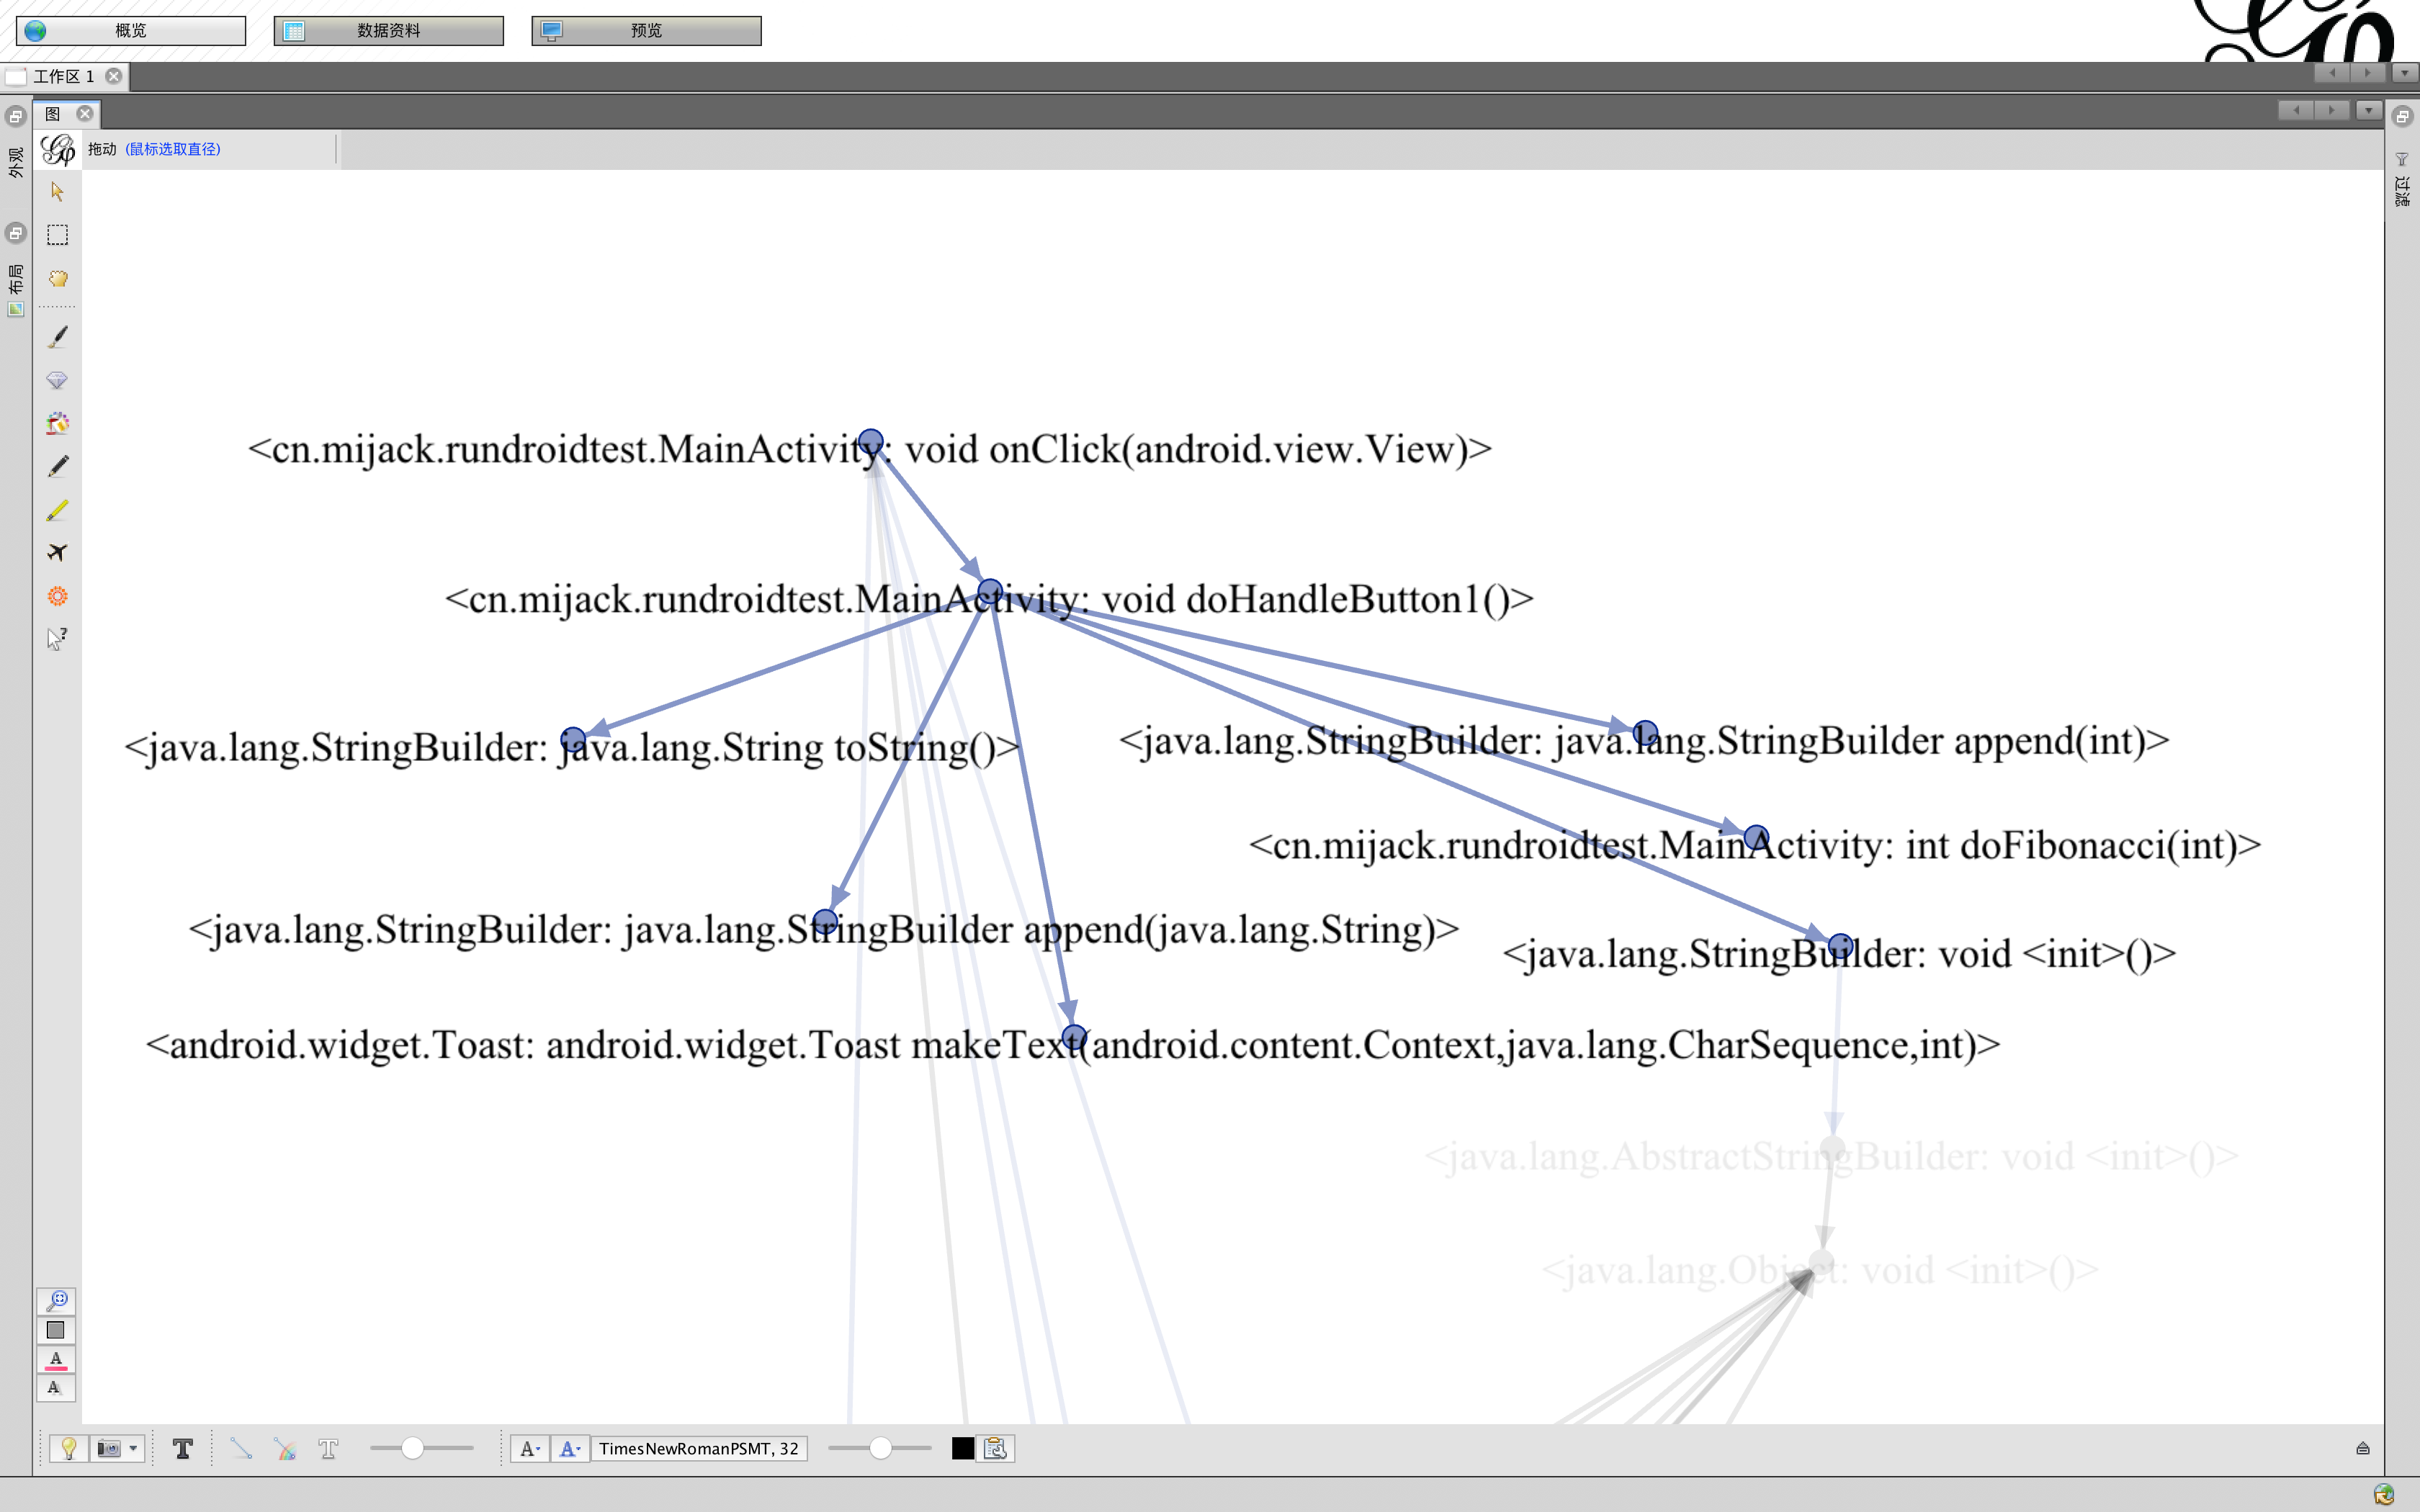
\includegraphics[width=\textwidth]{./Figures/FlowDroid-Fibonacci.png}
	\caption{斐波拉契数列相关的FlowDroid调用图(局部)}
	\label{fig:flowdroid-result-Fibonacci}
\end{figure*}


其次,在运行过程中,斐波拉契数列的计算结果最终以Toast的形式展现在界面上。
但方法\code{Toast.makeText(Context,CharSequence,int)}没有出现在RunDroid的结果中,却出现在FlowDroid给出的结果。
出现这个现象的原因如下:该方法属于系统定义的方法,而运行时拦截器待拦截的方法列表中并未包含该方法,因此运行时未收集到相关的方法执行信息,导致RunDroid无法在调用图中还原相应方法的方法执行。
这也反映了RunDroid的不足:关于系统函数的运行时信息的捕获需要提前将相应的方法告知运行时拦截器,生成的调用图才会包括相应的方法。
虽然RunDroid得到函数调用图缺失了部分方法,存在局部不完整,但是调用图中只包含研究人员关心的方法执行信息,突出研究重点,避免了分析信息的繁杂。



最后,FlowDroid给出的结果中包括了大量和{StringBuilder}相关的方法,而RunDroid的结果并不包括这些方法:
对比源码发现,源程序并未直接使用 {StringBuilder}。
通过查阅文献[\citenum{gosling2000java}],在编译过程中,Java编译器会通过对源代码做适当等价修改,通过引入{StringBuilder},避免表达式求值过程中产生过多的中间字符串对象,提高字符串连接的性能。
由于上述过程发生在Java程序编译阶段,并最后以字节码的形式保存在APK文件中,而FlowDroid从字节码层面对应用进行分析,因此FlowDroid的分析结果会包含该方法。
对于RunDroid,上述方法既在源代码中未出现相关方法定义(无法进行日志代码编织),又不在运行时拦截器的目标方法列表中,所以RunDroid给出的调用图自然也不会包括{StringBuilder}相关的方法。



\subsection{Activity 生命周期和事件回调的效果展示}


在本节中,应用运行时,我们将点击按钮button2,在{MainActivity}启动另一个{NewActivity},对比RunDroid和FlowDroid在Activity 生命周期和事件回调的效果展示。
最终,我们得到的RunDroid的运行结果如\autoref{fig:rundroid-result-lifecycle}所示。
针对Android 组件 {Activity}的生命周期特性,FlowDroid 进行了针对性的建模,将 Activity 的生命周期和UI事件回调串联起来,构造应用层面的方法\code{dummyMainMethod()}表示应用的执行过程,相应的结果如\autoref{fig:flowdroid-result-lifecycle}所示。


\begin{figure*}[!ht]
	\centering
	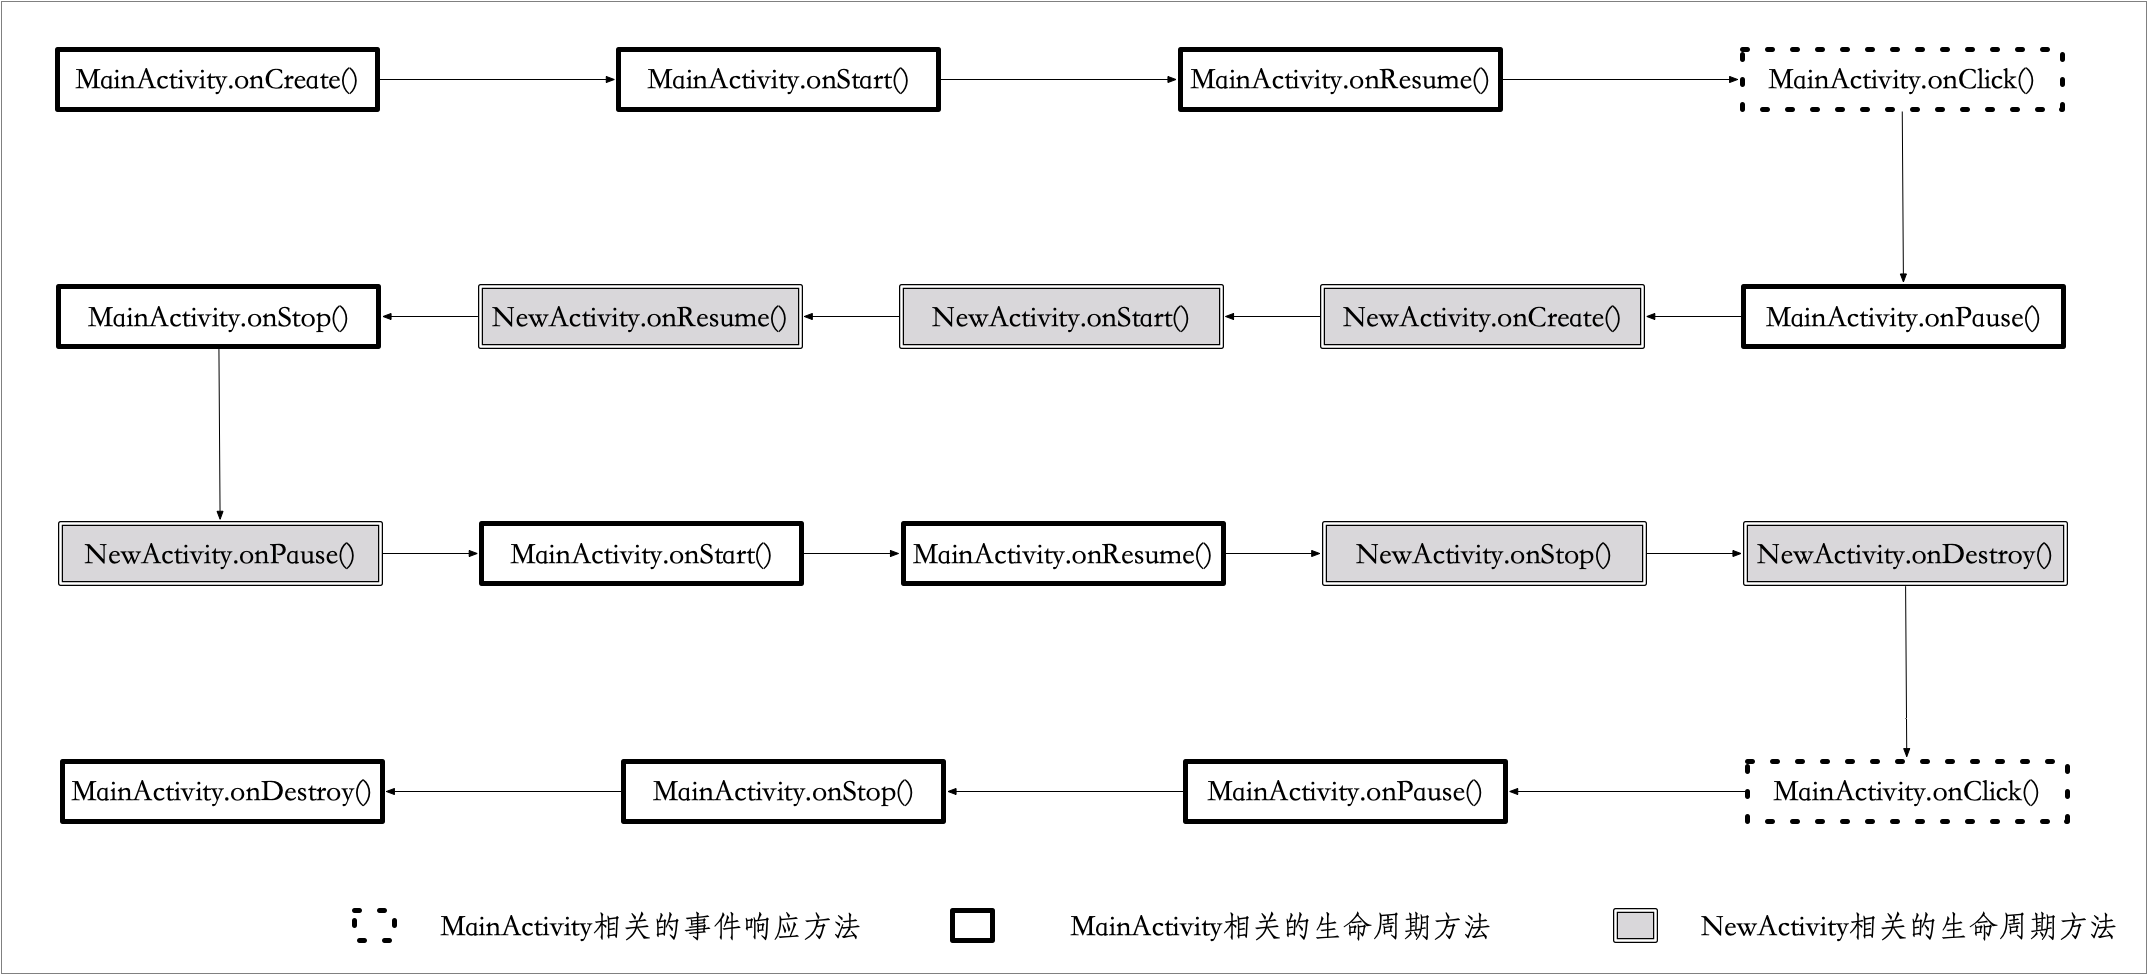
\includegraphics[width=\textwidth]{./Figures/android-lifecycle-rundroid.png}
	\caption{Activity生命周期和事件回调的RunDroid调用图(局部)}
	\label{fig:rundroid-result-lifecycle}
\end{figure*}


对比\autoref{fig:rundroid-result-lifecycle}和\autoref{fig:flowdroid-result-lifecycle},
我们可以发现RunDroid和FlowDroid在组件生命周期和事件回调上的设计思想上是不同的:
RunDroid可以捕获到组件生命周期方法以及回调事件方法的实际执行,因此,RunDroid对于上述行为的展现是按照时间的先后顺序将这些方法节点串联起来,形成完整的事件序列。
而FlowDroid在生成函数\code{dummyMainMethod()}时,会为AndroidManifest.xml文件中定义的每一个Activity单独创建包含生命周期方法和事件回调方法的状态迁移图
(\autoref{fig:flowdroid-result-lifecycle}中的虚线框部分表示每个Activity各自的整体状态迁移,灰色部分为{MainActivity}中的UI事件响应方法),
最后将这些Activity的状态迁移串联起来,并将Action为\code{android.intent.action.MAIN}并且category为\code{android.intent.category.LAUNCHER}的Activity组件作为结果的默认启动的Activity,最终形成方法\code{dummyMainMethod()}。


\begin{figure*}[ht]
	\centering
	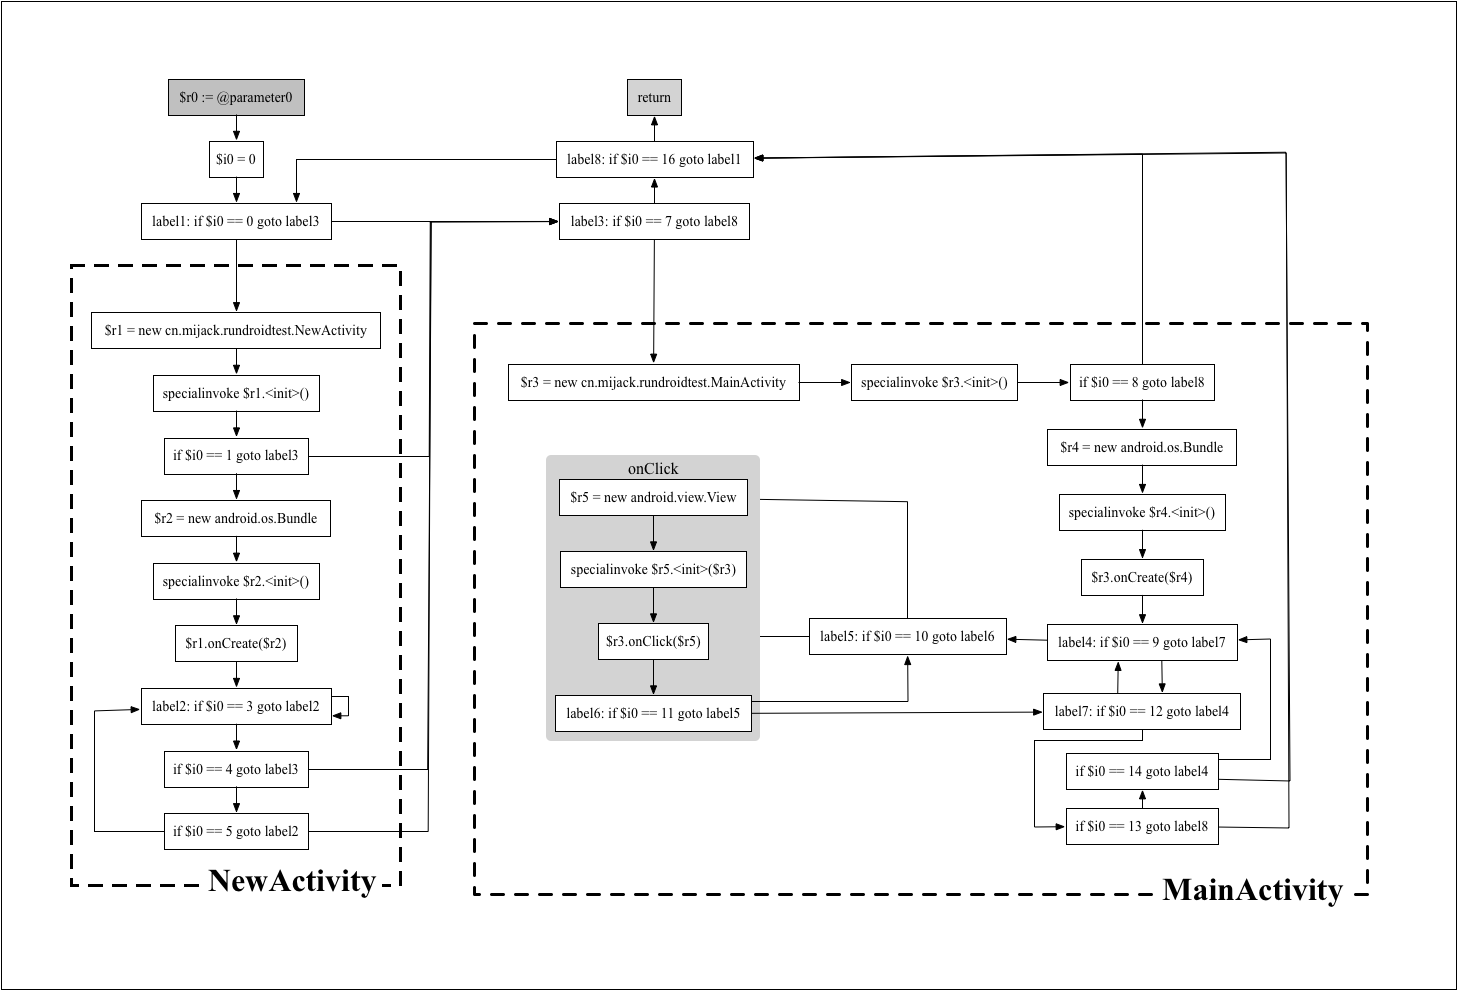
\includegraphics[width=\textwidth]{./Figures/flowdroid-dummyMainMethod.png}
	\caption{FlowDroid生成的函数dummyMainMethod()的调用图}
	\label{fig:flowdroid-result-lifecycle}
\end{figure*}

在结果展现上,RunDroid倾向于展现所有和Activity生命周期相关的方法。
例如,虽然开发人员在源代码中没有定义\code{onResume()}等方法,但在运行过程中,{MainActivity}的父类方法\code{onResume()}被调用了,便会出现在RunDroid的结果中。
而FlowDroid在这点上的处理方式恰恰相反:FlowDroid认为一个父类方法未被重写,则该方法运行行为表现保持一致性,FlowDroid并不会在结果中展示父类Activity未重载的生命周期方法。



另外,我们发现在应用从{MainActivity}切换到{NewActivity}过程中,
对应的生命周期变化为\code{MainActivity.onPause()} $\to$\code{NewActivity.onCreate()}$\to$\code{NewActivity.onStart()}$\to$\code{NewActivity.onResume()}$\to$ \code{MainActivity.onStop()},
{MainActivity}和{NewActivity}的生命周期方法是交替出现的,
并不是{MainActivity}的生命周期方法全部执行完毕后才执行{NewActivity}的生命周期方法。
而FlowDroid给出的结果将{MainActivty}和{NewActivity}分开处理,因此得到的结果属于后者。
相比FlowDroid,RunDroid的运行结果是程序运行时的直接反映,真实地反映了应用的状态变化。


\subsection{多线程触发关系效果展示}

多线程开发是Android开发中过程的典型开发要求。
本文针对此场景,我们进行了相关的测试。
在本节,我们将点击按钮button3,获取\code{doHandleButton3()}相关的调用图情况。
经过实验,RunDroid和FlowDroid的运行结果分别如\autoref{fig:rundroid-result-handler}、\autoref{fig:flowdroid-result-handler}所示。
两幅图在以下节点上存在不同。





\begin{figure*}[ht]
	\centering
	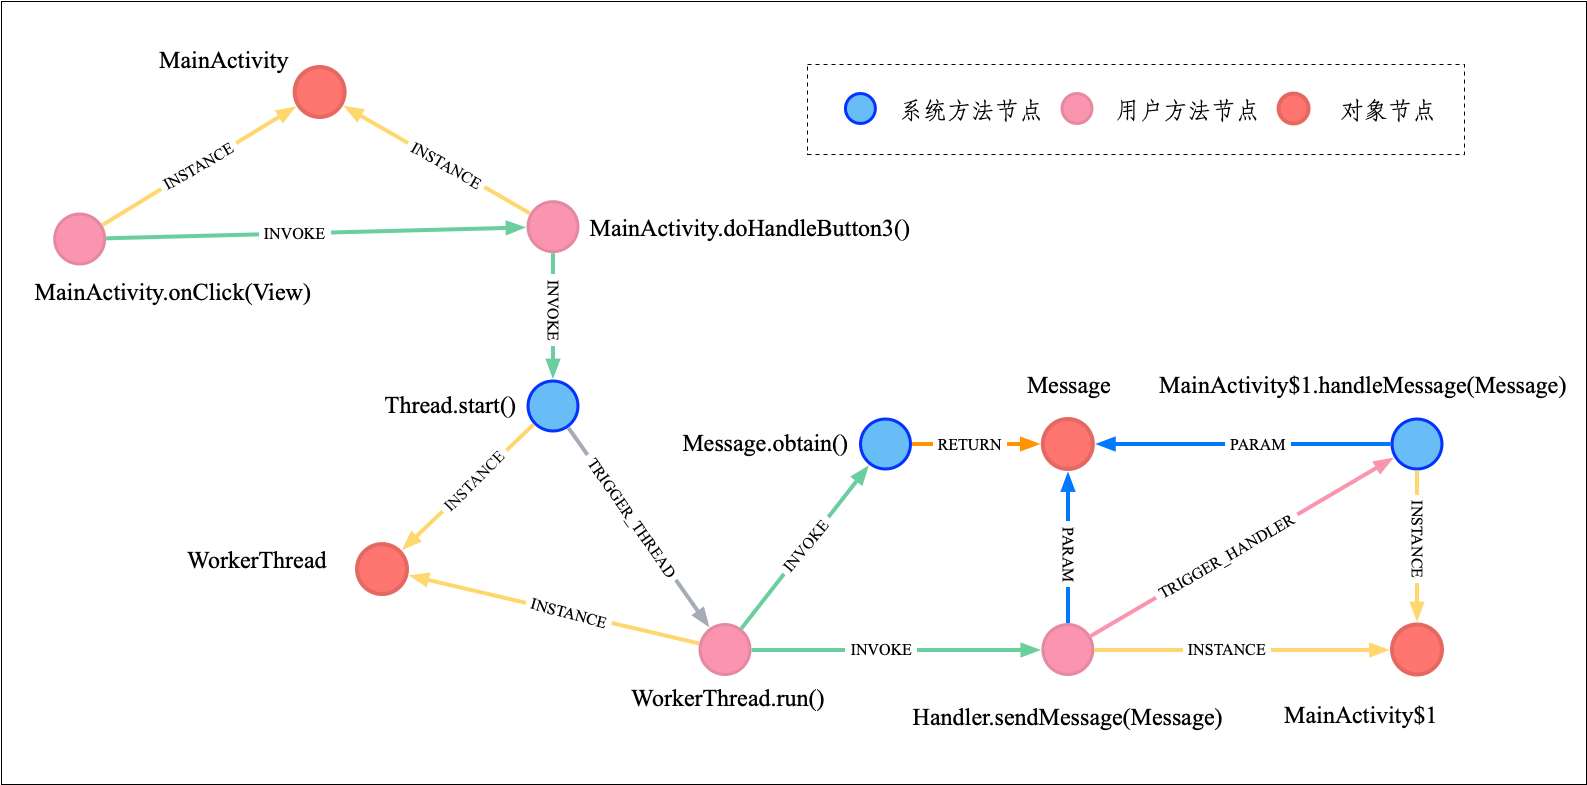
\includegraphics[width=\textwidth]{./Figures/android-handler-rundroid.png}
	\caption{多线程触发关系相关的RunDroid调用图(局部)}
	\label{fig:rundroid-result-handler}
\end{figure*}



\begin{figure*}[ht]
	\centering
	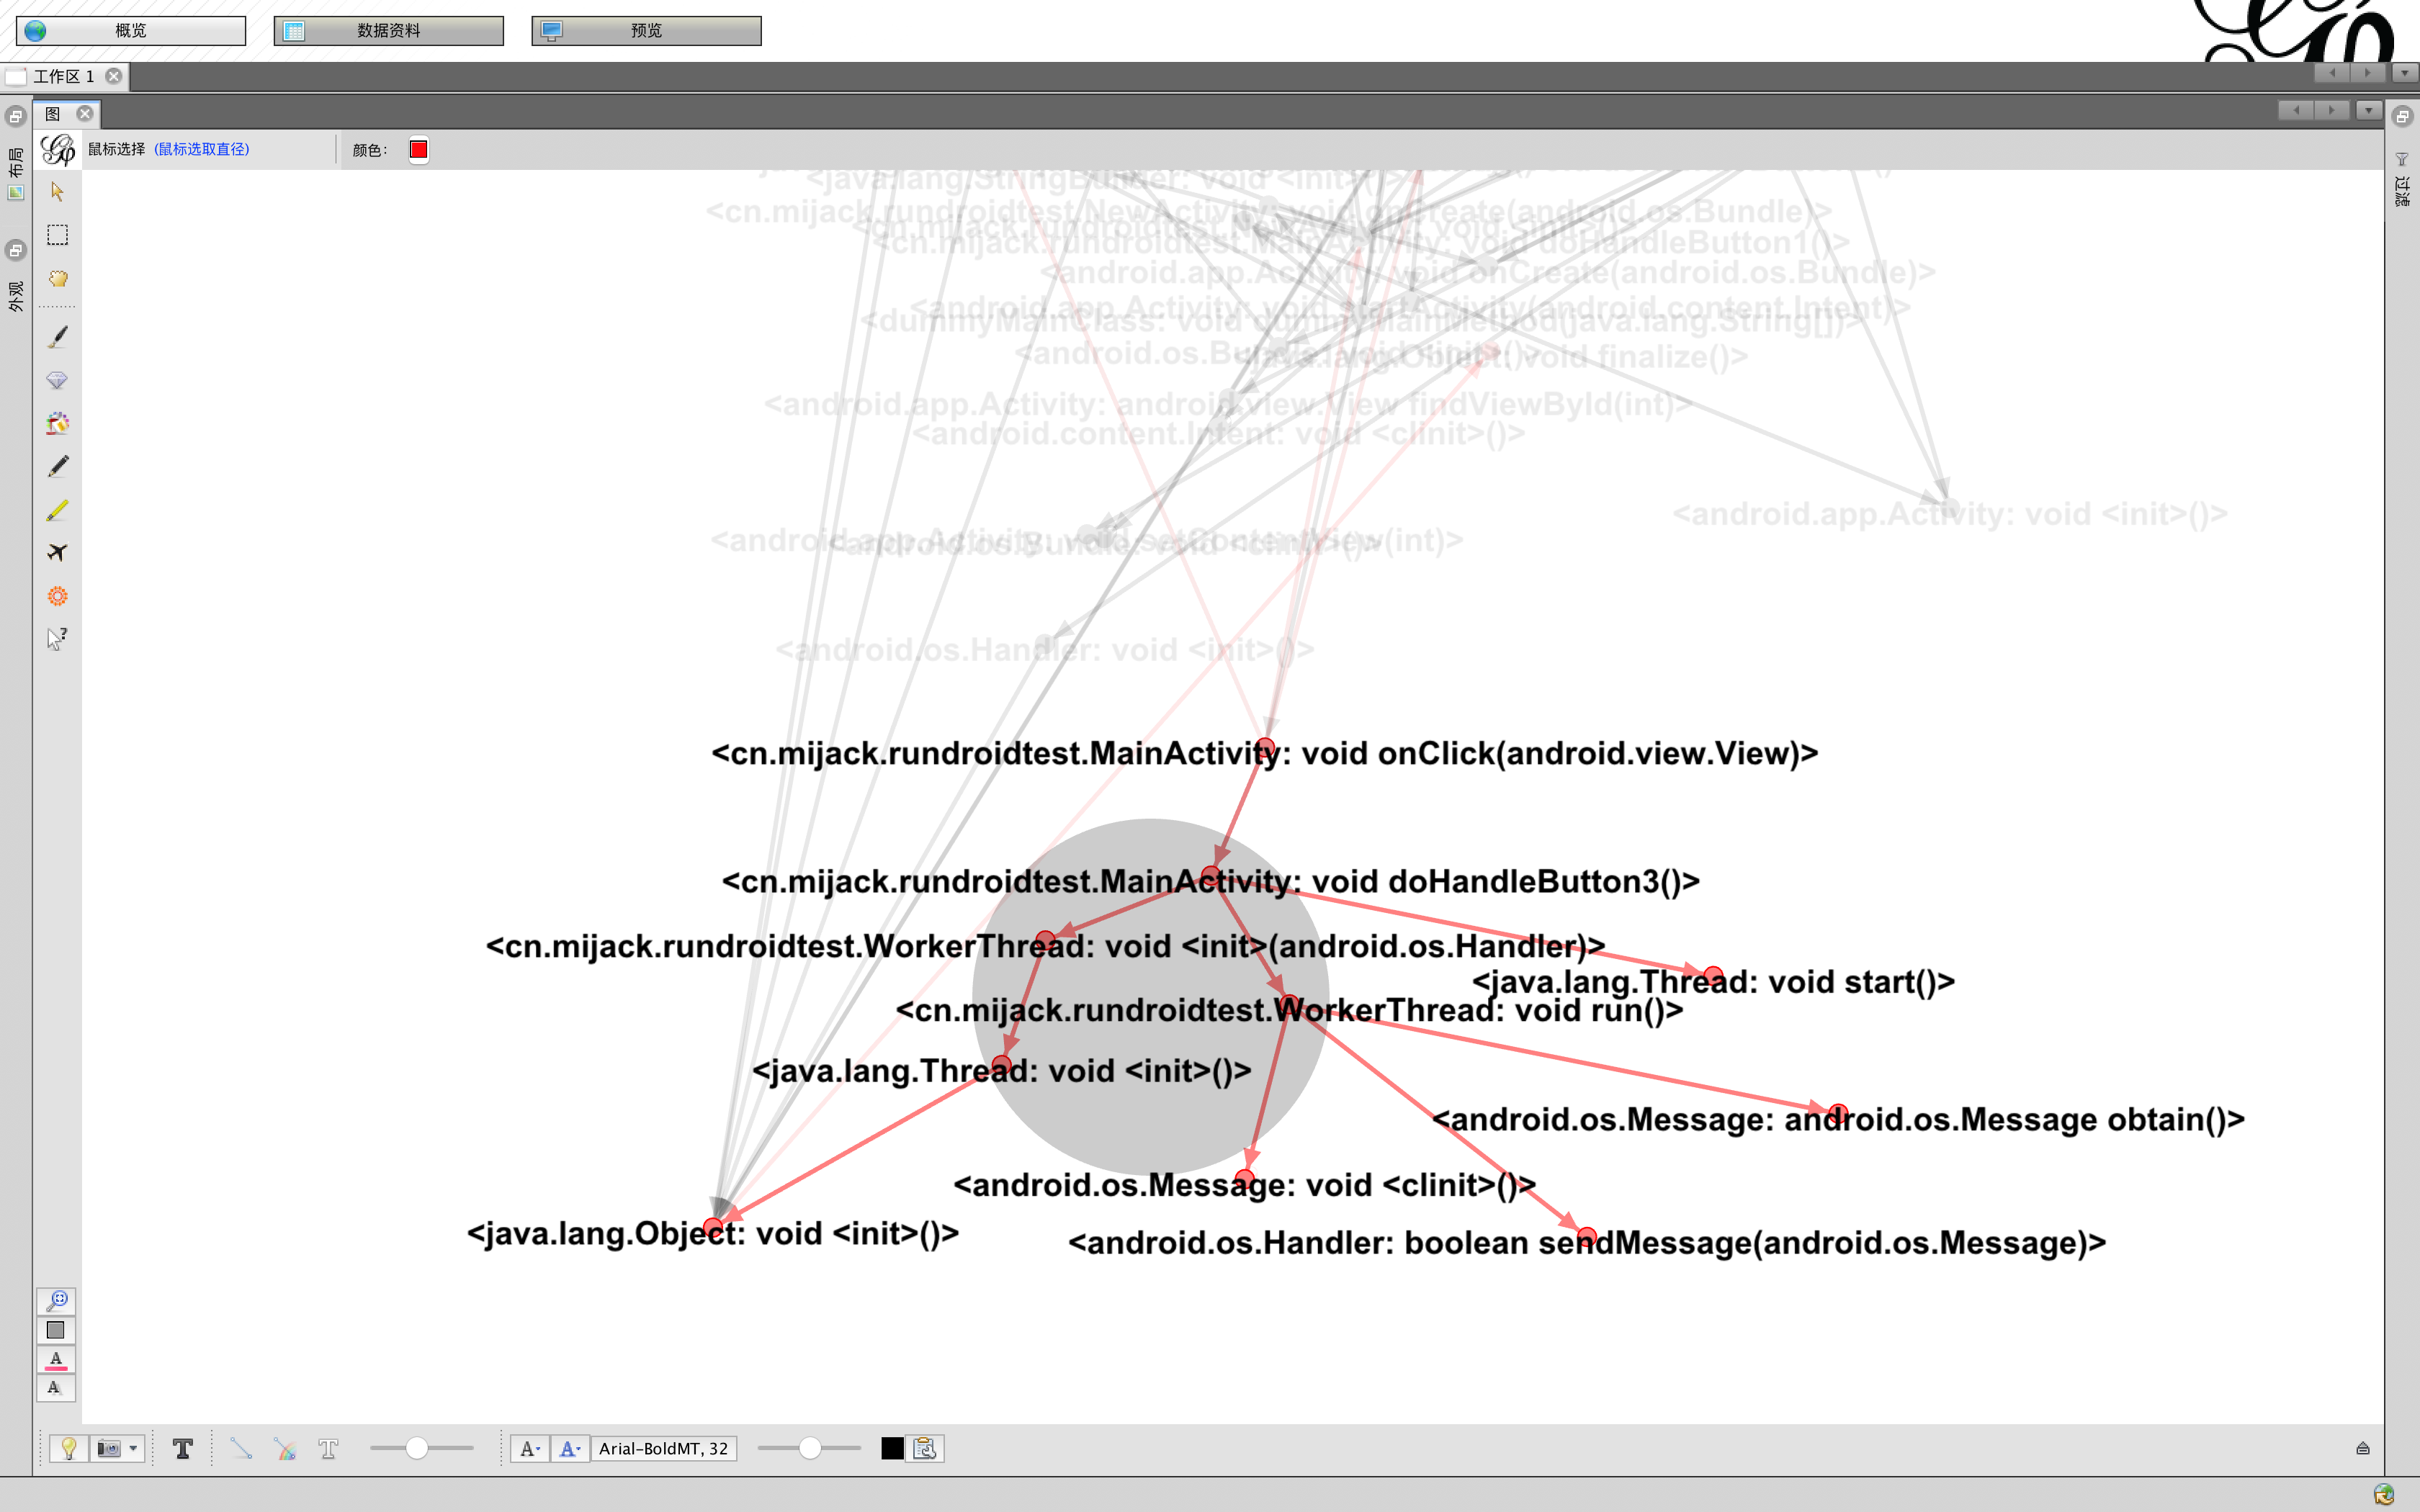
\includegraphics[width=\textwidth]{./Figures/FlowDroid-handler.png}
	\caption{多线程触发关系-FlowDroid生成的调用图(局部)}
	\label{fig:flowdroid-result-handler}
\end{figure*}




\point{Java API多线程的触发方式}

RunDroid在方法\code{Thread.start()}和方法\code{WorkerThread.run()}之间添加了一条有向边。
这条有向边从前者指向后者,表示方法\code{Thread.start()}的执行触发了方法\code{WorkerThread.run()}的执行,边上标识着触发原因(Thread,通过Thread方式触发)。
FlowDroid对方法\code{doHandleButton3()}进行推算出\autoref{fig:code_demo}第42行中的变量$workerThread$类型为\code{WorkerThread}。
同时,FlowDroid可以推算出方法\code{Thread.start()}的执行会导致方法\code{WorkerThread.run()}的执行。
在FlowDroid的设计者看来,方法\code{Thread.start()}可以替换成方法\code{WorkerThread.run()}。
因此,FlowDroid的结果中,方法\code{doHandleButton3()}和\code{WorkerThread.run()}之间存在调用边。
这条有向边并不是像RunDroid从\code{Thread.start()}出发。
虽然RunDroid和FlowDroid都可以在函数调用图表现Java API多线程的触发方式,但相比之下,RunDroid针对性地标识了函数间的关系,呈现方式更为全面严谨,更体现程序的运行过程。



\point{基于Handler的多线程触发方式}

在WorkerThread的方法run()中,我们通过Handler进行了异步UI操作,触发了方法\code{MainActivity\$1.handleMessage(Message)}的执行。
在构建拓展调用图过程中,RunDroid充分挖掘了这些方法和对应的方法对象的关联关系,进而补全方法\code{Handler.sendMessage()}和\code{MainActivity\$1.handleMessage(Message)}之间的触发关系。
因此,在RunDroid展示的结果中,上述两个方法之间存在一个从前者指向后者的有向边,边上标识着相应的触发原因(通过Handler方式触发,Handler)\footnote{由于我们定义的Handler是MainActivity的匿名内部类,因此编译后的类名为\code{MainActivity\$1}。}。
但是,FlowDroid分析相关代码时,由于缺少运行时上下文信息,无法分析出\code{WorkerThread.run()}中handler的具体类型,因此无法将这两个方法连接起来。




\point{静态方法的使用}


另外,在FlowDroid给出的结果中,我们发现方法\code{doHandleButton3()}还调用了类{Message}的类初始化方法\code{<clinit>()}。
原因是方法\code{doHandleButton3()}调用类\code{Message}的静态方法\code{obtain()},因此可能需要进行类的初始化。
由于在程序运行过中,方法\code{doHandleButton3()}在执行方法\code{Message.obtain()}前,类{Message}已经完成了类的初始化,方法\code{Message.<clinit>()}并没有被调用。
在RunDroid的结果中,上述两个方法不存在调用关系。
这从一个侧面方面反映出FlowDroid分析的结果和动态运行的过程可能存在一定的偏差。





\section{RunDroid在错误定位领域的应用}
在本节中,我们将采用因果关联模型\cite{baah2010causal,baah2011mitigating}作为错误定位技术。
相比传统错误定位技术(基于频谱的错误定位)只考虑了程序语句的覆盖情况,基于因果关联模型的错误定位技术还考虑程序在执行过程中的程序依赖(即控制依赖和数据依赖),分析的准确度较高。



\begin{equation}
\begin{aligned}
\tau(s) = E[Y=1|T=1] - E [Y=0|T=0] 
\end{aligned}
\label{equ:expectEquation} 
\end{equation}
\begin{scriptsize}
	注:$E[Y=1|T=1]$:实验组执行失败的期望, $E[Y=0|T=0]$:对照组执行通过的期望。
\end{scriptsize}


\begin{equation}
\begin{aligned}
Y =\alpha +\tau T+\beta X 
\end{aligned}
\label{equ:linearEquation} 
\end{equation}
\begin{scriptsize}
	注:其中$Y$表示测试用例是否执行失败(1为执行失败,0为执行通过),
	$T$和$X$分别为语句$s$和$Pred(s)$中各语句的覆盖情况 ,
	$\beta$ 为$Pred(s)$中各语句的错误估计值,$\alpha$ 为公式中待计算的定值。  \par
	
\end{scriptsize}

\subsection{原理简介}



基于因果关联模型的错误定位技术,以程序本身$P$和程序在一组测试用例下的覆盖率信息作为输入,
通过期望模型(\autoref{equ:expectEquation})和线性回归模型(\autoref{equ:linearEquation})计算程序$P$中的语句$s$的相应的错误估计值$\tau$。
$\tau$的值越大,语句$s$是错误的可能性越大。
具体过程如\autoref{alg:fault-localization}所示。


\begin{algorithm}[!ht]
	
\tablewuhao

\caption{错误定位的计算方法} 


\label{alg:fault-localization}
\KwIn{ $P$,应用程序}
\KwIn{ $CoverageInfo$,应用程序的覆盖信息}
\KwOut{ $sorted\_\tau$,程序语句的逆向排序}


\SetKwProg{Fn}{Function}{:}{}

\Fn{FaultLocazilation($P$,$CoverageInfo$)}{
	
	\For{$s \in P$ }{
		
		计算语句$s$在程序$P$中前驱节点集合$Pred(s) $;
		
		根据$Pred(s) $的覆盖率情况筛选待计算的数据$Mdata(s)$;
		
		\eIf{\emph{$Mdata(s)$ 为 $\emptyset$	}}{
			使用$Mdata(s)$根据\autoref{equ:expectEquation}计算 $\tau(s)$ ;			
		}{
			根据\autoref{equ:linearEquation}计算 $\tau(s)$ ;
		}
		
	} 
	
	对各语句按照$\tau$ 逆向排序得到	$sorted\_\tau$;
	
	\KwRet{$sorted\_\tau$};
	
}

\end{algorithm}






对于语句$s$,语句$s$的前驱节点集合$Pred(s)$指的是语句$s$在程序$P$中的控制依赖和数据依赖的合集(第3行)。
在匹配过程中,每个测试用例按照语句$s$前驱节点集合$Pred(s)$的覆盖率情况表示成一维向量,并按照语句$s$是否覆盖将测试用例分为实验组和对照组
(实验组(T=1)和对照组(T=0)分别与覆盖语句$s$的测试用例、未覆盖语句$s$的测试用例对应);
如果向量表示结果相同的测试用例同时出现实验组和对照组中,则保留对应的测试用例到集合$Mdata(s)$中,反之不保留(第4行)。
匹配完毕后,当$Mdata(s)$不为空集,我们将使用\autoref{equ:expectEquation}计算语句$s$的错误估计值$\tau(s)$(第6行)。
当$Mdata(s)$为空集,我们将通过线性回归\autoref{equ:linearEquation}公式计算得到关于$T$的斜率$\tau$作为语句$s$的错误估计值$\tau(s)$(第8行)。
最后,对于所有的语句,按照错误估计值逆向排序输出,算法完毕。

%以\Line{5}为例,\autoref{tab:result}代码中\Line{5}的控制依赖语句是\Line{4},数据依赖节点是\Line{2},因此$Pred(\Line{5}) = \{ \Line{2}, \Line{4}\}$。
%测试用例$t_1 \sim t_5$对应的$Mdata(s)$分别表达成$V_{t_1}=\langle1,0\rangle$、$V_{t_2}=\langle1,1\rangle$、 $V_{t_3}=\langle1,1\rangle$、 $V_{t_4}=\langle1,0\rangle$、$V_{t_5}=\langle1,1\rangle$。
%其中,测试用例$t_1$、$t_2$、$t_4$、$t_5$为实验组,$t_3$为对照组。
%由于只有向量$\langle1,1\rangle$同时出现在实验组和对照组,所以测试用例$t_2$、$t_3$、$t_5$保留到$Mdata(\Line{5})$中。
%根据\autoref{equ:expectEquation}计算可得$\tau(\Line{5}) = \frac{0+0}{2}-\frac{1}{1}=-1$。
%而对于\Line{2},该语句并没有前驱节点,匹配完的集合$Mdata(\Line{2})$为空集,因此通过\autoref{equ:linearEquation}对所有测试用例的数据进行计算。
%由于结算结果中回归直线斜率不存在,所以$\tau(\Line{2})= \text{NA}$。


\subsection{结果分析}


为了验证RunDroid提供的动态调用图对因果影响模型有一定的提升作用,
我们按照[\citenum{baah2010causal,baah2011mitigating}]的实验设置,使用原始因果影响模型的计算结果(没有RunDroid)作为基线,和并使用RunDroid后的因果影响模型的计算结果进行比较。
我们的实验对象如\autoref{tab:result}所示,代码\Line{13}为程序的错误(方法\code{loadData(int)}的参数不可为负数)。
在编写的5个测试用例$t_1\sim t_5$中,$t_2$、$ t_5$未通过测试。
列$\tau$为未使用RunDroid情况下的计算结果,列$\tau'$为使用RunDroid情况下的计算结果。

\begin{table}[!ht]
	
	\caption{结果对比}

	
	\label{tab:result}
	\begin{center}
		\scriptsize	
		
		
		
		\begin{tabular}{|rl*{5} {|c}|c|c|}
			
						\hline
			
			&                    & $t_1$ & $t_2$ & $t_3$ & $t_4$ & $t_5$ & ~&  ~\\
			&v &btn0& btn1& btn1& btn2 &btn1 & $\tau$ &  $\tau'$   \\
			&num&   - & - 1& 0& -& -2& &\\
			\hline
			
			\Line{~1}&void onClick(View v) \{                       &   &   &   &   &   &      &         \\
			
			\Line{~2}&\quad num = getNumber();                   & 1 & 1 & 1 & 1 & 1 &  NA  &  NA    \\
			
			\Line{~3}&\quad if(v.getId() == R.id.btn1) \{           & 1 & 1 & 1 & 1 & 1 &  NA    &  NA \\
			
			\Line{~4}&\quad \quad if( num == 0 ) \{                    & 0 & 1 & 1 & 0 & 1 & 0.67   & 0.67 \\
			
			\Line{~5}&\quad \quad \quad num=1;                         & 0 & 0 & 1 & 0 & 0 & -1.0  &-1.0\\
			
			\Line{~6}&\quad \quad \}                                   &   &   &   &   &   &       &            \\
			
			\Line{~7}&\quad   \}                                       &   &   &   &   &   &      &            \\
			
			\Line{~8}&\quad Thread t = createThread(v.getId());          & 1 & 1 & 1 & 1 & 1 & NA&  NA  \\
			
			\Line{~9}&\quad t.start();                                 & 1 & 1 & 1 & 1 & 1 & 0.67   & 0.67 \\
			
			\Line{10}&\}                                              &   &   &   &   &   &      &             \\
			
			\Line{11}&TaskThread.run() \{                             &   &   &   &   &   &      &       \\
			
			\Line{12}&\quad if(v.getId() == R.id.btn1) \{                          & 1 & 1 & 1 & 1 & 1 &  NA   & NA \\
			
			\Line{13}&\quad \quad \textbf{loadData(num); /* FAULT */} & 0 & 1 & 1 & 0 & 1 & 0.67    & 1.0  \\
			
			\Line{14}&\quad\}                                         &   &   &   &   &   &  &                \\
			
			\Line{15}&\}                                              &   &   &   &   &   &   &              \\
			
			\hline
			
			&                                                  & 0 & 1 & 0 & 0 & 1 &   &               \\
									\hline
		\end{tabular}
	\end{center}
\wuhao
	注: 第2列到第6列分别代表测试用例$t_1\sim t_5$;
	每个测试用例列的标题分别显示在第1行和第2行使用的v和num的值;
	测试用例列的值指示相应的程序语句是否由测试用例执行,1表示覆盖,0表示未覆盖;   
	最后一行表示各个测试用例的执行结果,“1”表示测试未通过($Y=1$),“0”表示测试通过($Y=0$)。  \par
	
	
\end{table}





在$\tau$的结果中,分数最高包括\Line{4}、\Line{7}和\Line{13},均为0.67;
在$\tau'$的结果中,分数最高只有\Line{13},分数从原来的0.67提升到1。
而其他行的分数保持不变。
在RunDroid接入后,错误语句的分数有所提高,同时错误语句与非错误语句得到区分。
因此,$\tau'$的结果比结果$\tau$更好。


\begin{figure}[!ht]
	\begin{center}
		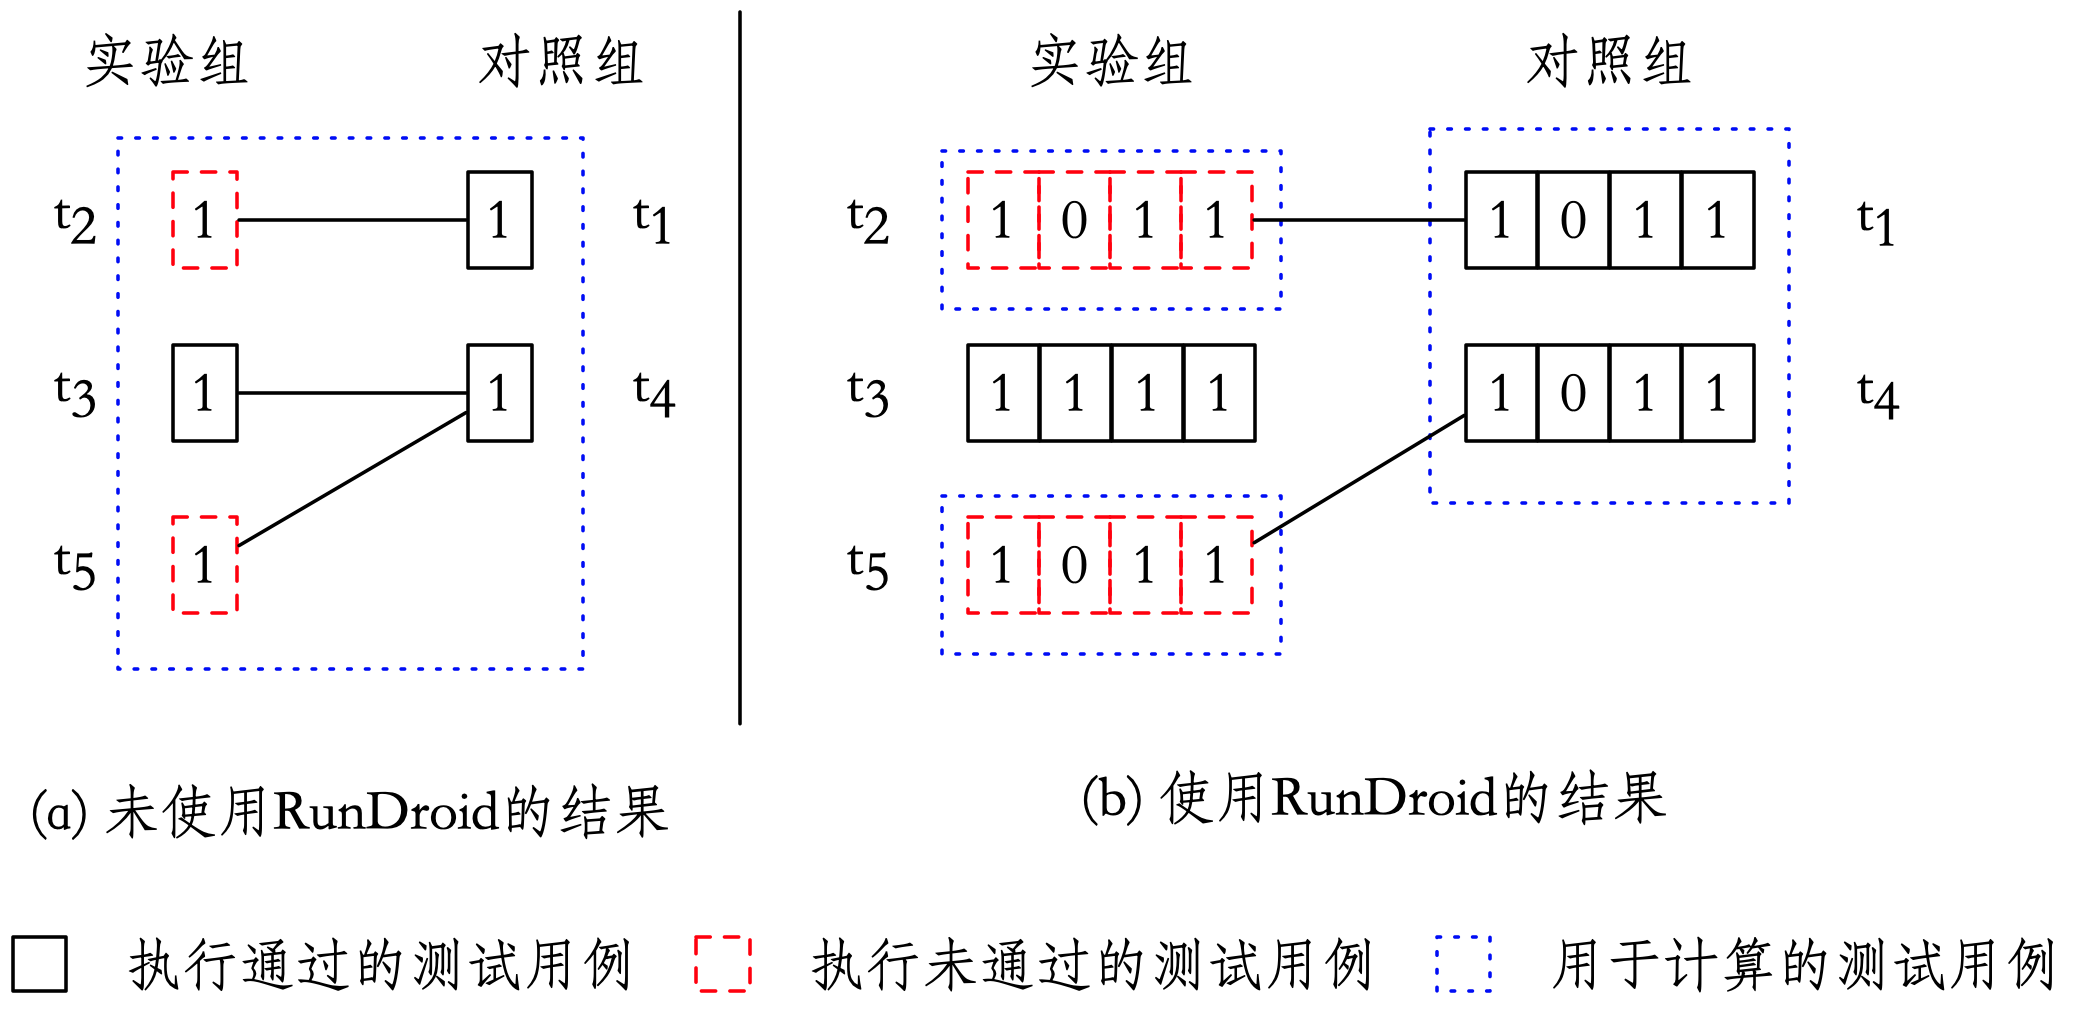
\includegraphics[width=0.8\textwidth]{./Figures/fault-localization.png}
	\end{center}
	\caption{使用RunDroid前后关于语句\Line{13}的测试用例匹配的对比}
	\label{fig:motivationResultTreatment}
\end{figure}


\Line{13} 分数提高的原因如下:
在接入RunDroid前,方法\code{onClick(View)}和\code{TaskThread.run()}没有任何调用关系。
因此,\Line{13}的前驱节点集合中只包括控制依赖语句\Line{12} ,实验组和对照组的$Mdata(\Line{13})$数据如\autoref{fig:motivationResultTreatment}-(a)所示,所有的测试用例参与计算:$\tau= \frac{1+1+0	}{3} - \frac{0+0}{2} = 0.67$。
而接入RunDroid后,方法\code{onClick(View)}和\code{TaskThread.run()}通过方法触发关系产生方法间的因果关联,进而形成新的程序依赖关系。
\Line{13}的前驱节点增加了\Line{2}、\Line{5}和\Line{9},变为$\{ \Line{2},\Line{5},\Line{9} ,\Line{12}\}$,实验组和对照组的$Mdata(\Line{13})$如\autoref{fig:motivationResultTreatment}-(b)所示。
实验组中的测试用例$t_3$在对照组中找不到对应的测试用例,因此不参与计算。
最后,根据测试用例$t_1$、$t_2$、$t_4$、$t_5$得到\Line{13}的错误估计值:$\tau =  \frac{1+1	}{2} - \frac{0+0}{2} = 1$。
\Line{12}的前驱节点也发生了变化,但是由于实验组和对照组匹配结果保存不变,因此结果保存不变。
而对于其他语句,前驱节点的信息并没有发生变化,因此数值保持不变。



%RunDroid提供的函数调用图中不仅仅包括函数调用关系,还包括函数触发关系,两者均可以表示方法执行的因果关系。
RunDroid提供的动态调用图,从方法调用关系和方法触发关系两个方面反映方法间的因果关系,辅助补全函数间的控制依赖和数据依赖。
相比之前的技术只从函数调用角度分析程序,RunDroid辅助下的程序分析结果更为全面,对因果影响模型有一定的提升作用。
因此,RunDroid和错误定位技术的结合能使得结果得到一定的提升。

\eat{

在\autoref{tab:result}中,我们在第13行显示了一个错误的语句示例。
而是直接传递,如果在传入方法之前它是一个正值,则应检查第13行的方法loadData(int)的参数。
第一列显示了与每个语句关联的行号的程序假设我们使用因果影响模型计算程序的失效原因,我们能够计算列“结果”中显示的估计数。第4,9和13行都是估计的,得分最高为0.67。
}
\eat{
	
	In Table 1, we show an example faulty program with a faulty statement at Line 13. 
	Instead being passed directly, the parameter of method loadData(int) at Line 13 should be checked if it is a positive value before passing into the method. 
	The first column shows the program with line numbers associated with each of its statements.
	Columns 2 through 6 represent test cases t1-t5, respectively. 
	The header of each test case column shows the values of v and num that are used at Lines 1 and 2, respectively. 
	The values for a test case column indicate whether the corresponding program statement is exercised by the test case, 1 for covered and 0 for not covered. 
	The bottom row shows the outcome of each test case execution, with “1” indicating a failing execution and “0” indicating a passing one.
	Suppose we compute the failure-causing effect of the program using the causal influence model [7, 8], we are able to compute the estimate numbers shown in Column “result”. Lines 4, 9, and 13 are all estimated with the highest score 0.67.
}



\eat{
因果影响模型以及许多其他故障定位技术考虑了动态程序依赖的影响,因为依赖信息不仅有助于触发故障的影响,而且还将它们传播到程序输出。
不幸的是,由于Android的特定编程范例,在显示的示例中无法捕获第8行和第11行之间的控制依赖性。
并且,丢失适当的控制流导致计算报告具有相同最高分的三个语句,从而使得故障定位技术在Android中不那么有效。
因此,为了改进Android应用程序的故障定位技术,RunDroid旨在通过运行时信息和执行期间的动态调用图来恢复非常需要的控制流依赖性。

}

\eat{



我们将激励性的例子作为主题计划。
因果影响模型在很大程度上依赖于陈述之间的依赖关系。
使用RunDroid,捕获了第9行\code{t.start()}和第11行\code{TaskThread.run()}之间的异步触发关系,因此第13行的前导是行$ \{ $ 5,8,9,13 $ \} $,而不仅仅是第13行,这是原始因果影响模型的情况。
\autoref {fig:motivationResultTreatment}显示治疗单位和控制单位及其相关的第13行测试用例。
具体来说,\autoref {fig:motivationResultTreatment} - (a)代表没有RunDroid的情况,而\autoref {fig:motivationResultTreatment} - (b)代表RunDroid的情况。
治疗单位是第13行的测试用例,分别为$ t_2 $,$ t_3 $和$ t_5 $;控制单元是不包括第13行的测试用例,是$ t_1 $和$ t_4 $。
对于目标语句,我们使用协变量向量在测试用例中显示其前任语句的封面信息。
显示了由测试用例生成的协变量值的向量。
在\autoref {fig:motivationResultTreatment} - (b)中,向量$ \langle $ 0,1,1,1 $ \rangle $表示对于测试用例$ t_2 $,只包含第5行,其他三个前任语句(第8,9,12行)都包括在内。
使用来自因果推理模型的相同方程,后一种情况的因果效应估计(来自RunDroid的依赖信息)的结果不同。
第13行的估计是$ \frac {(1 + 1)} {2} - \frac {(0 + 0)} {2} = 1.0 $。其他陈述的估计数见最右列表2。


}
	\eat{
		
		We take the motivating example as the subject program.
		Causal influence model relies heavily on dependence relationship among statements.
		With RunDroid, the asynchronized trigger relation between Line 9 \textit{t.start()} and Line 11 \textit{TaskThread.run()}, is captured, hence the predecessors of Line 13 are Lines ${\{}$5, 8, 9, 13$\}$, instead of Line 13 only, which is the case of original causal influence model.
		\autoref{fig:motivationResultTreatment} shows the treatment units and the control units with their associated test cases for Line 13.
		Specifically, \autoref{fig:motivationResultTreatment}-(a) represents the case of without RunDroid, and \autoref{fig:motivationResultTreatment}-(b) represents the case with RunDroid.
		The treatment units, which are test cases that cover Line 13 are $t_2$, $t_3$, and $t_5$; the control units, which are test cases that do not cover Line 13 are $t_1$ and $t_4$.
		For target statement, we use the vector of covariate to present the cover information of its predecessor statements in a test case.
		The vector of covariate values generated by the test cases is shown.
		In \autoref{fig:motivationResultTreatment}-(b), the vector $\langle$0,1,1,1$\rangle$ means that for test case $t_2$, only Line 5 is not covered, the other three predecessor statements (Lines 8, 9, 12) are all covered.
		Using the same equation from causal inference model, the causal-effect estimates for the latter case (with dependence information from RunDroid) are resulted differently. 
		The estimate for Line 13 is $\frac{(1+1)}{2}-\frac{(0+0)}{2} = 1.0$. The estimates for the other statements are shown in Table 2, in the far right column.
		
	}
	
	



\section{本章总结}
	


我们从开源社区F-Droid中下载9个开源应用程序,利用RunDroid产生这些应用程序的动态函数调用图,统计图中的函数触发关系。
我们发现函数触发关系(事件回调、Java 多线程以及Handler)普遍存在于应用程序的业务中,特别是Handler机制在Android应用程序中的使用尤为广泛。

% 本章中,我们将环绕着构建效率、日志效率、运行效率等三个方面对RunDroid角进行系统性能测试和评估,并结合实验结果阐述了采用源代码插桩、基于MMap的日志方案等原因。


我们将RunDroid产生的动态函数调用图和FlowDroid产生的静态函数调用图进行对比分析。
我们发现,RunDroid生成的调用图的完整性依赖于源代码处理以及待拦截的目标系统方法列表的完整程度,而FlowDroid的分析对象是Android应用程序APK文件,调用图的完整性受到自身算法实现的限制。
另外,两者在设计思想上不同的,RunDroid关心的是在程序执行过程中的方法之间的依赖关系,而FlowDroid则是站在函数调用可能性的角度,体现两个方法(包括递归调用)之间是否存在调用的可能性。
前者是某一应用运行的具体、微观的表现,而后者更多的是反映方法调用关系在宏观、理论上的可能性。
综上,RunDroid和FlowDroid体现方法的调用关系上各有千秋。


同时,我们将RunDroid和错误定位技术结合,进行了探索性的实验。
实验结果显示,RunDroid生成的调用图中的方法触发关系可以将异步方法调用(例如Java 多线程和Handler)关联起来,补全函数间的控制依赖和数据依赖关系。
在RunDroid提供的信息的帮助下,基于因果模型的错误定位技术相关实验结果得到一定的提升,提高了实验结果的准确度。

\clearPaperPage

\input{chapter-application.tex}
\clearPaperPage

\chapter{总结与展望}
\label{chp:future}

\section{总结}
% In this paper we first introduce the concept of fake apps, and study specifically towards these apps.
在本文中,``仿冒应用''这个概念被率先引入。
然后,本文对这一方面进行了专门的研究,还搜集了大量的相关样本以辅助调查。
% To the best of our knowledge, we are the first to conduct a comprehensive empirical study on a large-scale fake apps.
本文的前期调研结果显示,本课题是第一个针对仿冒应用进行大规模全面实证研究的课题。

% To better understand the ecosystem nature of this type of apps, we obtained more than 150,000 data entries from real-world markets, observed and measured the fake samples among this dataset from several dimensions including certificate information, app size, app name and package name, time factor and so on.
为了更好地了解这个类型的应用的生态环境,本文基于Python 3设计实现了仿冒应用收集框架\mytool,利用基于BFS的算法收集了来自现实世界中各个应用市场的近14万个应用样本,并且从多个不同维度,对这个数据库里面的仿冒样本进行了观测和考察。
这些维度包括了APK包中的安全证书信息、应用大小、应用名、包名和时间因素等等。

% Through our measurements we gain valuable experience on fake apps from several perspectives, findings like fake samples' naming tendency and fake developers' evasive strategies are inferred.
然后,本工作将收集到的数据分为了\emph{仿冒应用的基本特征}、\emph{影响仿冒应用数量的因素}和\emph{仿冒应用的发展轨迹}三个不同视角进行了测量,获得如仿冒应用的命名倾向和仿冒应用开发者对市场监管防御机制的规避策略等信息。
% To support our findings, we further present a few study cases which provide us a more detailed look into fake apps to back our discoveries on fake app ecosystem.
为了佐证本文的发现,本研究在每个视角解读之后给出了从数据集中挑选的几个研究案例,呈现了如仿冒应用开发者对不同热门应用的仿冒方式的内容。
这几个案例进一步深化了本文对仿冒应用生态系统的发现。

之后,本文还收集了部分仿冒样本在商场上对应的评论和评级,排查仿冒应用是否利用了排名欺诈。
由于现有的排名欺诈检测手段尚有不足,本工作创新性地分别利用两种创新的研究方法---基于用户行为的用户可信度验证和基于NLP的评论内容相似度验证,对数据中的排名欺诈行为进行了排查。
结果显示,刷好评的排名欺诈行为的确存在于应用市场中,在本工作搜集到的仿冒应用评论中就有刷好评的痕迹。


\section{展望}

在大规模分析的部分中,本文中用到了三个不同的角度分别探索仿冒应用的特征,但回顾探索过程,一些方法和步骤依然不够深入。
如果能从以下三个角度再向仿冒应用入手研究,或许能有更多有所裨益的发现:

\begin{itemize}
    \item 应用图标:
    本文在进行案例研究中发现,不少仿冒应用的图标和原版官方应用的图标其实十分相像。
    因此,图标也可以是一个用于发掘/鉴别仿冒应用的突破口,研究者也许可以从应用图标中挖掘到更多可用的信息与行为模式。
    碍于时间因素所限,本文研究中并未加入图像对比处理部分提取各APK包中的图标与官方应用的图标进行比对,但如果能研究出快速比对多个应用间图标、图像相似度的算法,定当对应用市场的安全监管筛选机制有所好处。

    \item 应用内代码/文本/链接/ip分析:
    代码分析可以有效地剖析应用的行为,而相似的文本资源、链接等信息也可以提供各个App之间可能存在的关联关系。
    遗憾的是,从当前技术水平出发,仔细地对一个App进行完整而全面的静态分析所需时长太长,而动态分析需要测试样例驱动,自动化的动态测试工具往往未能深入拓展一个应用的大部分核心功能。
    因此,开发出快速的分析算法对App进行更深入的探索,就能挖掘出有关仿冒应用生态的更多信息。

    \item 仿冒应用总量的变化原因:
    \fullref{chp:discoveries}中提及到了Janus收集到的仿冒应用数量并非一直保持上升趋势。
    近年来,能搜集到的仿冒应用数量有突然下跌、甚至渐渐式微的迹象。
    究竟是什么因素导致了这个原因?是移动黑灰产内部的变化,还是安全厂商日益紧密的封锁?
    这将会是一个十分有趣的课题。
\end{itemize}

而在评论分析的部分中,也有可以继续发掘的部分。
在现阶段,学界关于排名欺诈的研究一直在针对积极评价方面,但是对应用差评进行排名欺诈的相关研究却有待补充。
刷好评可以提高应用评价提升应用排名,如果反其道而行之,用差评对目标应用进行攻击,其实也可以降低目标应用的评价,对其排名进行打击。
另外,在实际上,用户给的差评中含有相当多的有用信息。
用户对应用的不满、功能上的建议、bug的反馈,都可以反映在差评上。
关于用户差评,还有很多的研究空间。

最后,\mytool 框架本身,无论是代码层面还是设计层面,也有值得改善的地方。
比如是否能结合自动化爬虫框架提高爬虫模块的鲁棒性(对抗应用商店的反爬虫技术、下载稳定性),工具本身的代码优化,还有工具整体的易用性、稳定性等。

总之,从整体上看,本文的工作还有很多可以深化的部分。
然而,诚希望本文研究的结果能够为移动安全产业的从业人员(不论是工业界或学术界)提供足够的信息,以改善移动安全界的现状;或是抛砖引玉,在让读者对移动应用黑色产业有更多认识的同时,激发读者对仿冒应用等方面的研究兴趣,并从上述几点出发,为后人带来更多深入而完善的相关研究。

\clearPaperPage

% 参考文献
\addcontentsline{toc}{chapter}{\small{参考文献}}
\bibliographystyle{GBT7714-2005}
\bibliography{bib/REFERENCE}
\clearPaperPage

% 致谢
\ifx\anonymous\undefined
	\fancypagestyle{plain}{%
		\fancyhead[LE,RO]{\small{\articleCategory}}
		\fancyhead[RE,LO]{\small{致  谢}}
	}
	\chapter*{ 致\qquad 谢}

\addcontentsline{toc}{chapter}{致  谢}

xxx


\vspace{0.2cm} \hspace{11.5cm} 

\hspace{10.6cm}  二〇二〇年五月 

	\clearPaperPage
\fi

% 攻读学位期间发表过的论文

\fancypagestyle{plain}{%
	\fancyhead[LE,RO]{华东师范大学硕士专业学位论文}
	\fancyhead[RE,LO]{ 攻读学位期间发表的学术论文}
}



\chapter*{攻读学位期间发表的学术论文}


\addcontentsline{toc}{chapter}{攻读学位期间发表的学术论文}


%\vskip 5mm

%{\heiti $\blacksquare$ 已公开发表论文}\vskip 5mm

\begin{enumerate}
	
	\item Chongbin Tang, Sen Chen, Lingling Fan, Lihua Xu, Yang Liu, Zhushou Tang, and Liang Dou, ``A large-scale empirical study on industrial fake apps,'' in \textit{Proceedings of the 41st International Conference on Software Engineering: Software Engineering in Practice,} IEEE Press, 2019: 183-192. (发表于CCF A类推荐学术会议, 软件工程方向顶级会议ICSE2019)
	
\end{enumerate}




\end{document}
